% !Mode:: "TeX:UTF-8"

\chapter{基于BlazePose的训练、姿态识别与模仿}

\section{训练}
如图~\ref{piture:12}~所示,我们将两种主流的方法,即基于热图和基于回归相结合。热力图所在的网络层只在训练过程中出现,不包含回归,即只用右塔来训练中塔和左塔。当训练完成时,热力图相对应的输出层将会被删除,即移除右塔,从而降低模型的复杂度,提升模型的轻量化。

训练步骤主要分如下几步:
\begin{itemize}
\item 训练

\begin{itemize}
\item 下载 LSP 数据集。

\qquad \qquad 手动下载并解压缩数据集至./dataset中。
\item 预训练热图分支。

\qquad \qquad 将config.py中的train\_mode设置train\_mode = 0,然后运行python train.py。

\item 微调联合回归分支。

\qquad \qquad 将config.py中的train\_mode设置为train\_mode = 1,并且设置一个合适的best\_pre\_train值,best\_pre\_train是训练损失下降但测试准确的最佳时期数。然后运行python train.py。
\end{itemize}

\item 测试

\qquad \quad 将config.py中的epoch\_to\_test设置为想要测试的epoch,然后运行python test.py。
\end{itemize}

如图~\ref{piture:17}~所示,最后训练的模型在LSP数据集上的正确率可以达到82.5\%。

\begin{figure}
\centering
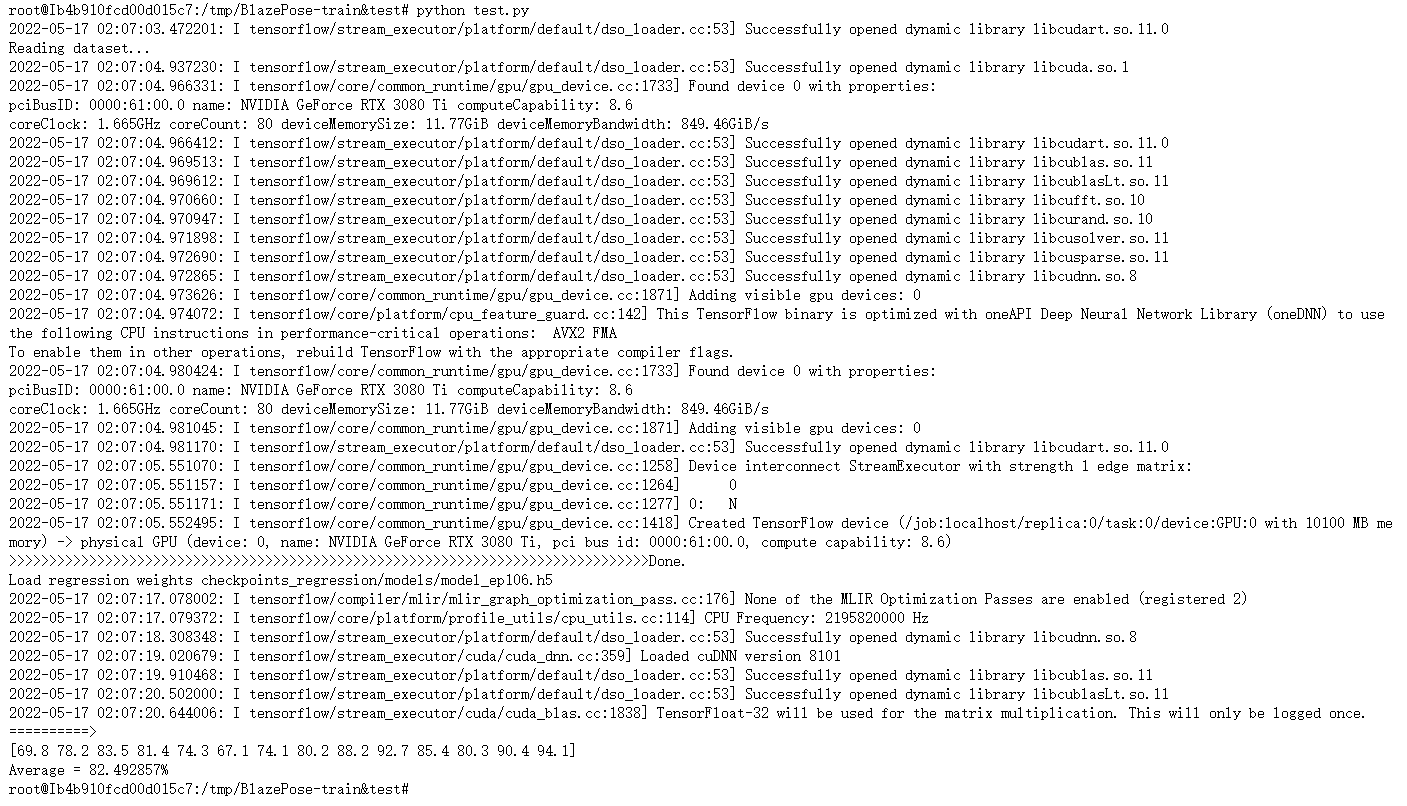
\includegraphics[width=1\linewidth]{acc_result}
\caption{模型在LSP数据集上的正确率}
\label{piture:17}
\end{figure}

\section{性能比较}
同时,本项目还与官方模型以及其它模型做了比较,其中,我们对模型在LSP数据集上做了PCK@0.2的结果对比,见表~\ref{acc}~和图~\ref{piture:27}~。此外,为了验证模型的轻量化,我们还在CPU型号是AMD Ryzen 7 5800H with RadeonGraphics 3.20 GHz上做了帧数对比,见表~\ref{fps}~和图~\ref{piture:28}~。


\begin{table}[htbp]
\caption{LSP数据集上一些模型的PCK}
\label{acc}
\vspace{0.5em}\centering\wuhao
\begin{tabular}{cc}
\toprule[1.5pt]
Model & LSP Dataset(PCK@0.2)  \\
\midrule[1pt]
官方模型(Heavy) & 97.5  \\
官方模型(Full) & 95.7  \\
官方模型(Lite)  & 93.5  \\
AlphaPose ResNet50 & 96.0  \\
Apple Vision  & 88.6  \\
Ours  & 82.5 \\
\bottomrule[1.5pt]
\end{tabular}
\end{table}

\begin{figure}
\centering
\begin{tikzpicture}[scale = 0.8]
	\begin{axis}[
	ybar, axis on top,
%	title={Cumulative Progress of Works},
	height=8cm, width=15.5cm,
	bar width=0.9cm,
	ymajorgrids, tick align=inside,
	major grid style={draw=white},
	enlarge y limits={value=.1,upper},
	ymin=0, ymax=100,
	axis x line*=bottom,
	axis y line*=right,
	y axis line style={opacity=0},
	tickwidth=0pt,
	enlarge x limits=true,
	legend style={
		at={(0.5,-0.2)},
		anchor=north,
		legend columns=-1,
		/tikz/every even column/.append style={column sep=0.5cm}
	},
	ylabel={PCK@0.2},
	symbolic x coords={
		LSP Dataset(PCK@0.2)},
	xtick=data,
	nodes near coords={
	\pgfmathprintnumber[precision=0]{\pgfplotspointmeta}
	}
    ]
	\addplot [draw=none, fill=blue!30] coordinates { (LSP Dataset(PCK@0.2),97.5) };
	\addplot [draw=none,fill=red!30] coordinates { (LSP Dataset(PCK@0.2),95.7) };
	\addplot [draw=none, fill=green!30] coordinates { (LSP Dataset(PCK@0.2),93.5) };
	\addplot [draw=none, fill=yellow!30] coordinates { (LSP Dataset(PCK@0.2),96.0) };
	\addplot [draw=none, fill=orange!30] coordinates { (LSP Dataset(PCK@0.2),88.6) };
	\addplot [draw=none, fill=purple!30] coordinates { (LSP Dataset(PCK@0.2),82.5) };

	\legend{BlazePose Heavy,BlazePose Full,BlazePose Lite,AlphaPose ResNet50,Apple Vision,Ours}
	\end{axis}
\end{tikzpicture}
\caption{模型在LSP数据集上PCK值的柱状图}
\label{piture:27}
\end{figure}


\begin{table}[htbp]
\caption{一些模型对于视频检测的帧数}
\label{fps}
\vspace{0.5em}\centering\wuhao
\begin{tabularx}{0.7\textwidth}{cX}
\toprule[1.5pt]
Model & FPS(AMD Ryzen 7 5800H with Radeon Graphics 3.20 GHz)  \\
\midrule[1pt]
官方模型(Heavy) & 38  \\
官方模型(Full) & 32  \\
官方模型(Lite) & 25  \\
OpenPose  & 6  \\
Ours  & 29 \\
\bottomrule[1.5pt]
\end{tabularx}
\end{table}

\begin{figure}
\centering
\begin{tikzpicture}[scale = 0.8]
\centering
	\begin{axis}[
	ybar, axis on top,
%	title={Cumulative Progress of Works},
	height=8cm, width=15.5cm,
	bar width=0.9cm,
	ymajorgrids, tick align=inside,
	major grid style={draw=white},
	enlarge y limits={value=.1,upper},
	ymin=0, ymax=40,
	axis x line*=bottom,
	axis y line*=right,
	y axis line style={opacity=0},
	tickwidth=0pt,
	enlarge x limits=true,
	legend style={
		at={(0.5,-0.2)},
		anchor=north,
		legend columns=-1,
		/tikz/every even column/.append style={column sep=0.5cm}
	},
	ylabel={帧数值},
	symbolic x coords={FPS(AMD Ryzen 7 5800H with RadeonGraphics 3.20 GHz)},
	xtick=data,
	nodes near coords={
	\pgfmathprintnumber[precision=0]{\pgfplotspointmeta}
	}
    ]
	\addplot [draw=none, fill=blue!30] coordinates {(FPS(AMD Ryzen 7 5800H with RadeonGraphics 3.20 GHz),38) };
	\addplot [draw=none,fill=red!30] coordinates {(FPS(AMD Ryzen 7 5800H with RadeonGraphics 3.20 GHz),32) };
	\addplot [draw=none, fill=green!30] coordinates {(FPS(AMD Ryzen 7 5800H with RadeonGraphics 3.20 GHz),25) };
	\addplot [draw=none, fill=orange!30] coordinates {(FPS(AMD Ryzen 7 5800H with RadeonGraphics 3.20 GHz),6) };
	\addplot [draw=none, fill=purple!30] coordinates {(FPS(AMD Ryzen 7 5800H with RadeonGraphics 3.20 GHz),29) };

	\legend{BlazePose Heavy,BlazePose Full,BlazePose Lite,OpenPose,Ours}
	\end{axis}
\end{tikzpicture}
\caption{模型在CPU上帧数的柱状图}
\label{piture:28}
\end{figure}


从表中数据我们可以看出,虽然我们根据官方Full版本复现的模型在准确度方面与原版有着差距,但是也已经达到了可以应用的程度,并且在轻量化方面也做到了媲美原版。

\section{API}
对于模型的部署,本项目没有设计函数,而是将我们的模型替换官方模型,再用MediaPipe库调用我们的模型,所以在部署模型之前,我们有必要介绍一下API。

\begin{enumerate}
\item STATIC\_IMAGE\_MODE

\qquad \quad 默认值是false,可以选择true。如果选择false,合适于检测视频,如图~\ref{piture:11}~所示,检测器只会在第一次出现人脸之前运行,当检测到人脸之后,检测器定位图像的姿态ROI,然后传给跟踪器,预测出33个关键点的坐标。对于检测到人脸之后,会从前一帧的33个关键点中预测出ROI,而不会再次启用检测器;对于true,就是每一帧都会启用检测器,这会大大加大CPU的负担。

\item MODEL\_COMPLEXITY

\qquad \quad 可选值是$0,1,2$分别对于着官方模型的Lite、Full和Heavy版本。由于我们复现的是官方的Full模型,所以在此我们只能选择$1$,值得说明的是,该参数的默认值就是$1$。

\item UPPER\_BODY\_ONLY

\qquad \quad 设置为true表示识别出全身33个关键点;设置为false表示识别出上半身的25个关键点。

\item SMOOTH\_LANDMARKS

\qquad \quad 设置为true,将会平滑关键点,从而减少抖动。但如果检测单张图像,即STATIC\_IMAGE\_MODE也设置为true,则忽略该参数。

\item MIN\_DETECTION\_CONFIDENCE

\qquad \quad 置信度阈值,范围是$[0.0,1.0]$,默认设置为0.5。在人体检测器中,如果该像素点的置信度超过了设定的阈值,则认为该像素点为人体。

\item MIN\_TRACKING\_CONFIDENCE

\qquad \quad 追踪阈值,范围是$[0.0,1.0]$,默认设置为0.5。在追踪器中,如果超过该阈值,则表示成功检测到33个关键点,否则将会在下一帧中调用人体检测器。但如果STATIC\_IMAGE\_MODE也设置为true,即检测单张图像,则忽略该参数。
\end{enumerate}

\section{基于BlazePose的姿态识别}

\subsection{电脑端的姿态识别}
这里对于在电脑端部署模型,本项目并没有另外设计函数,本项目采取的方法是将训练好的.h5模型用tensorflow工具转换成.tflite模型,再将其替换谷歌官方的MediaPipe库中的模型,从而可以直接调用谷歌MediaPipe库的方法来测试我们的模型。

\subsubsection{检测人物并蒙版抠图}
该部分主要将图像中的人物检测出来并蒙版抠图,主要是为后续的关键点检测提供ROI。

值得注意的一点是,我们需要使用opencv库提供的cvtColor颜色空间转换函数,将读入的BGR格式转换成matplotlib可输出的RGB格式。

实现方法主要是使用了Selfie Segmentation工具包,该工具包会给出每个像素点是人体一部分的概率,我们设定一个阈值(0.5),如果概率小于阈值,我们不输出该像素点;如果概率大于该阈值,我们则认为该像素点是人体的一部分,输出该像素点。

效果如图~\ref{picture:17}~所示。

\begin{figure}
\centering
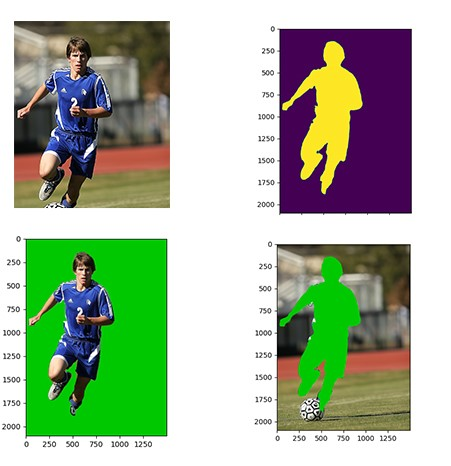
\includegraphics[width=0.7\linewidth]{mask}
\caption{左上为原图,后上是蒙版\\左下是前景人像,右下为抠掉前景人像的背景}
\label{picture:17}
\end{figure}

\subsubsection{单张图片检测}
本部分完成的是对于单张图片的BlazePose关键点检测。函数主要调用了MediaPipe库。

同时由于单张图片的检测会使得模型第一次检测到人体,因此一定会调用人检测器定位ROI。

我们会获得33个关键点的各自像素坐标,然后将该关键点染色并连接

对于各个关键点用不同的颜色加以区分。

主要代码如下:
\begin{python}
for i in range(33):
  h, w = img.shape[0], img.shape[1]
  
  cx = int(results.pose_landmarks.landmark[i].x * w)
  cy = int(results.pose_landmarks.landmark[i].y * h)
  cz = results.pose_landmarks.landmark[i].z

  radius = 10

  if i == 0: # 鼻
    img = cv2.circle(img,(cx,cy), radius, (0,0,255), -1)
  elif i in [11,12]: # 肩
    img = cv2.circle(img,(cx,cy), radius, (223,155,6), -1)
  elif i in [23,24]: # 髋
    img = cv2.circle(img,(cx,cy), radius, (1,240,255), -1)
  elif i in [13,14]: # 肘
    img = cv2.circle(img,(cx,cy), radius, (140,47,240), -1)
  elif i in [25,26]: # 膝
    img = cv2.circle(img,(cx,cy), radius, (0,0,255), -1)
  elif i in [15,16,27,28]: # 手腕、脚腕
    img = cv2.circle(img,(cx,cy), radius, (223,155,60), -1)
  elif i in [17,19,21]: # 左手
    img = cv2.circle(img,(cx,cy), radius, (94,218,121), -1)
  elif i in [18,20,22]: # 右手
    img = cv2.circle(img,(cx,cy), radius, (16,144,247), -1)
  elif i in [27,29,31]: # 左脚
    img = cv2.circle(img,(cx,cy), radius, (29,123,243), -1)
  elif i in [28,30,32]: # 右脚
    img = cv2.circle(img,(cx,cy), radius, (193,182,255), -1)
  elif i in [9,10]: # 嘴
    img = cv2.circle(img,(cx,cy), radius, (205,235,255), -1)
  elif i in [1,2,3,4,5,6,7,8]: # 眼、脸颊
    img = cv2.circle(img,(cx,cy), radius, (94,218,121), -1)
  else: # 其它关键点
    img = cv2.circle(img,(cx,cy), radius, (0,255,0), -1)

look_img(img)
\end{python}

结果如图~\ref{picture:18}~所示。

\begin{figure}
\centering
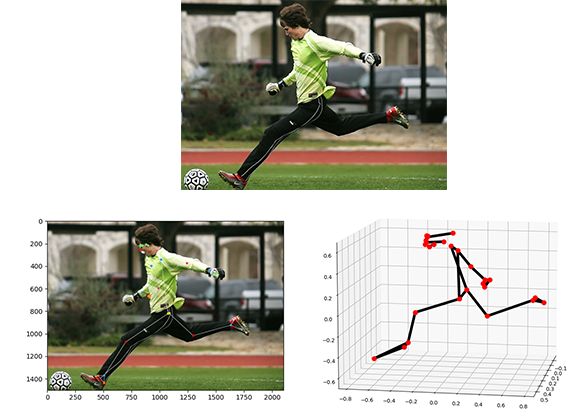
\includegraphics[width=0.7\linewidth]{Single}
\caption{上方为原图,左下为关键点骨架图,右下为三维图}
\label{picture:18}
\end{figure}

\subsubsection{在线摄像头检测}

本部分主要是使用BlazePose模型对摄像头实时检测。

主要代码和单张图片类似,不过输入换成了摄像头。

另外值得说明的是,对于连续视频流,我们只会在第一个人体出来的帧之前帧调用人检测器,此后的帧只会在上一帧的33个关键点中预测出当前帧的ROI。从而使得模型更加轻量化,更加实时化。

结果如图~\ref{picture:19}~所示。

\begin{figure}
\centering
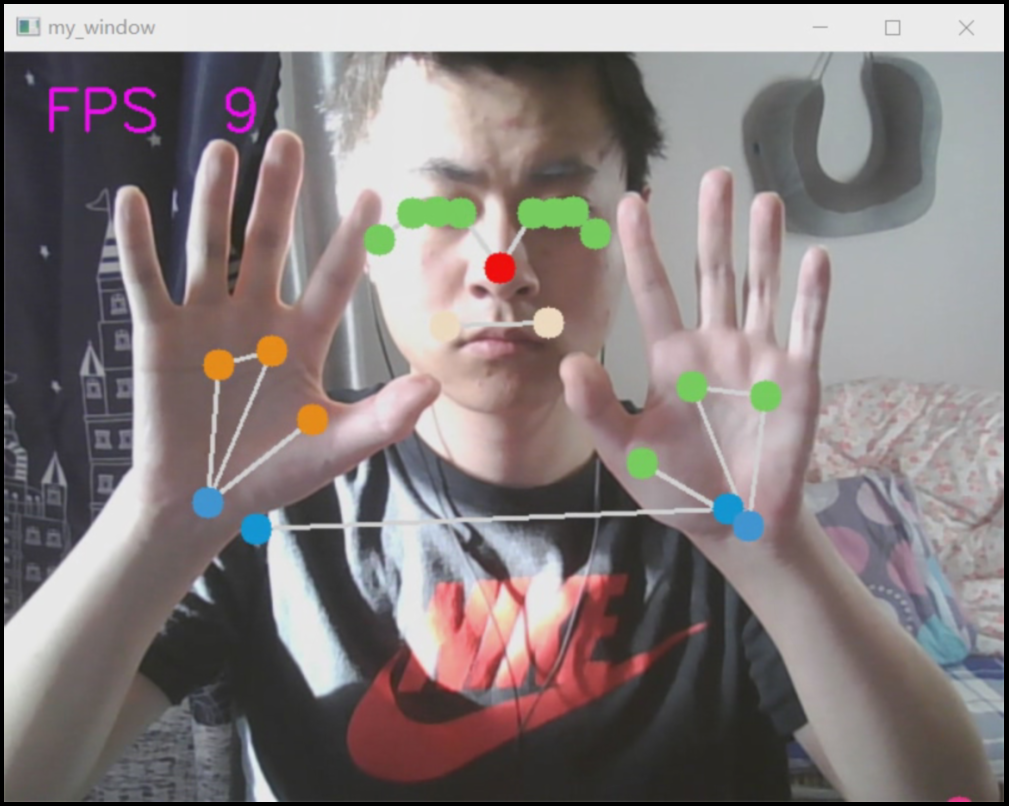
\includegraphics[width=0.7\linewidth]{camera}
\caption{摄像头实时检测截图}
\label{picture:19}
\end{figure}

\subsubsection{离线视频检测}

本部分主要是使用BlazePose模型对离线视频检测。

本部分核心代码和实时检测摄像头相同,主要加了一个生成视频的函数。这样使得输入输出均为视频。

结果如图~\ref{picture:20}~所示。

\begin{figure}[!h]
\setlength{\subfigcapskip}{-1bp}
\centering
\begin{minipage}{\textwidth}
\centering
\subfigure[原视频截图]{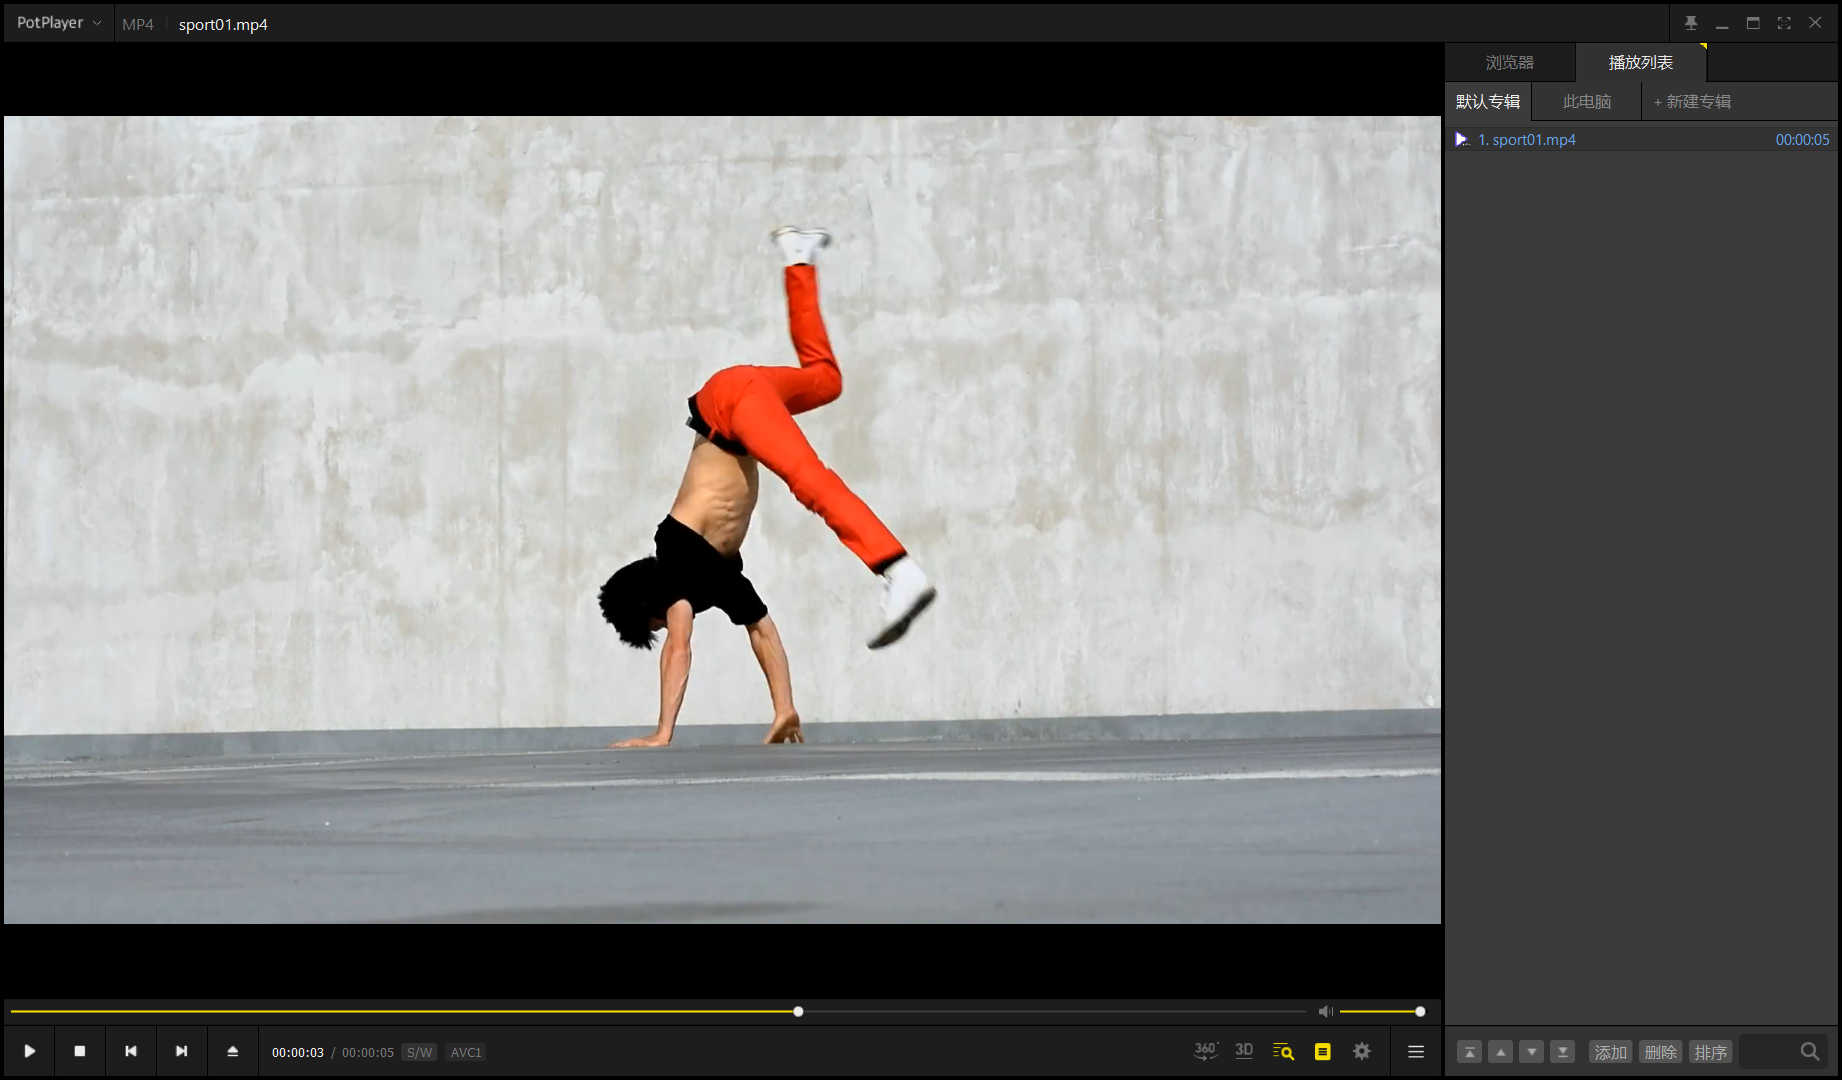
\includegraphics[width=0.45\textwidth]{video1}}
\hspace{2em}
\subfigure[输出视频截图]{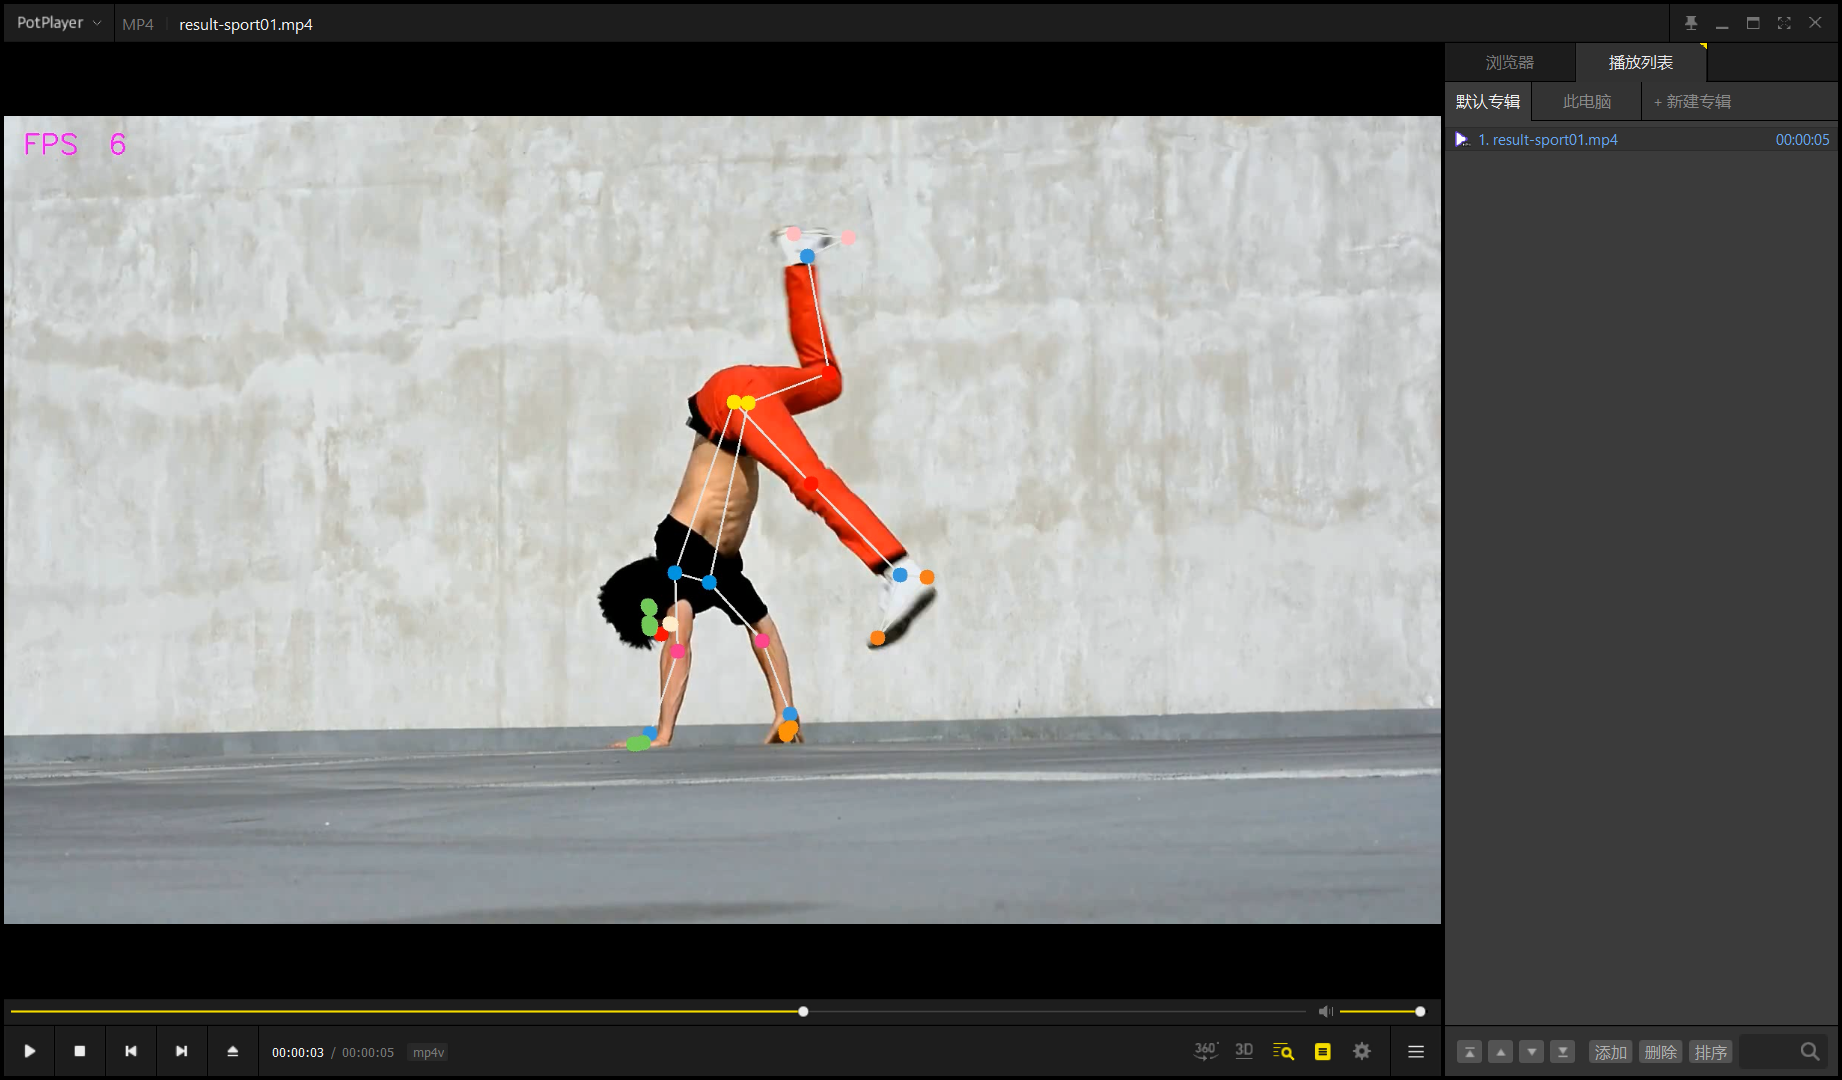
\includegraphics[width=0.45\textwidth]{video2}}
\end{minipage}
\vspace{0.2em}
\caption{离线视频检测}
\label{picture:20}
\end{figure}


\subsection{移动端的姿态识别}

对于移动端的部署,本项目采用腾讯的TNN\footnote{\href{https://github.com/Tencent/TNN}{https://github.com/Tencent/TNN}}轻量化框架,其提供了各种框架模型 (如 TensorFlow、PyTorch、Caffe等) 转化为TNN模型文件的脚本,还有丰富的demo可供学习。其架构图如图~\ref{picture:22}~所示。

\begin{figure}
\centering
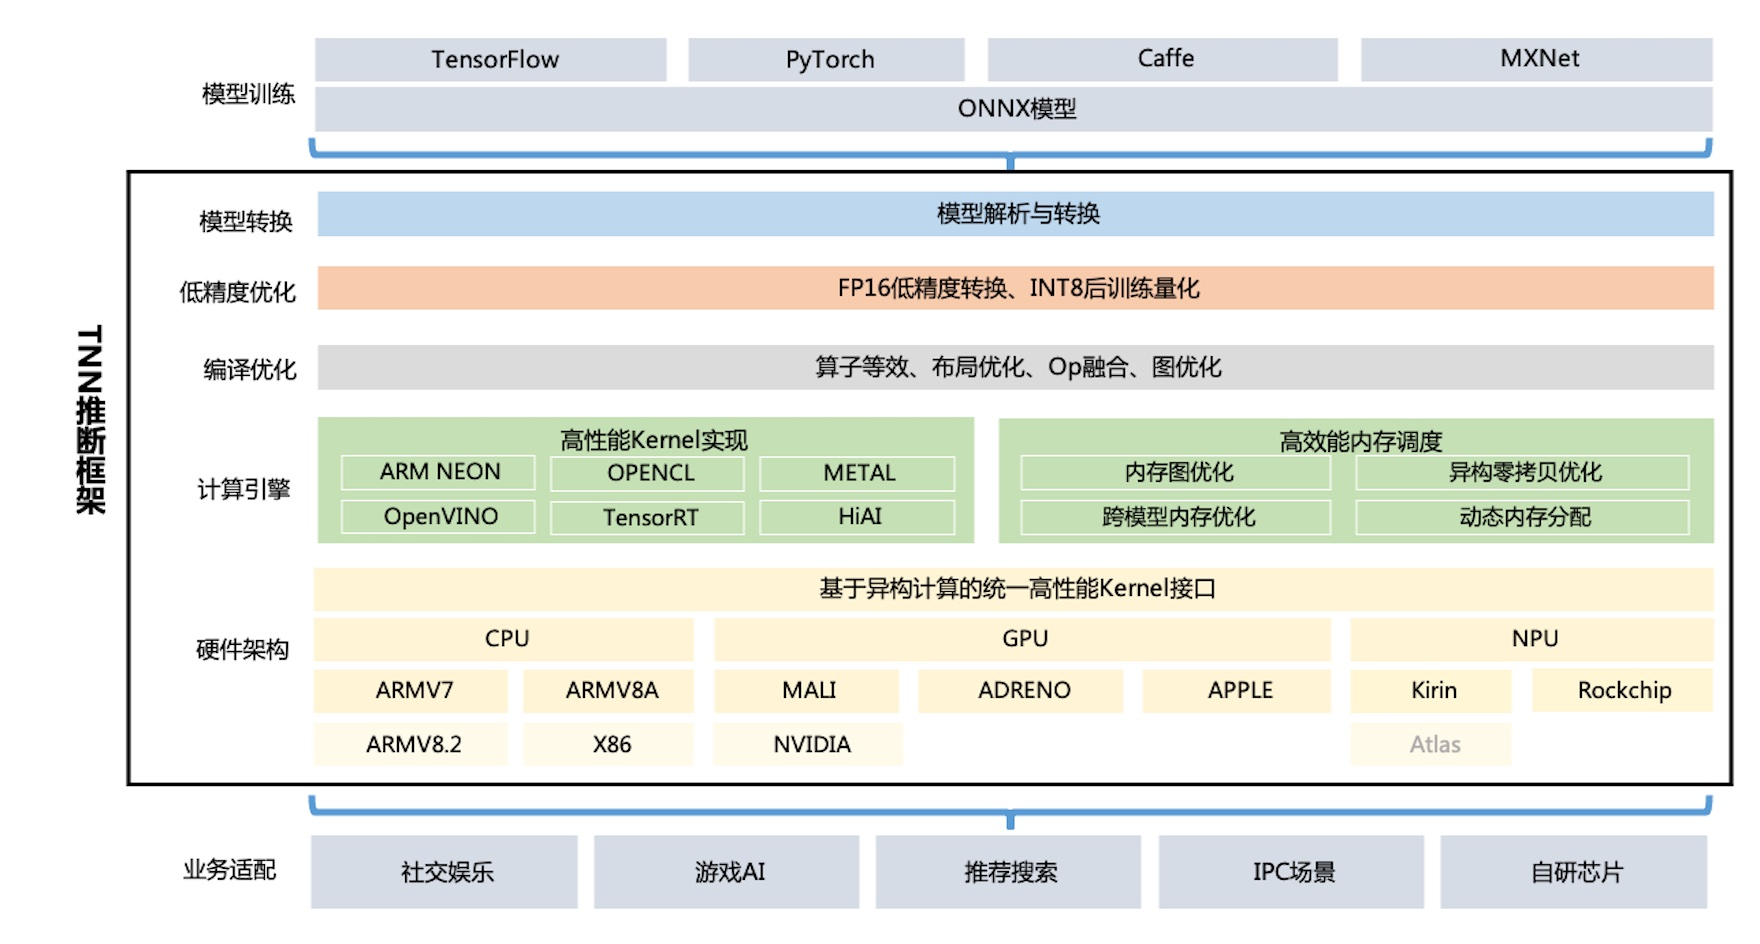
\includegraphics[width=0.7\linewidth]{architecture}
\caption{TNN架构图}
\label{picture:22}
\end{figure}

首先我们使用TNN官方的转换脚本\footnote{\href{https://github.com/Tencent/TNN/blob/master/doc/cn/user/convert.md}{https://github.com/Tencent/TNN/blob/master/doc/cn/user/convert.md}}将我们的.tflite模型转换成.tnn模型

然后编译TNN引擎,我们选择了arm和OpenCL这两个平台。对于这两个平台,TNN都有极其方便的脚本\footnote{\href{https://github.com/Tencent/TNN/blob/master/doc/cn/user/compile.md}{https://github.com/Tencent/TNN/blob/master/doc/cn/user/compile.md}}。

最后,我们构建了一个调用编译好的TNN引擎进行推理的应用程序,从而在手机端部署了我们的模型。

移动端app对于摄像头实时检测的结果截图如图~\ref{picture:23}~所示。

\begin{figure}[!h]
\setlength{\subfigcapskip}{-1bp}
\centering
\begin{minipage}{\textwidth}
\centering
\subfigure[主界面截图]{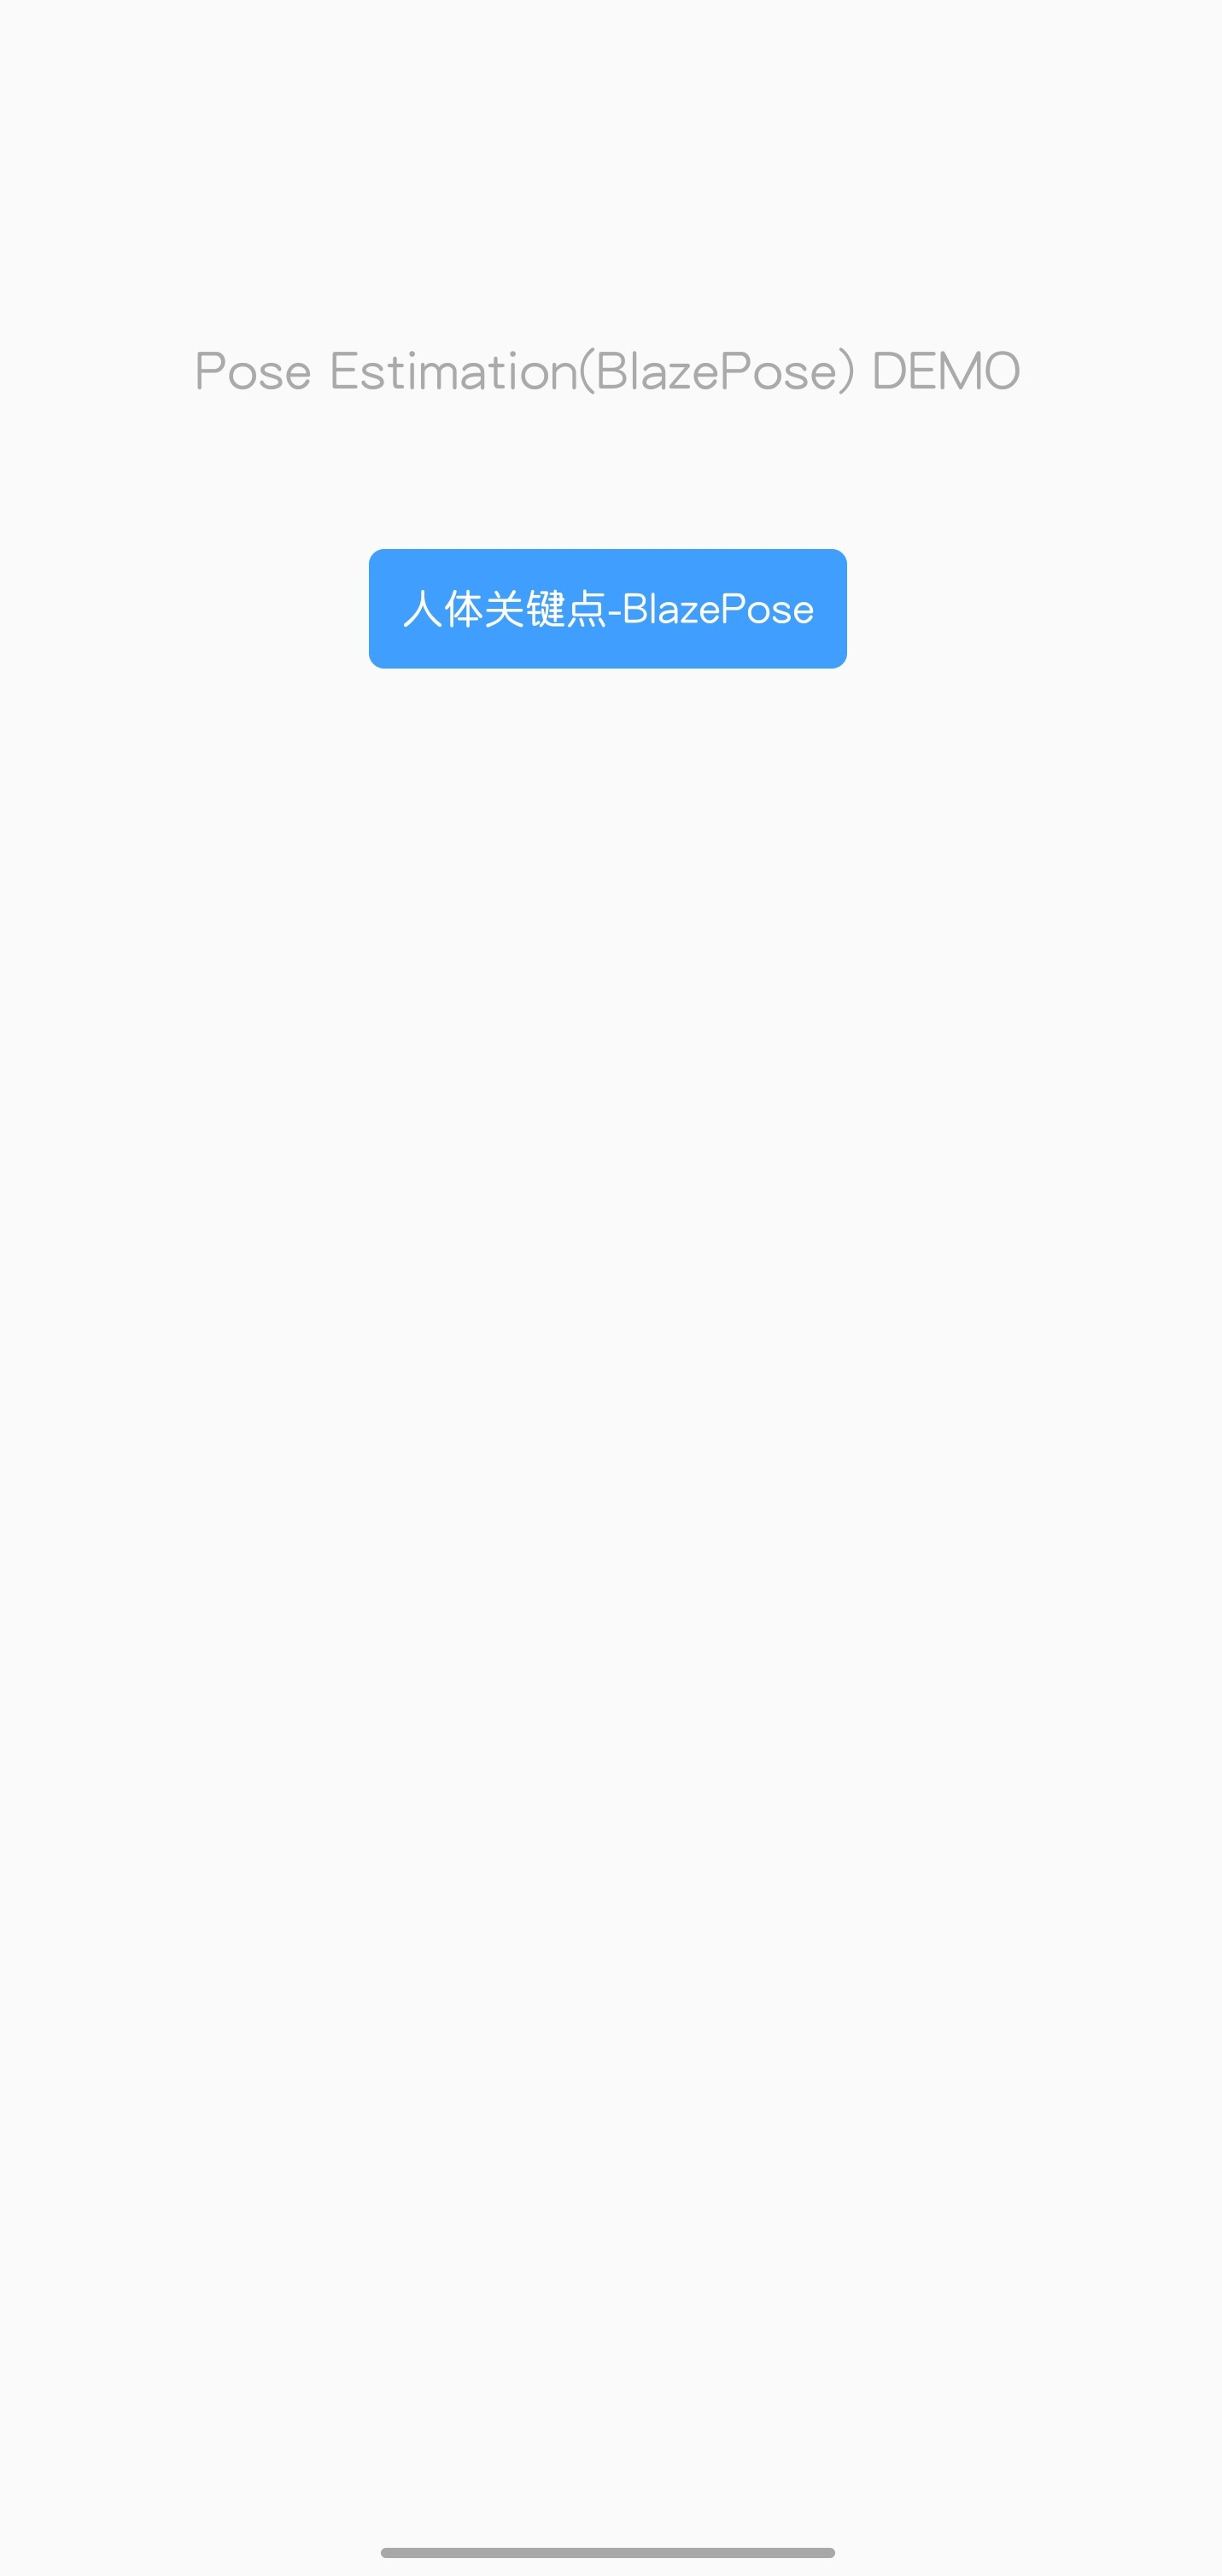
\includegraphics[width=0.18\textwidth]{mobile1}}
\hspace{2em}
\subfigure[arm上半身截图]{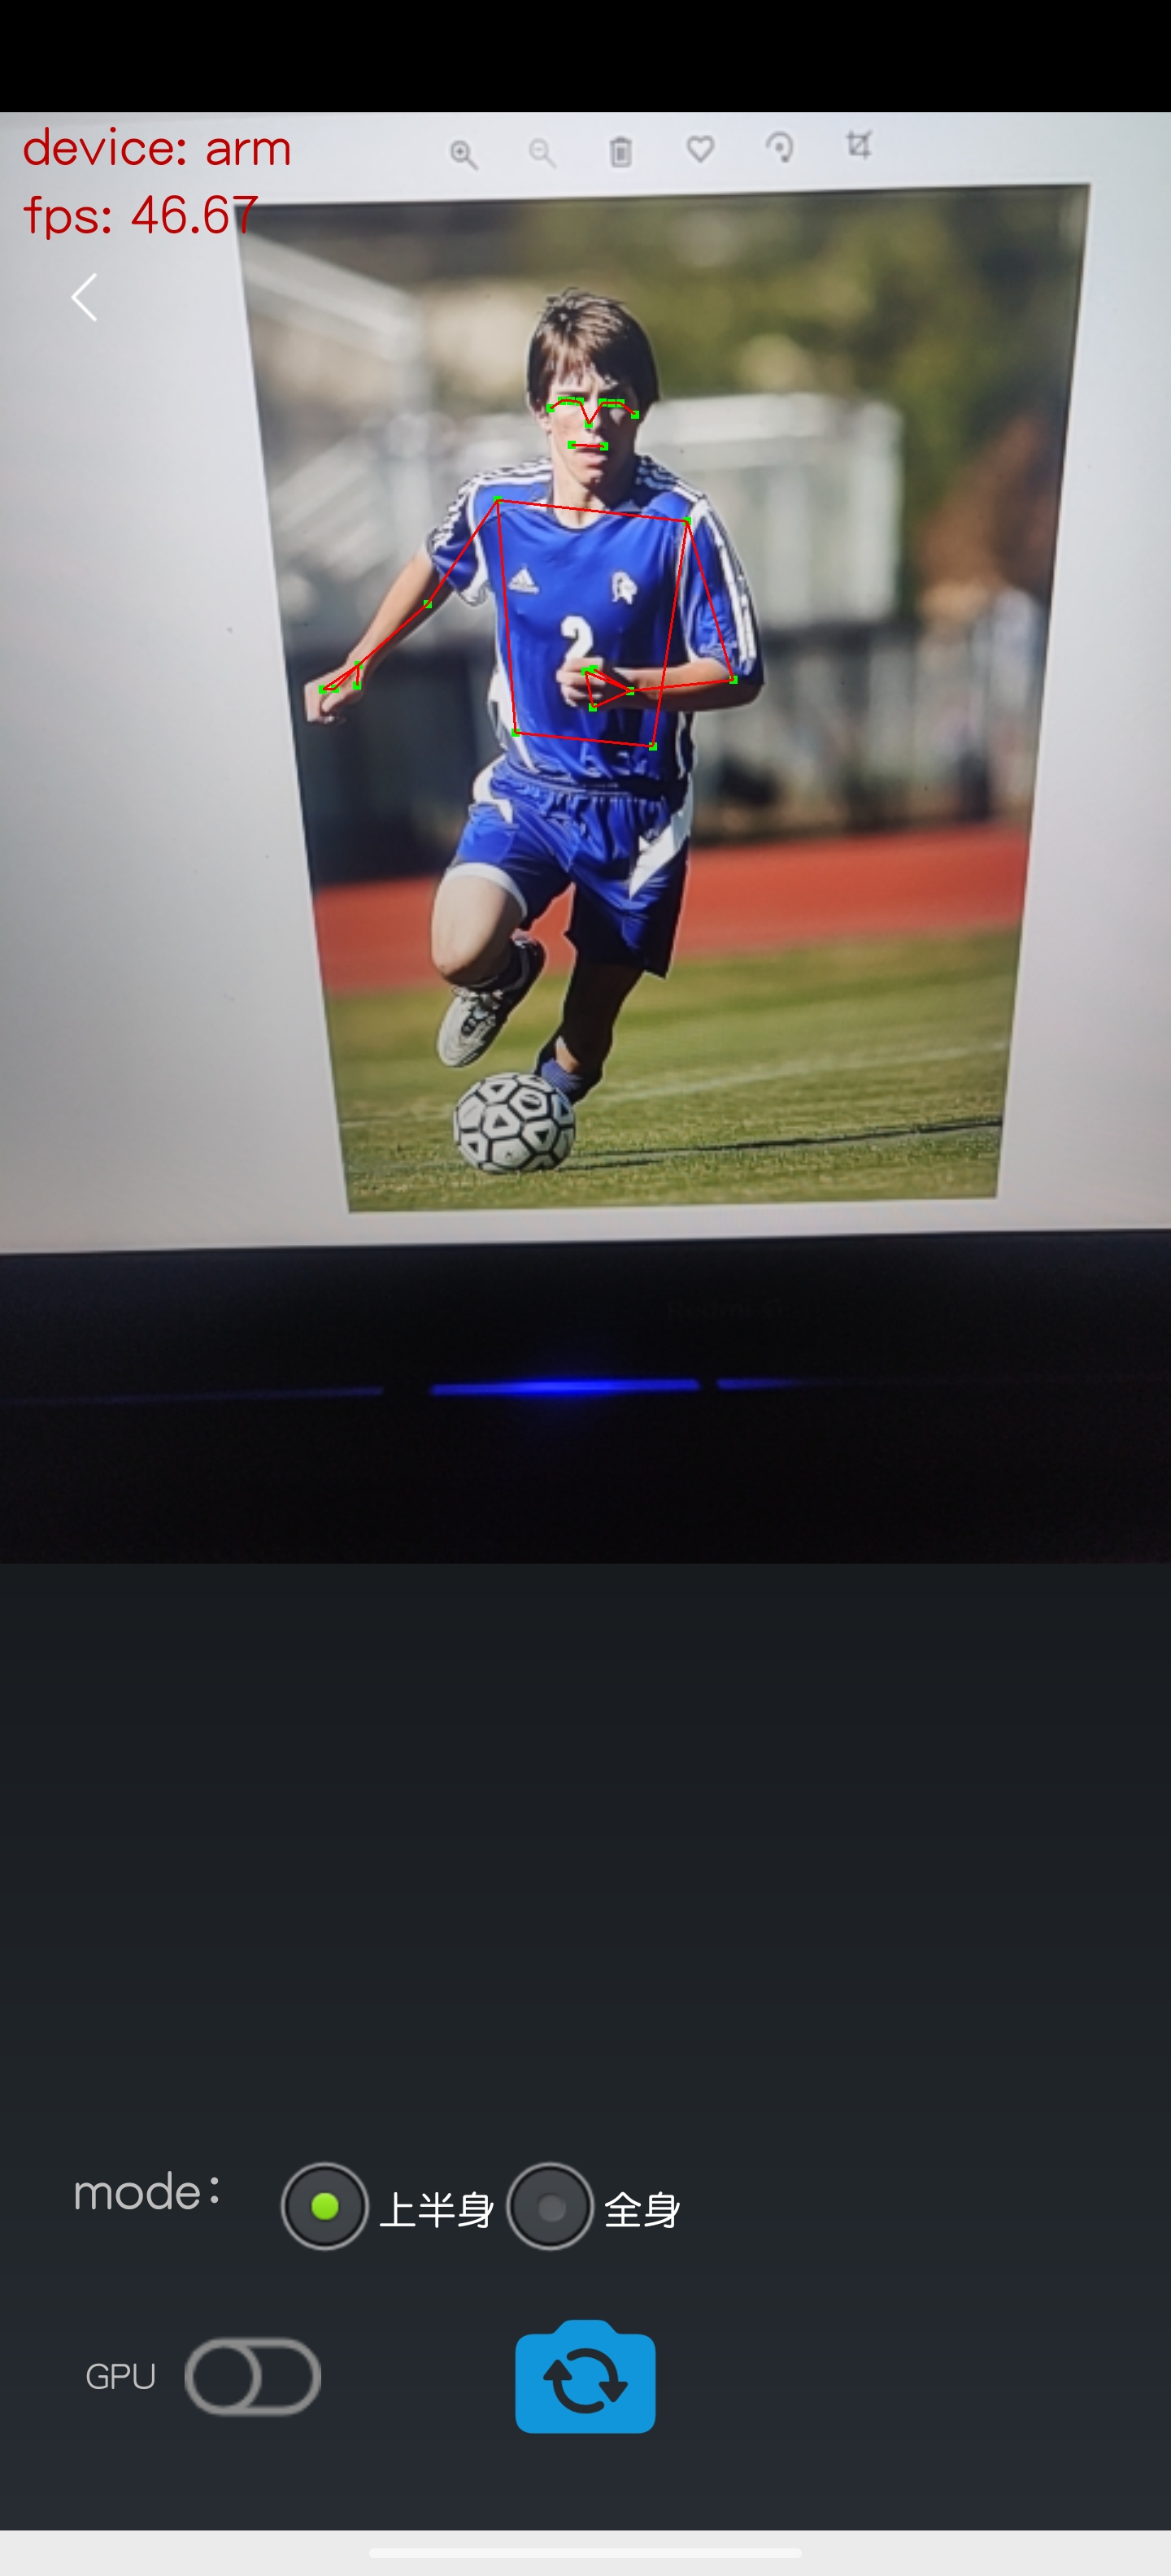
\includegraphics[width=0.18\textwidth]{mobile2}}
\hspace{2em}
\subfigure[arm全身截图]{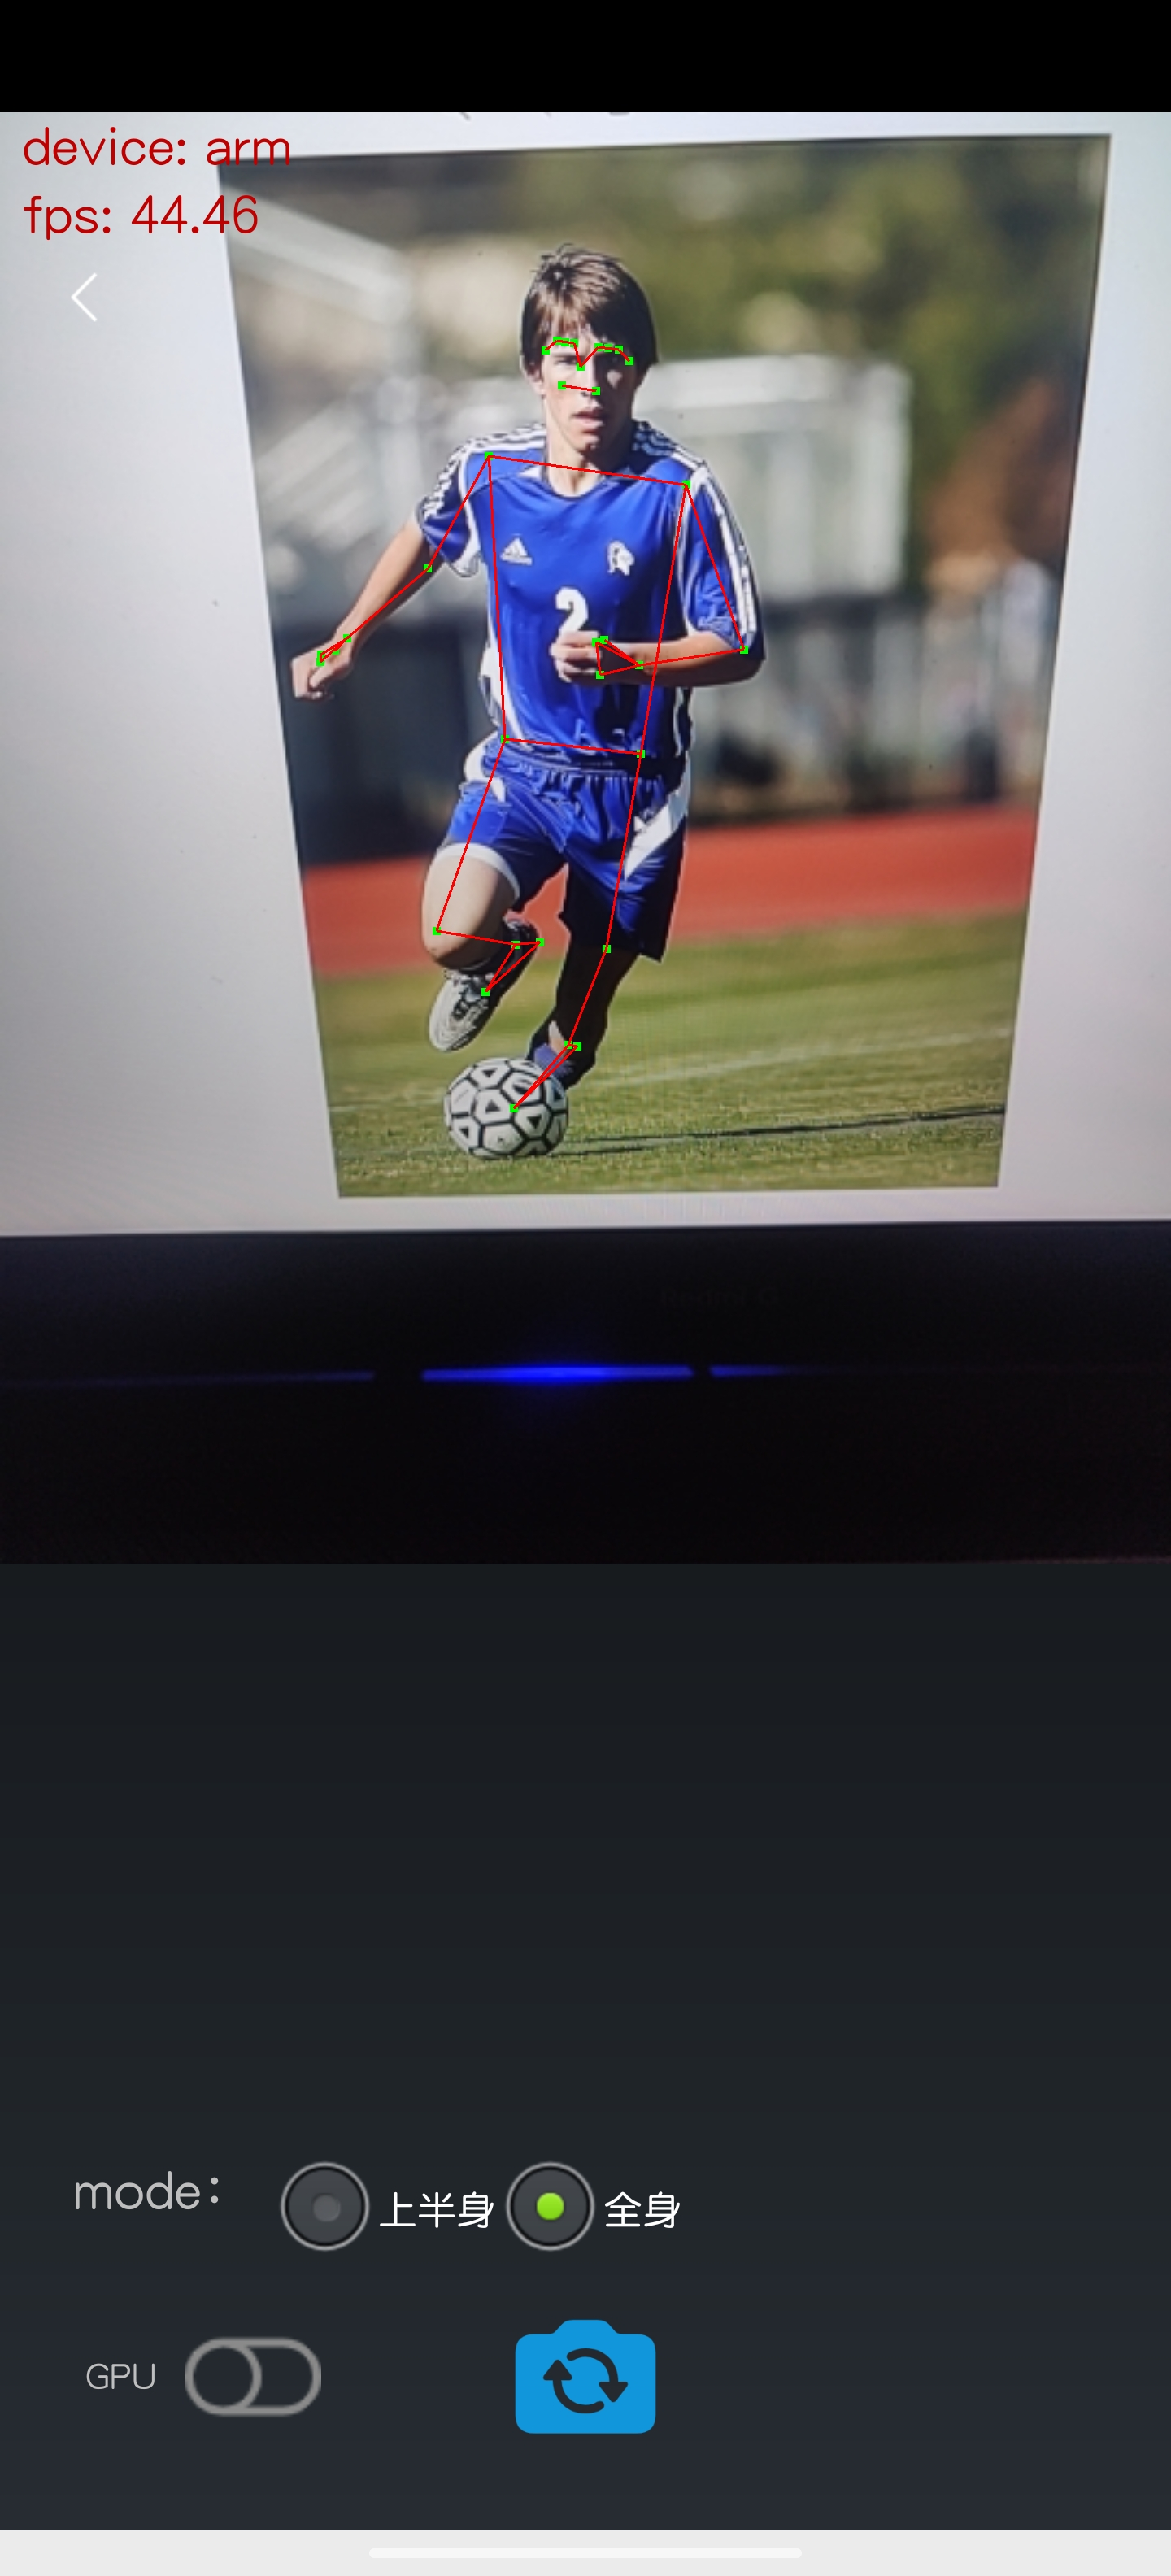
\includegraphics[width=0.18\textwidth]{mobile3}}
\end{minipage}
\centering
\begin{minipage}{\textwidth}
\centering
\subfigure[OpenCL上半身截图]{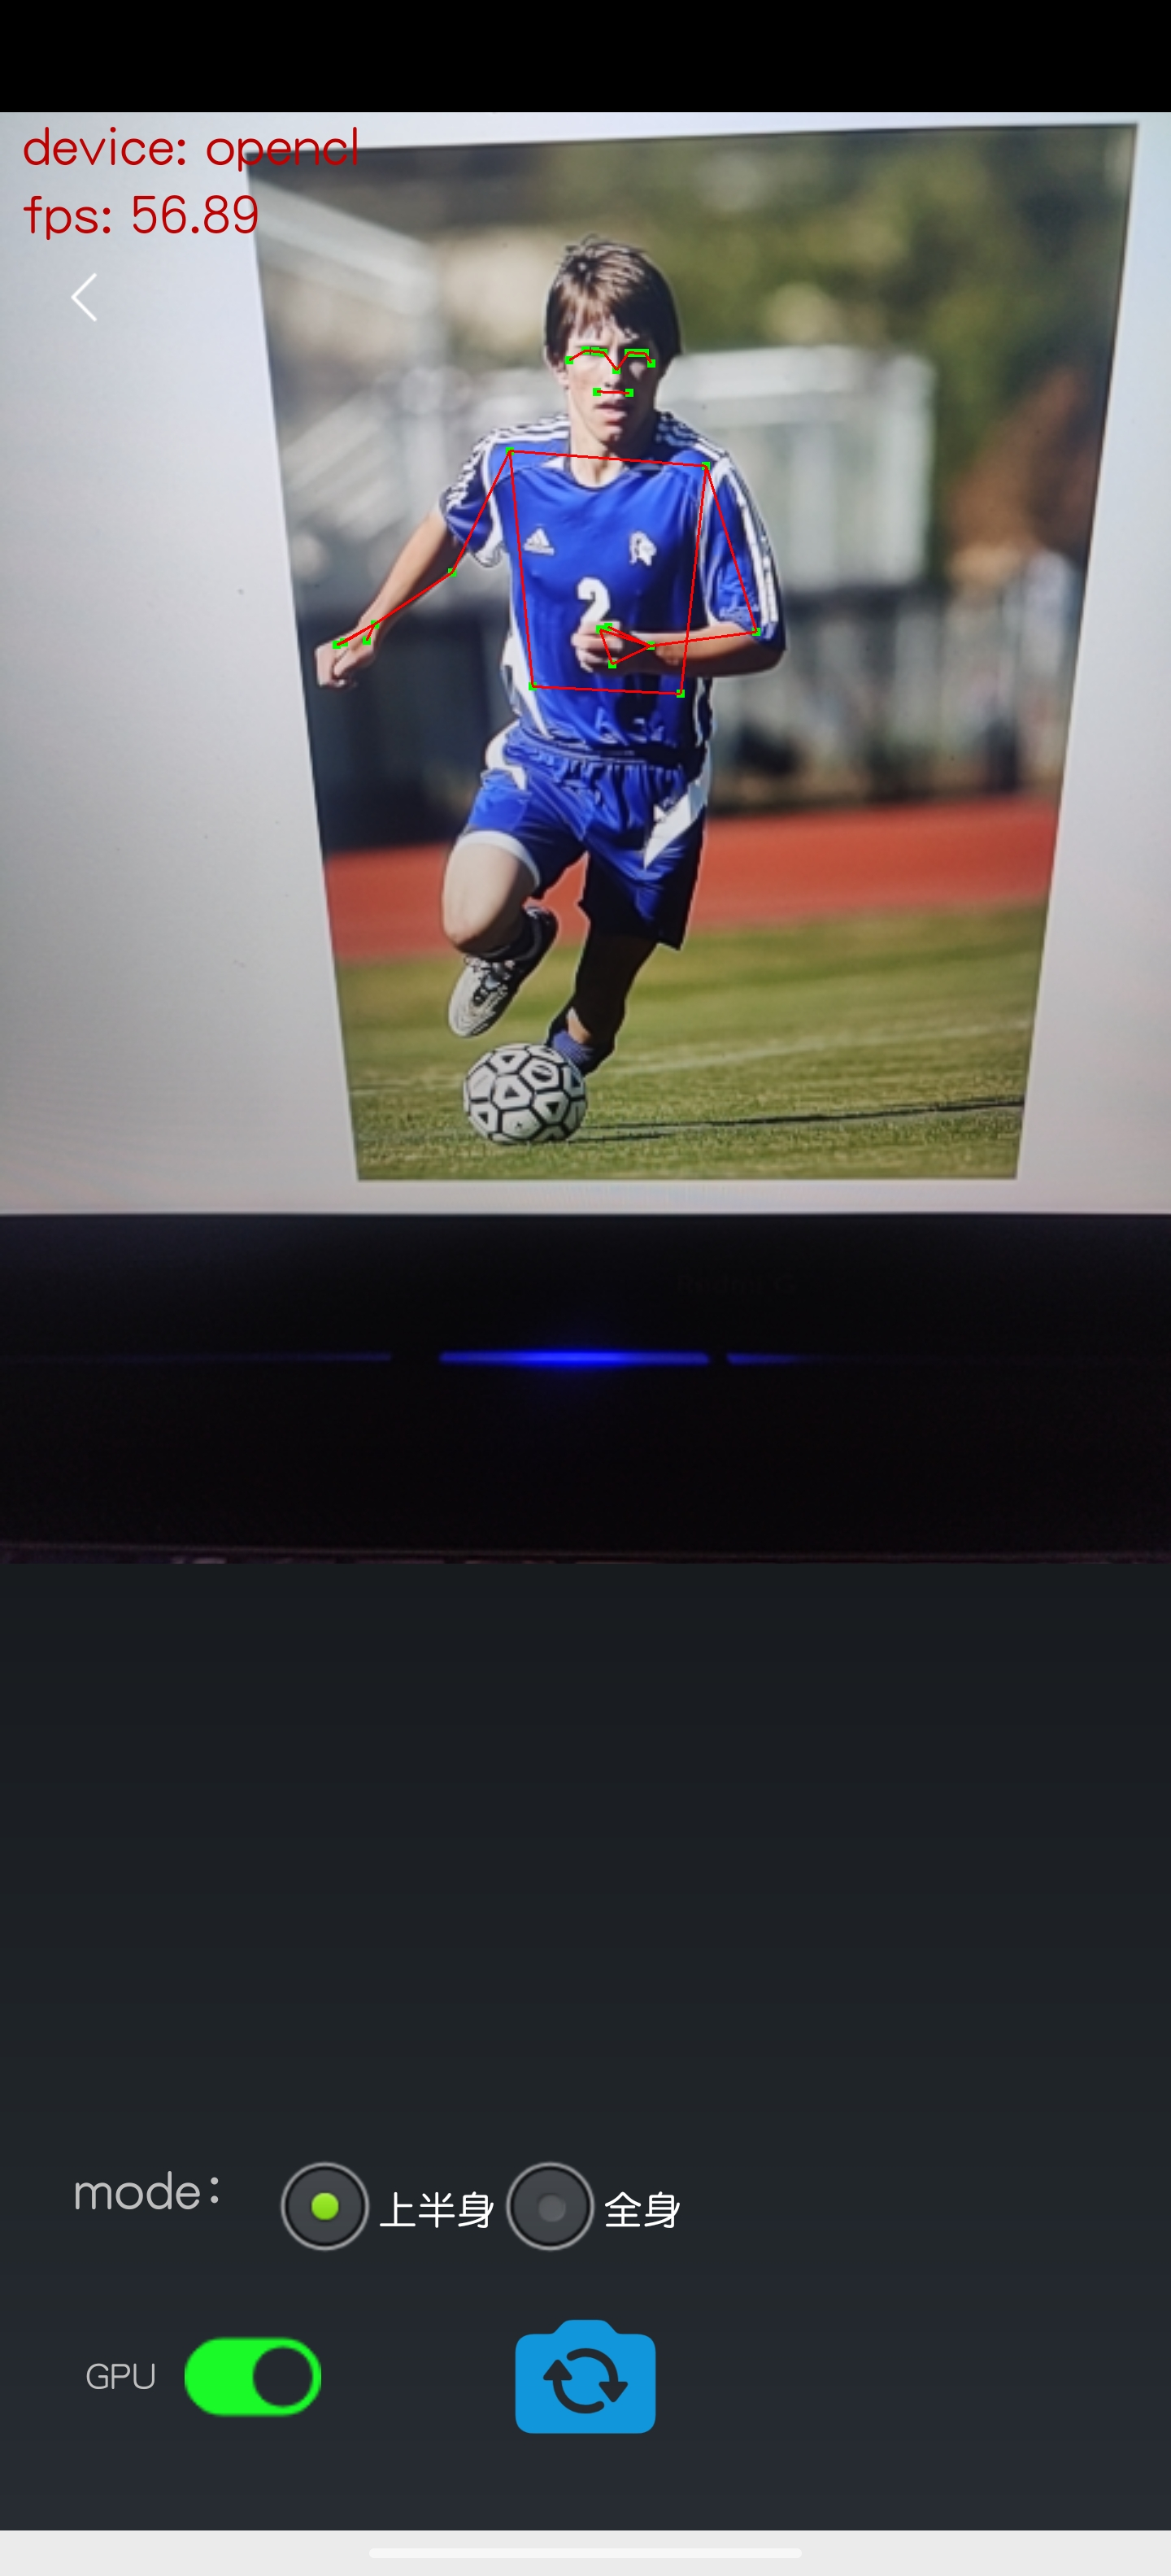
\includegraphics[width=0.18\textwidth]{mobile4}}
\hspace{2em}
\subfigure[OpenCL全身截图]{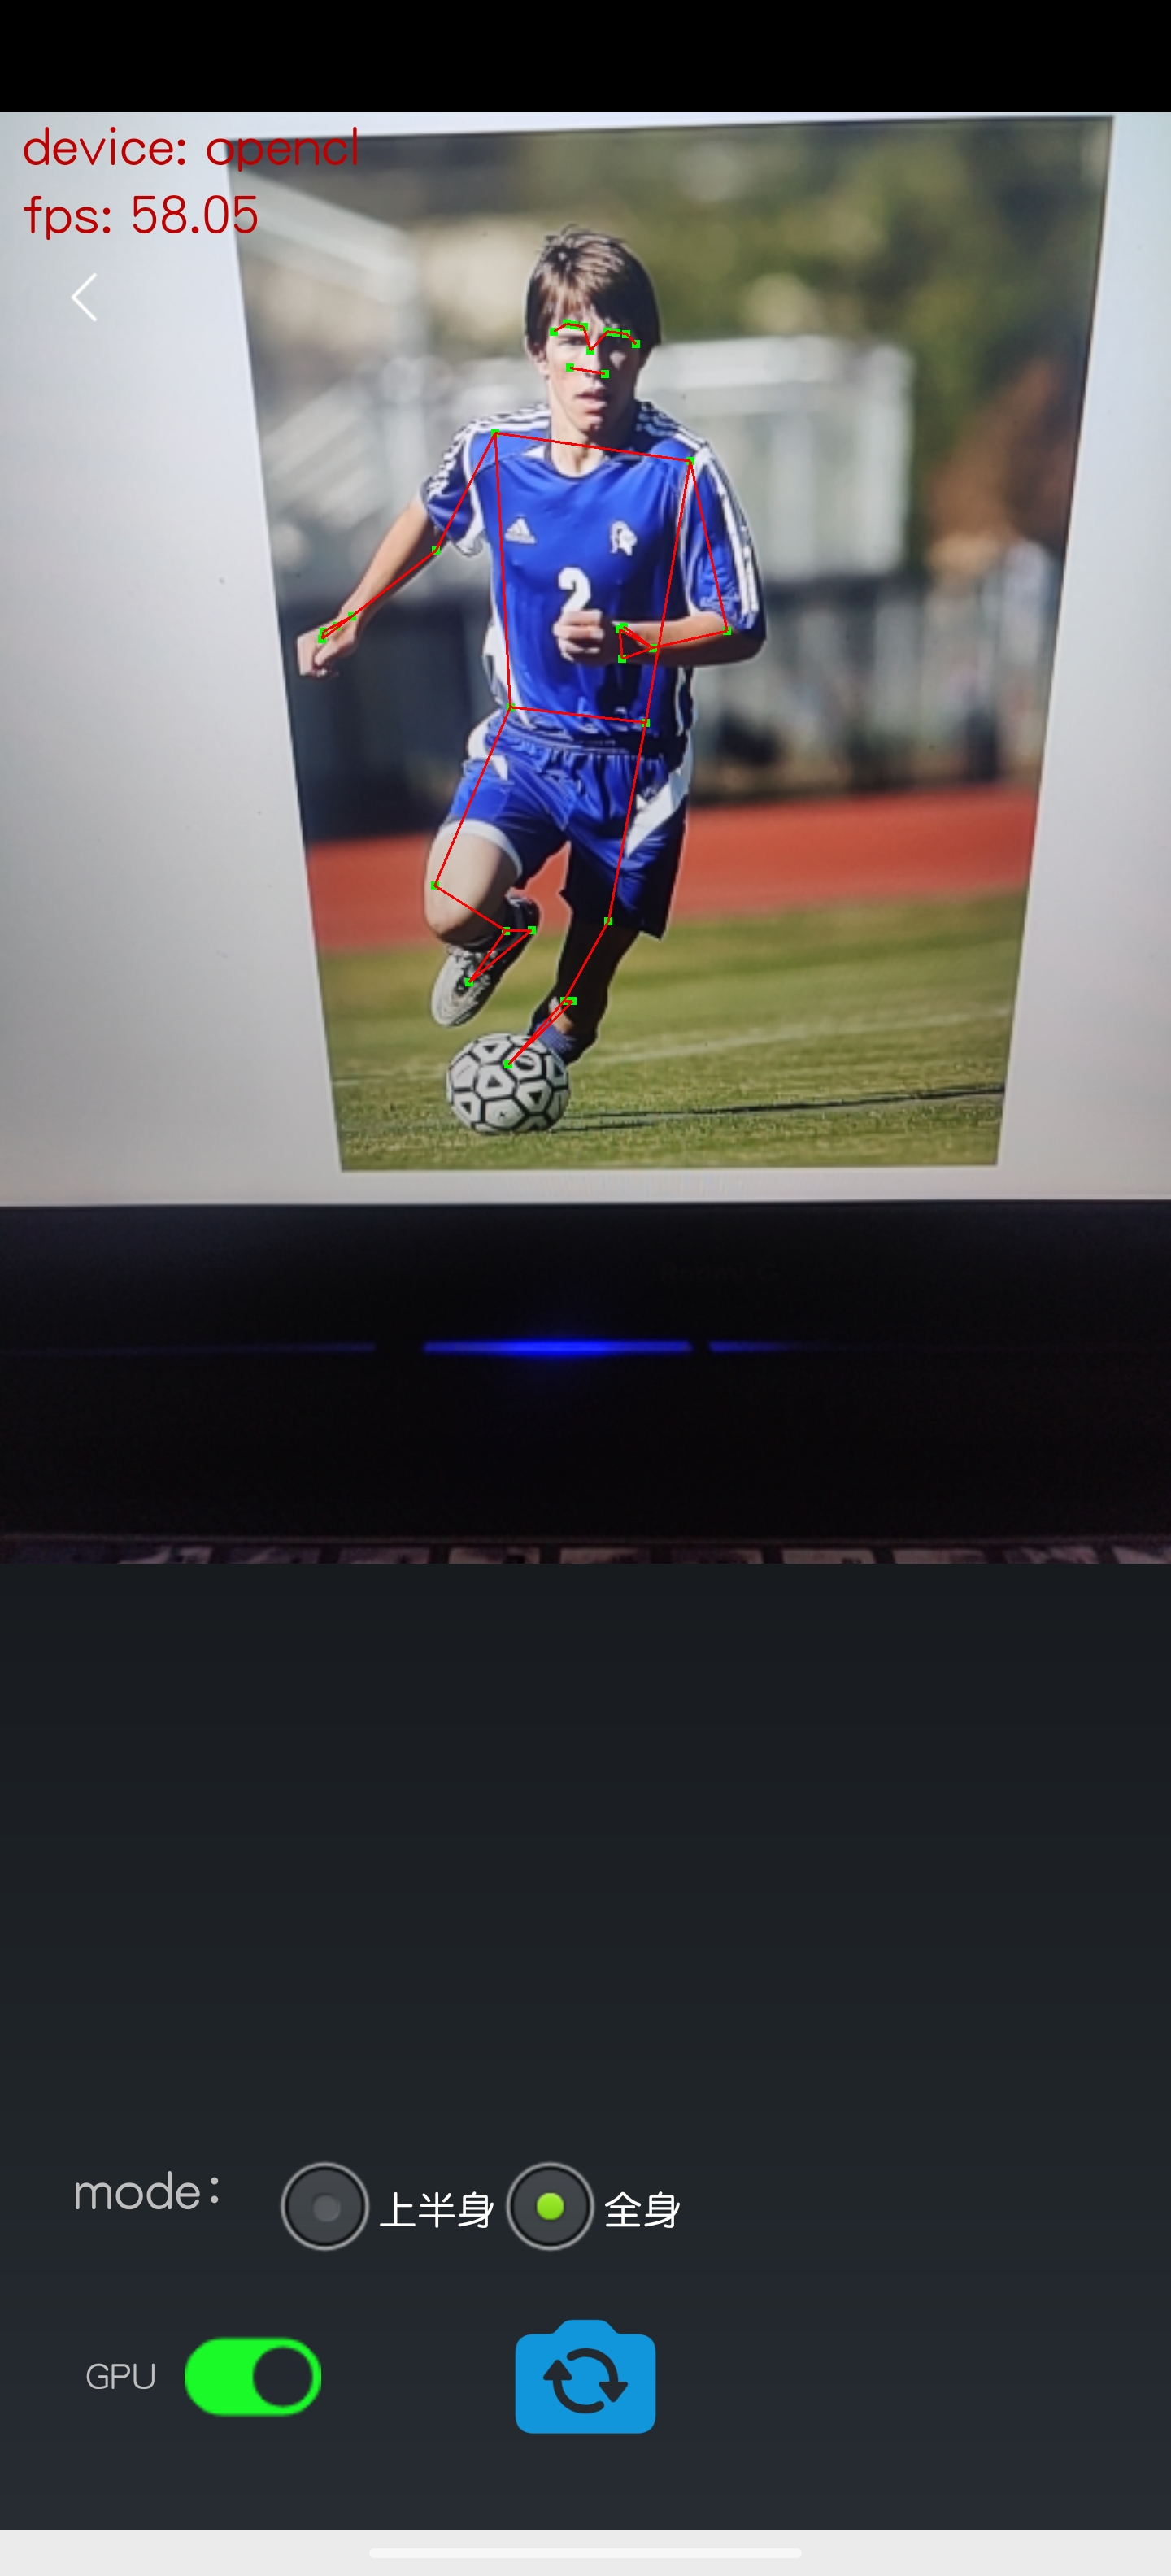
\includegraphics[width=0.18\textwidth]{mobile5}}
\end{minipage}
\vspace{0.2em}
\caption{移动端app截图}
\label{picture:23}
\end{figure}

\section{基于BlazePose的姿态模仿}

\subsection{虚拟机器人的姿态模仿}

本部分使用了unity3d创建了一个拥有33个关键点的虚拟火柴人。

再用python实时检测摄像头或者视频输入。获得每个点的相对位置和角度角度。使用UDP,创建了在本机``127.0.0.1''上的5052端口,在此端口上进行数据传输,将每个点的位置传输到unity中,从而使得机器人能够姿态模仿。

对于unity3d的虚拟火柴人进行姿态模仿结果如图~\ref{picture:24}~所示。

\begin{figure}[!h]
\setlength{\subfigcapskip}{-1bp}
\centering
\begin{minipage}{\textwidth}
\centering
\subfigure{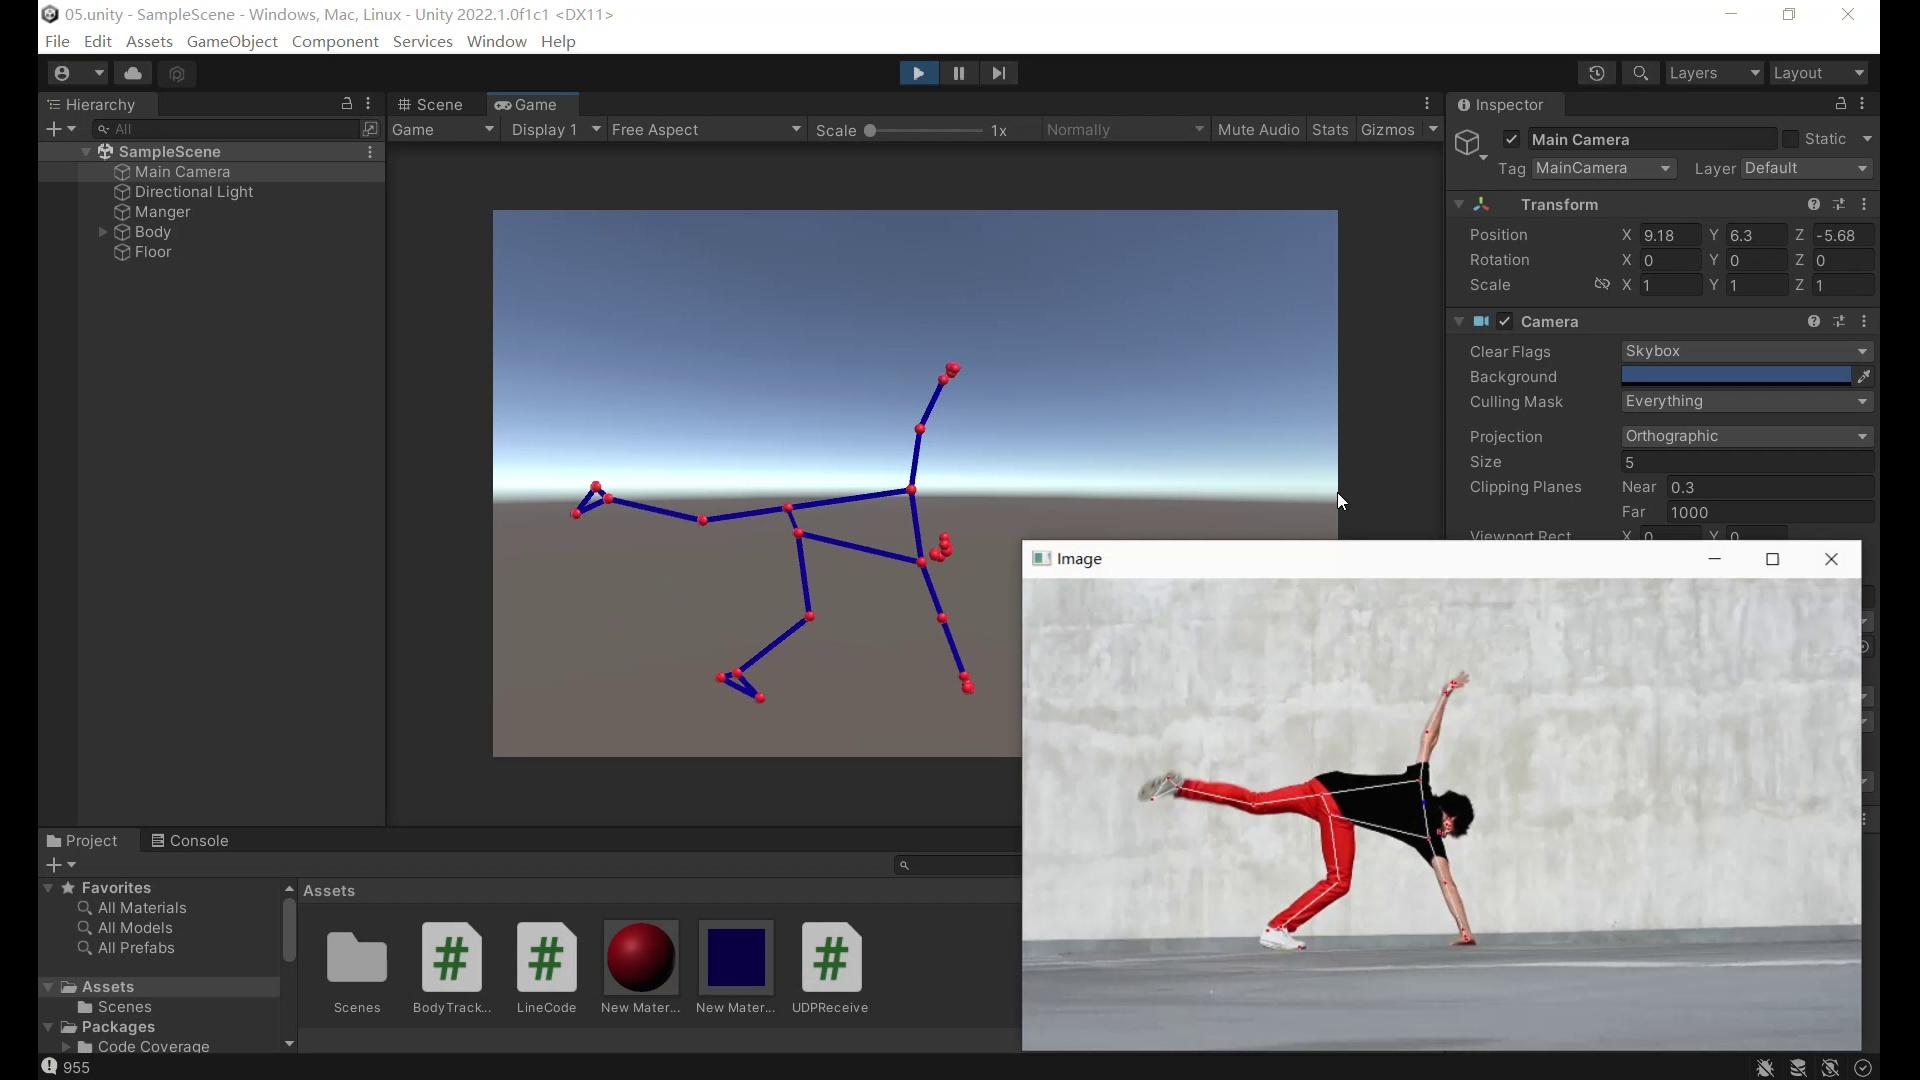
\includegraphics[width=0.24\textwidth]{unity1}}
\subfigure{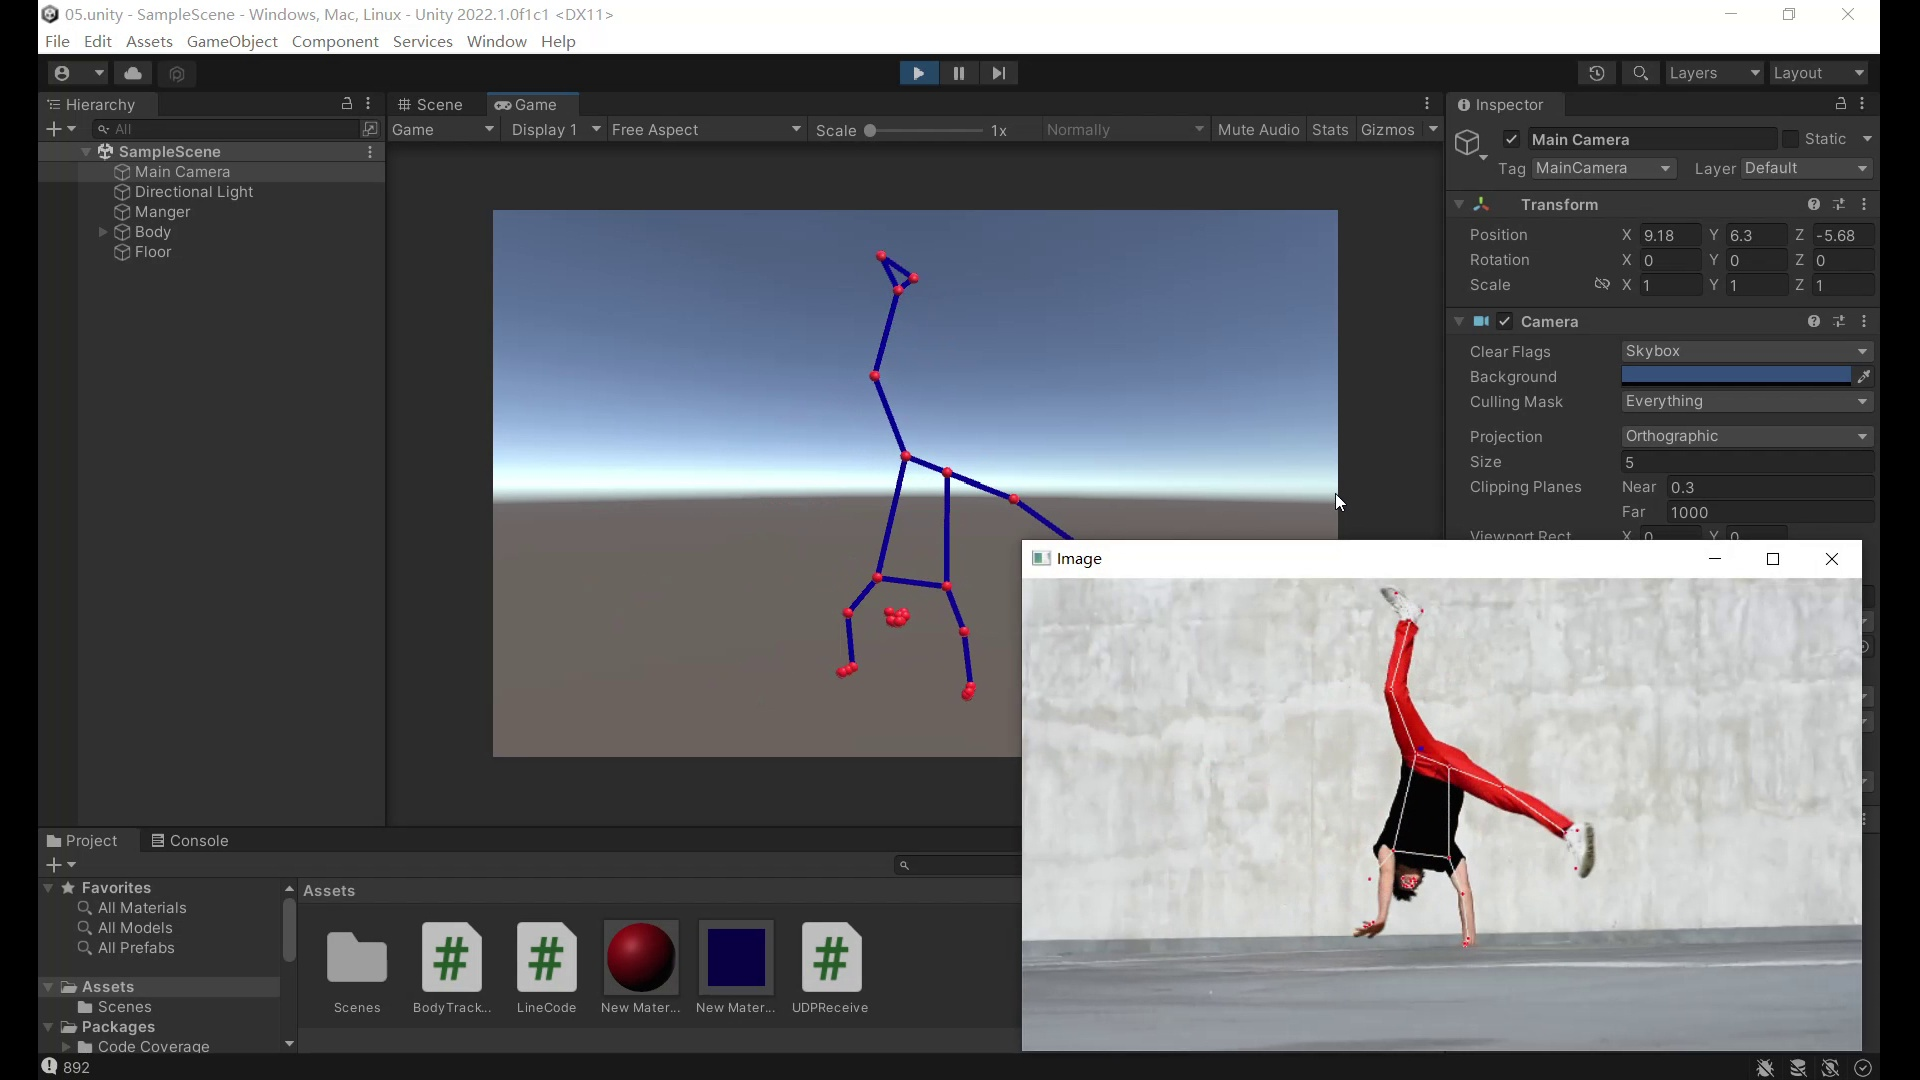
\includegraphics[width=0.24\textwidth]{unity2}}
\subfigure{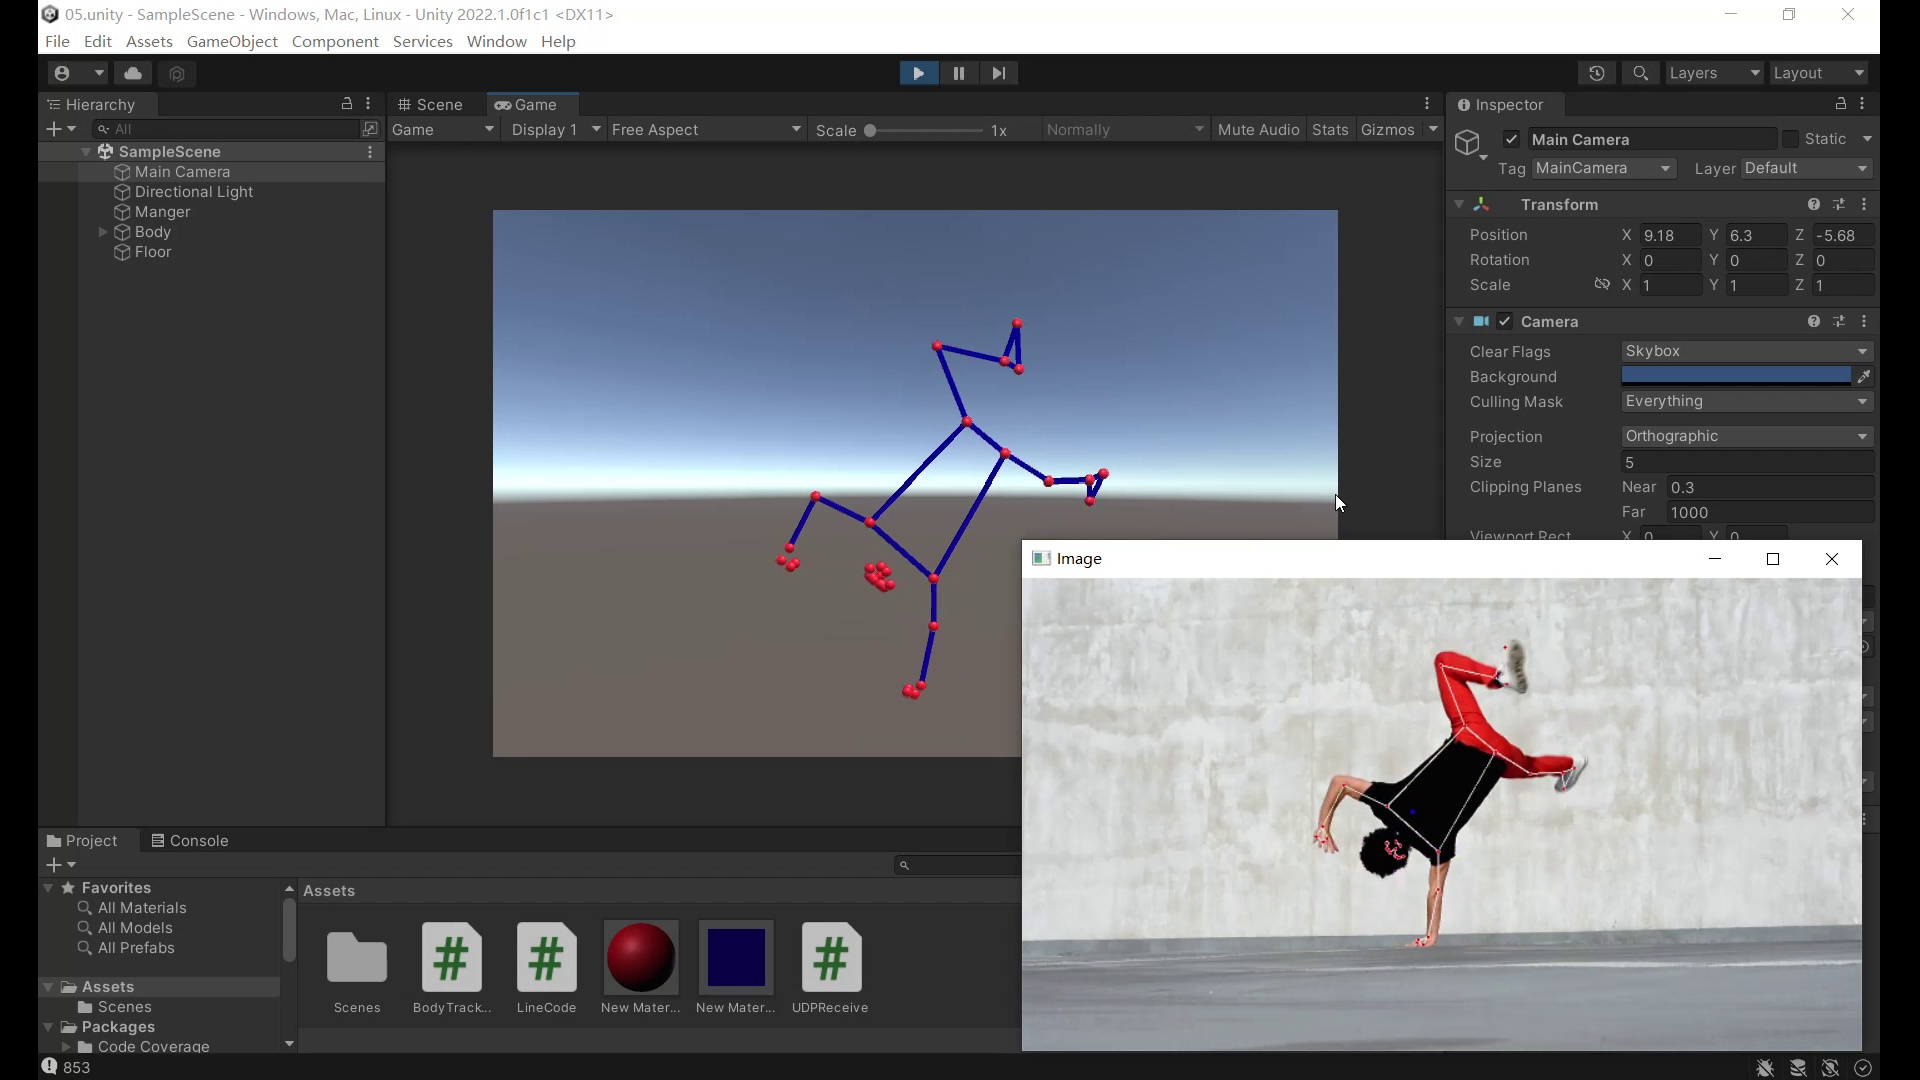
\includegraphics[width=0.24\textwidth]{unity3}}
\subfigure{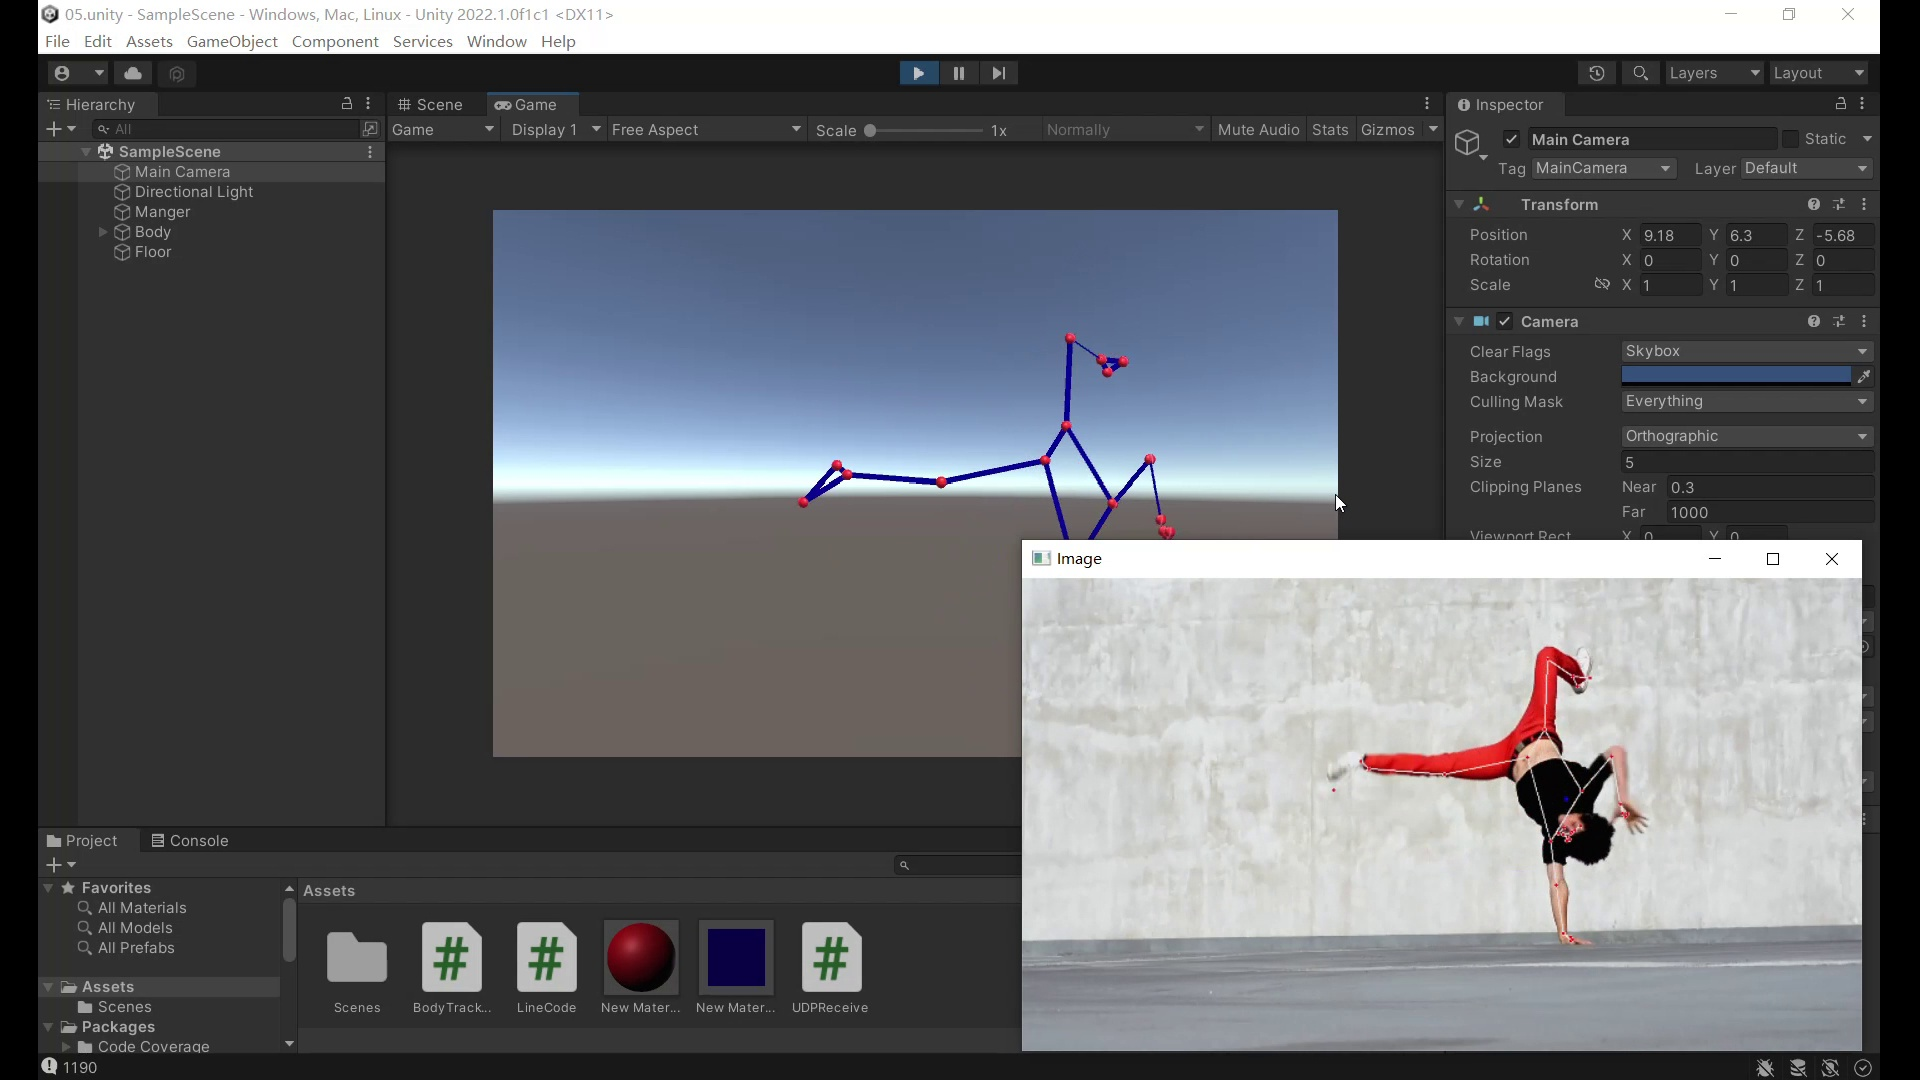
\includegraphics[width=0.24\textwidth]{unity4}}
\end{minipage}
\begin{minipage}{\textwidth}
\centering
\subfigure{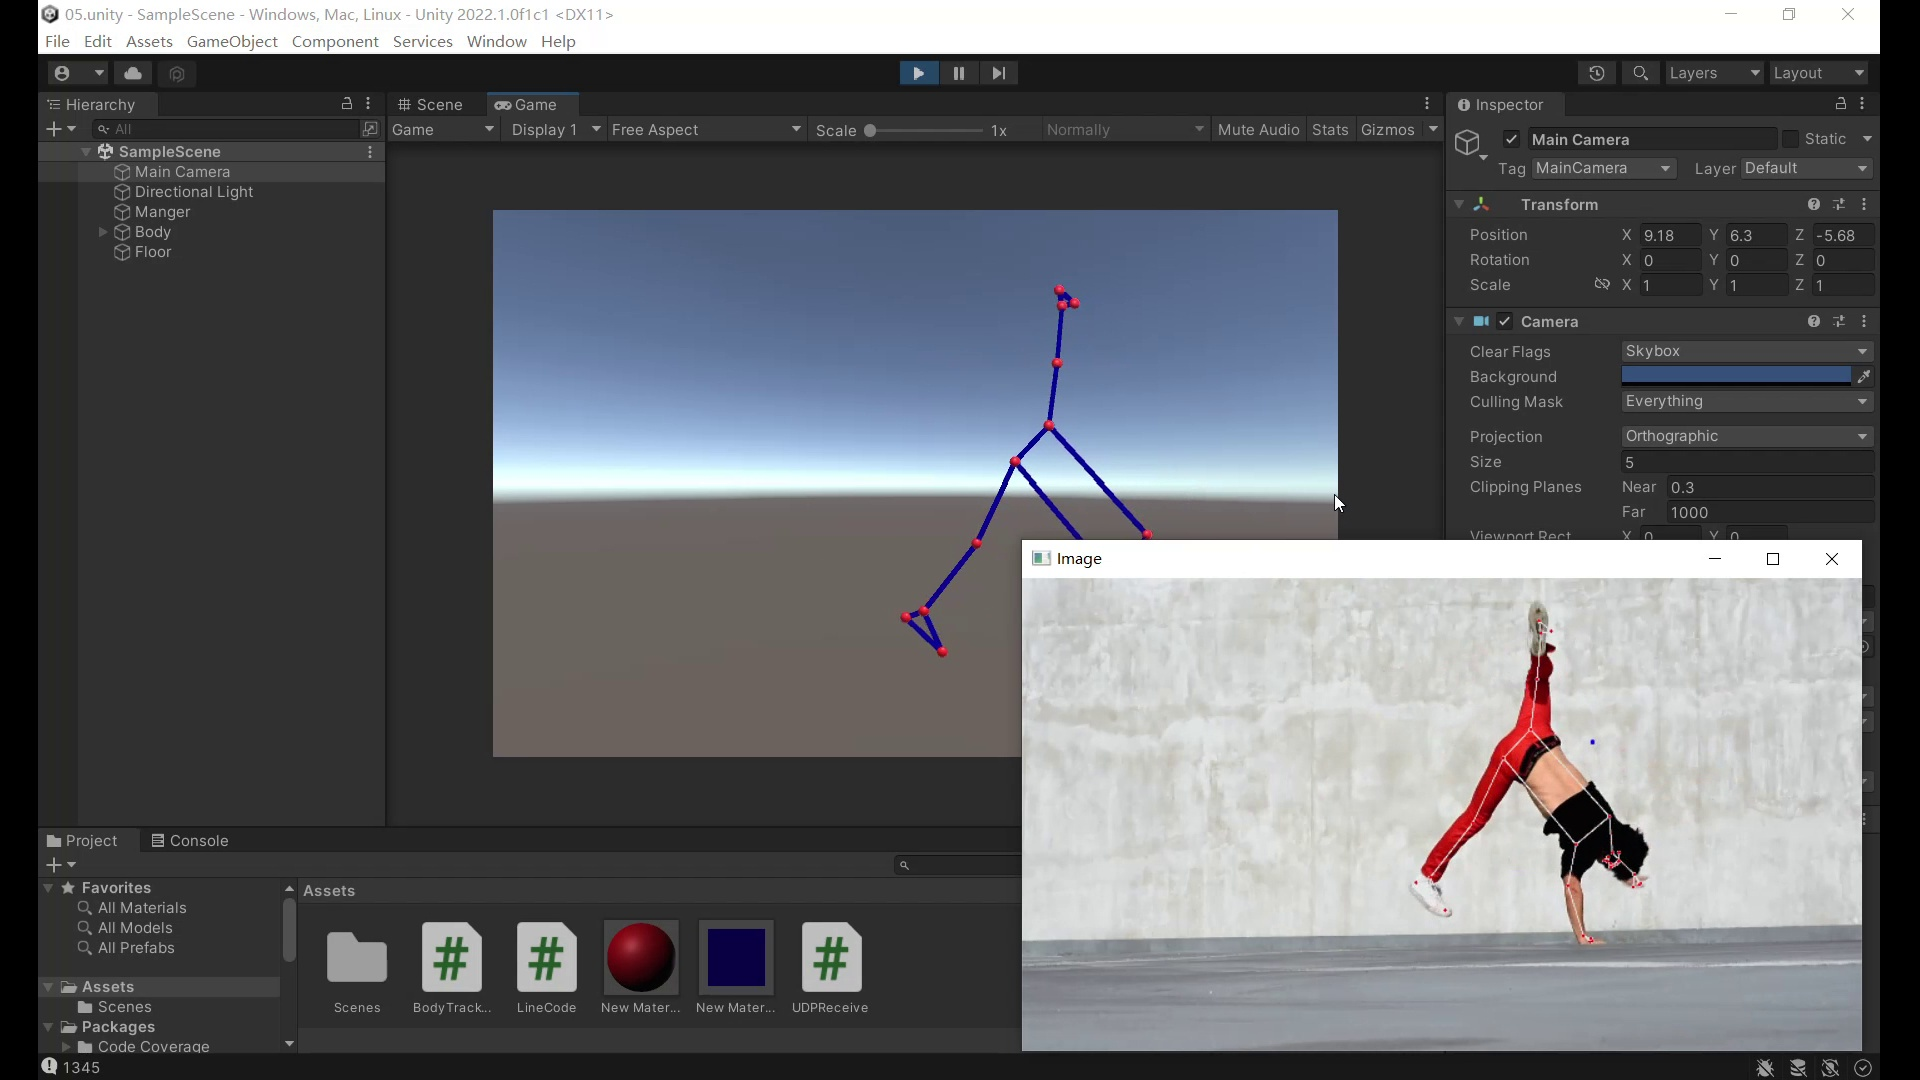
\includegraphics[width=0.24\textwidth]{unity5}}
\subfigure{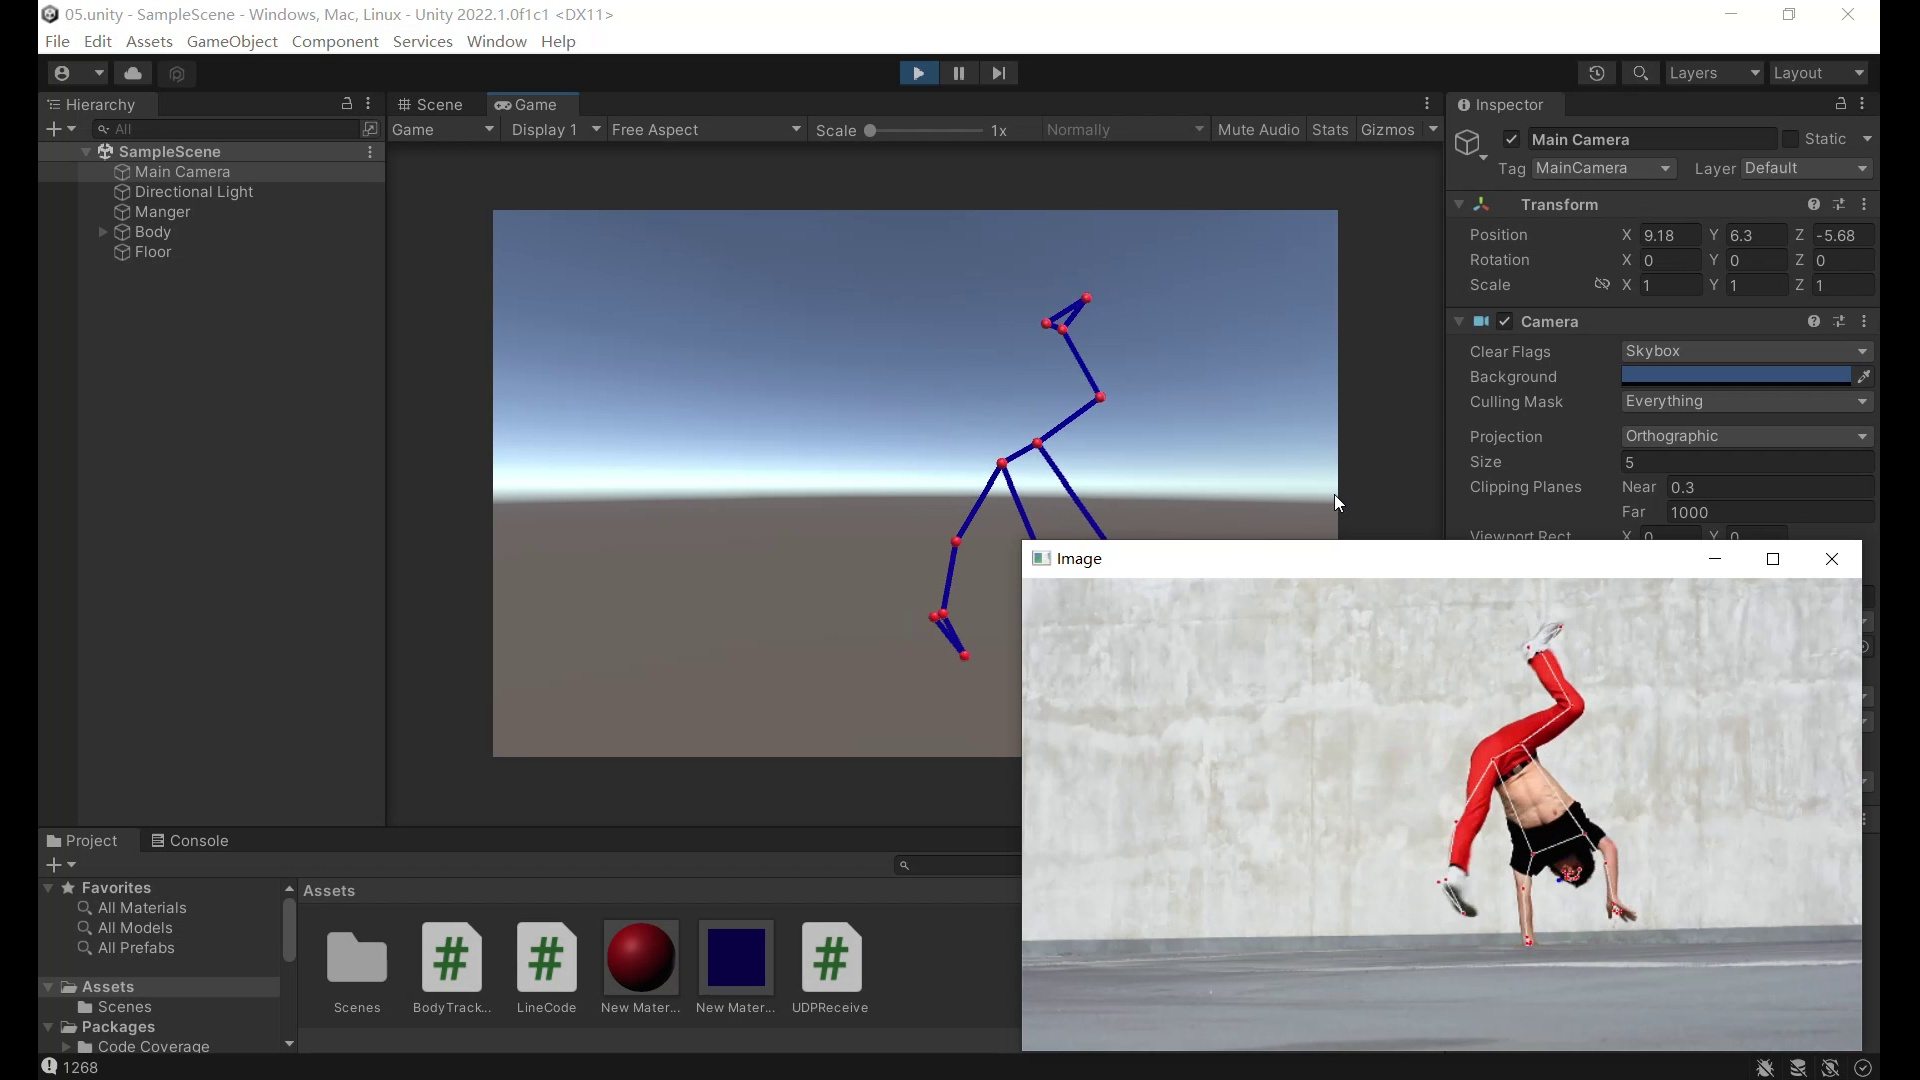
\includegraphics[width=0.24\textwidth]{unity6}}
\subfigure{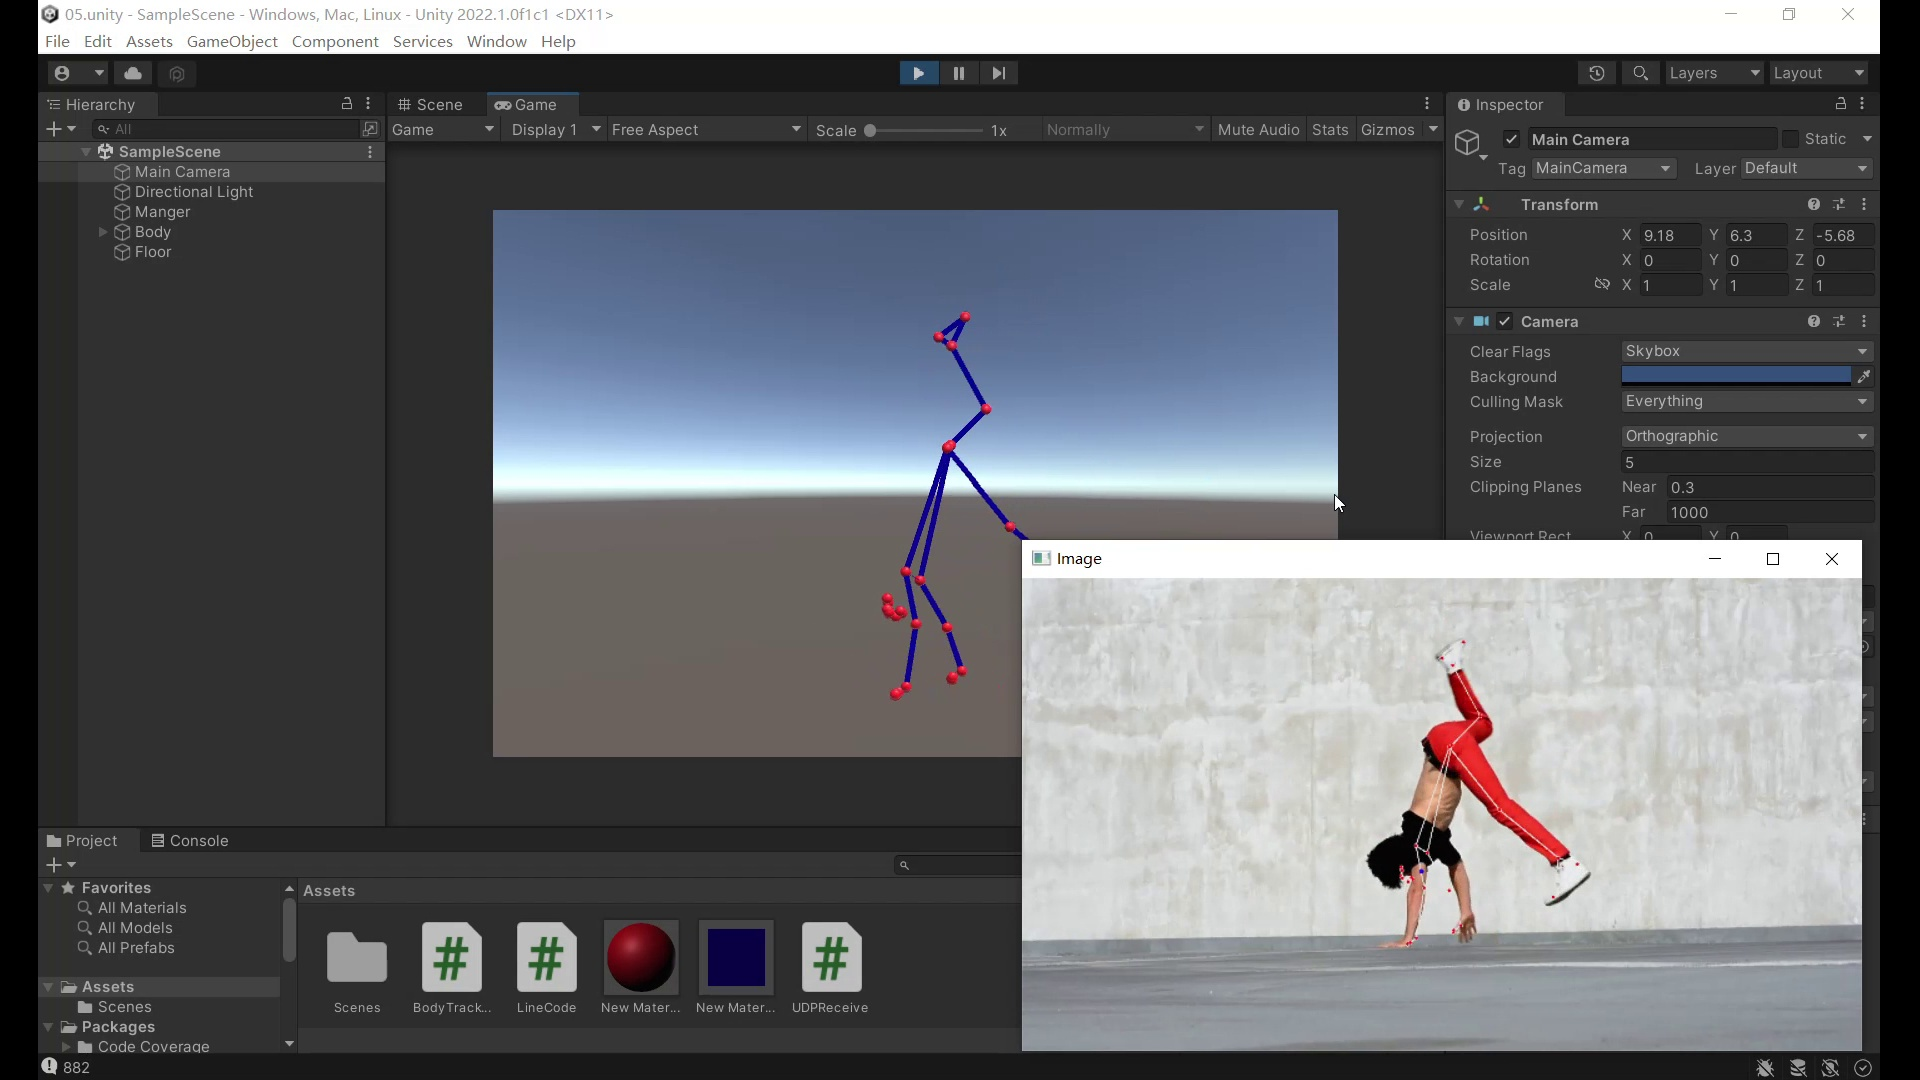
\includegraphics[width=0.24\textwidth]{unity7}}
\subfigure{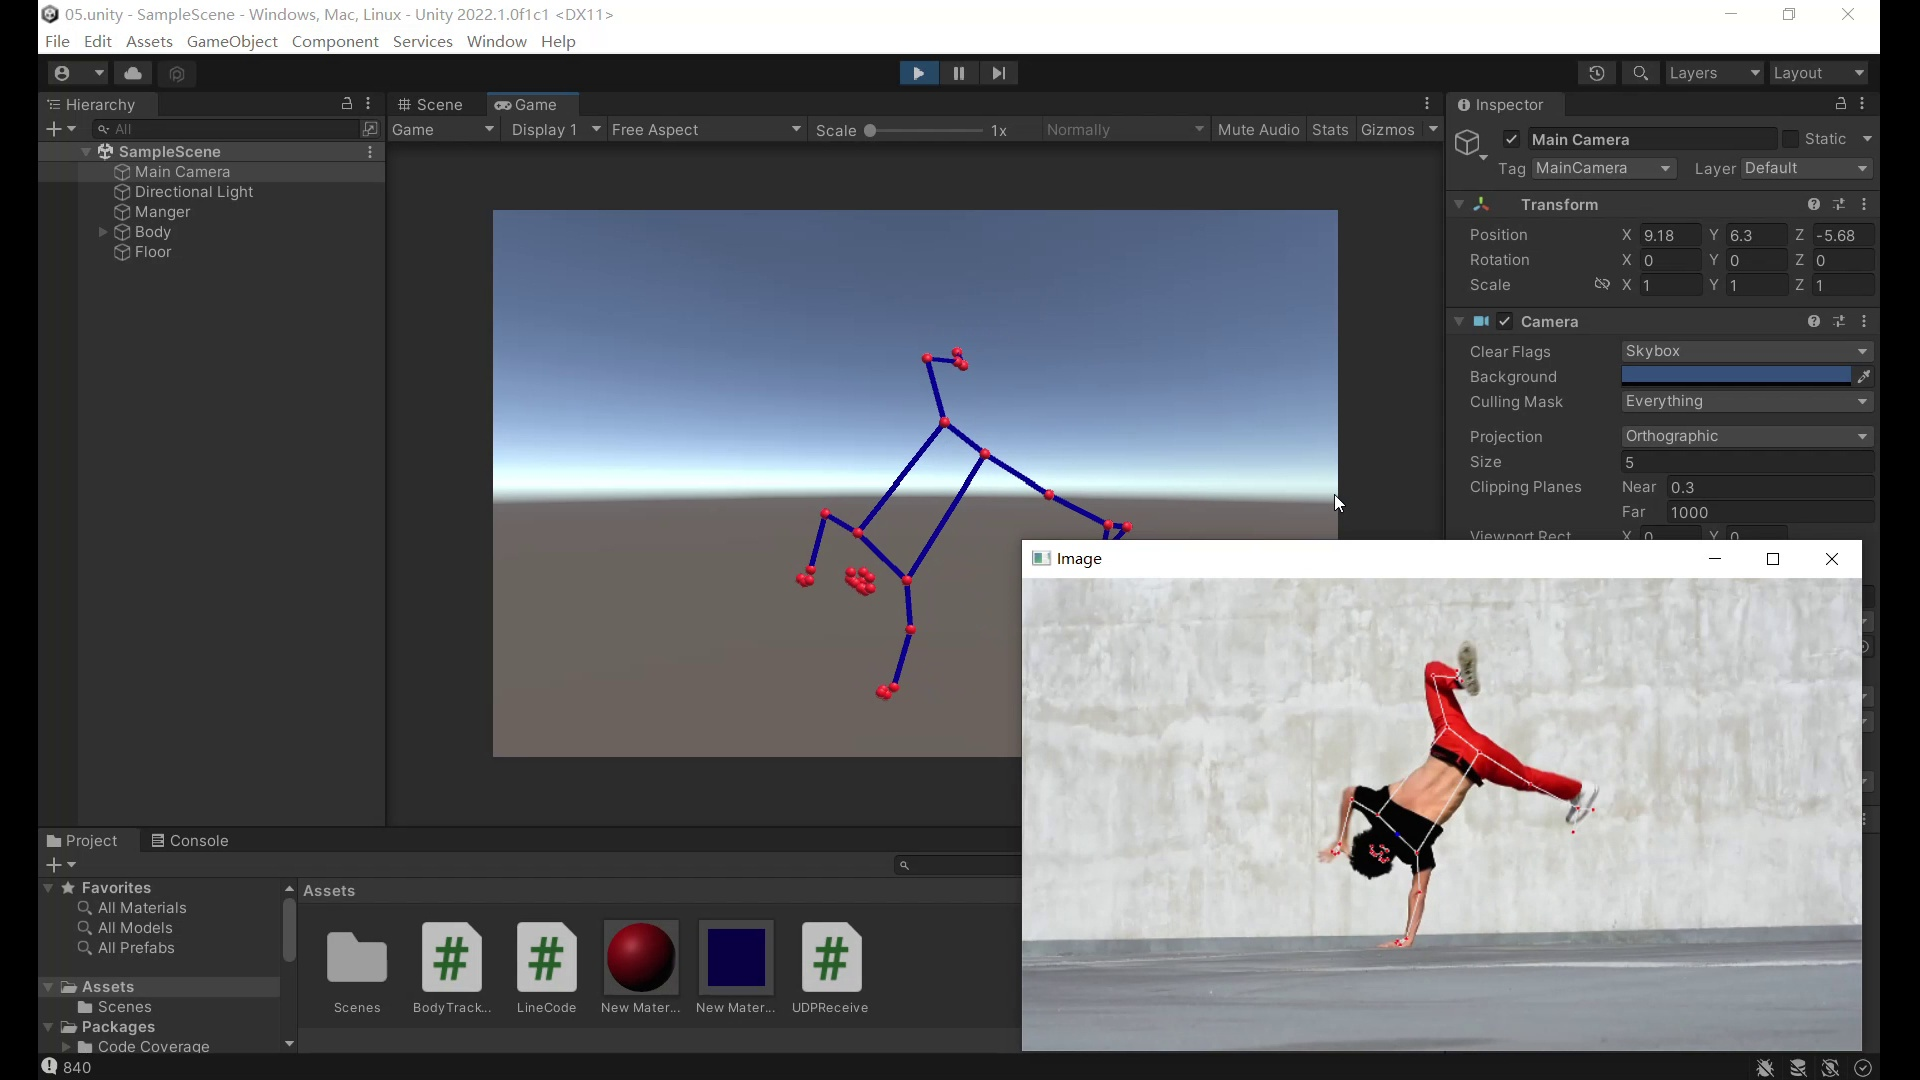
\includegraphics[width=0.24\textwidth]{unity8}}
\end{minipage}
\vspace{0.2em}
\caption{unity虚拟火柴人姿态模仿截图}
\label{picture:24}
\end{figure}

\subsection{真实机器人的姿态模仿}

对于真实机器人,我们使用arduino开发板和SG90舵机来完成实验,arduino开发板指导SG90舵机调整旋转角度,从而达到完成姿态模仿的效果。至于数据传输,我们使用USB串联,主要库为serial。

以右肘部姿态模仿为例,如图~\ref{piture:16}~所示,我们只需计算12-14-16的夹角即可。

记关键点12为$P_1$,关键点14为$P_2$,关键点16为$P_3$,如图~\ref{picture:25}~所示,我们使用math.atan2函数,分别计算出线$P_3P_2$和$X$轴的夹角$\angle P_3P_2X$和线$P_1P_2$和$X$轴的夹角$\angle P_1P_2X$,然后再用$\angle P_3P_2X-\angle P_1P_2X$即可得到$\angle P_1P_2P_3$,即右肘部对应的舵机应该旋转的角度。

计算角度的关键代码如下:

\begin{python}
def findAngle(self, img, p1, p2, p3):
    # Get the landmarks
    x1, y1 = self.lmList[p1][1:3]
    x2, y2 = self.lmList[p2][1:3]
    x3, y3 = self.lmList[p3][1:3]

    # Calculate the Angle
    angle = math.degrees(math.atan2(y3 - y2, x3 - x2) -
                         math.atan2(y1 - y2, x1 - x2))
    if angle < 0:
        angle += 360
	
    return angle
\end{python}

\begin{figure}
\centering
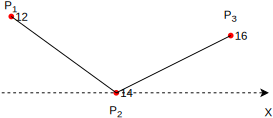
\includegraphics[width=0.9\linewidth]{angle}
\caption{角度计算图示}
\label{picture:25}
\end{figure}

由于经费有限,不失一般性,在本次实验中我们仅以右肘部单节点姿态模仿为例。对于全节点的机器人,我们只需按照单节点同样原理计算出多节点的角度并传到arduino开发板中即可。

最终效果如图~\ref{picture:26}~所示
\begin{figure}[!h]
\setlength{\subfigcapskip}{-1bp}
\centering
\begin{minipage}{\textwidth}
\centering
\subfigure{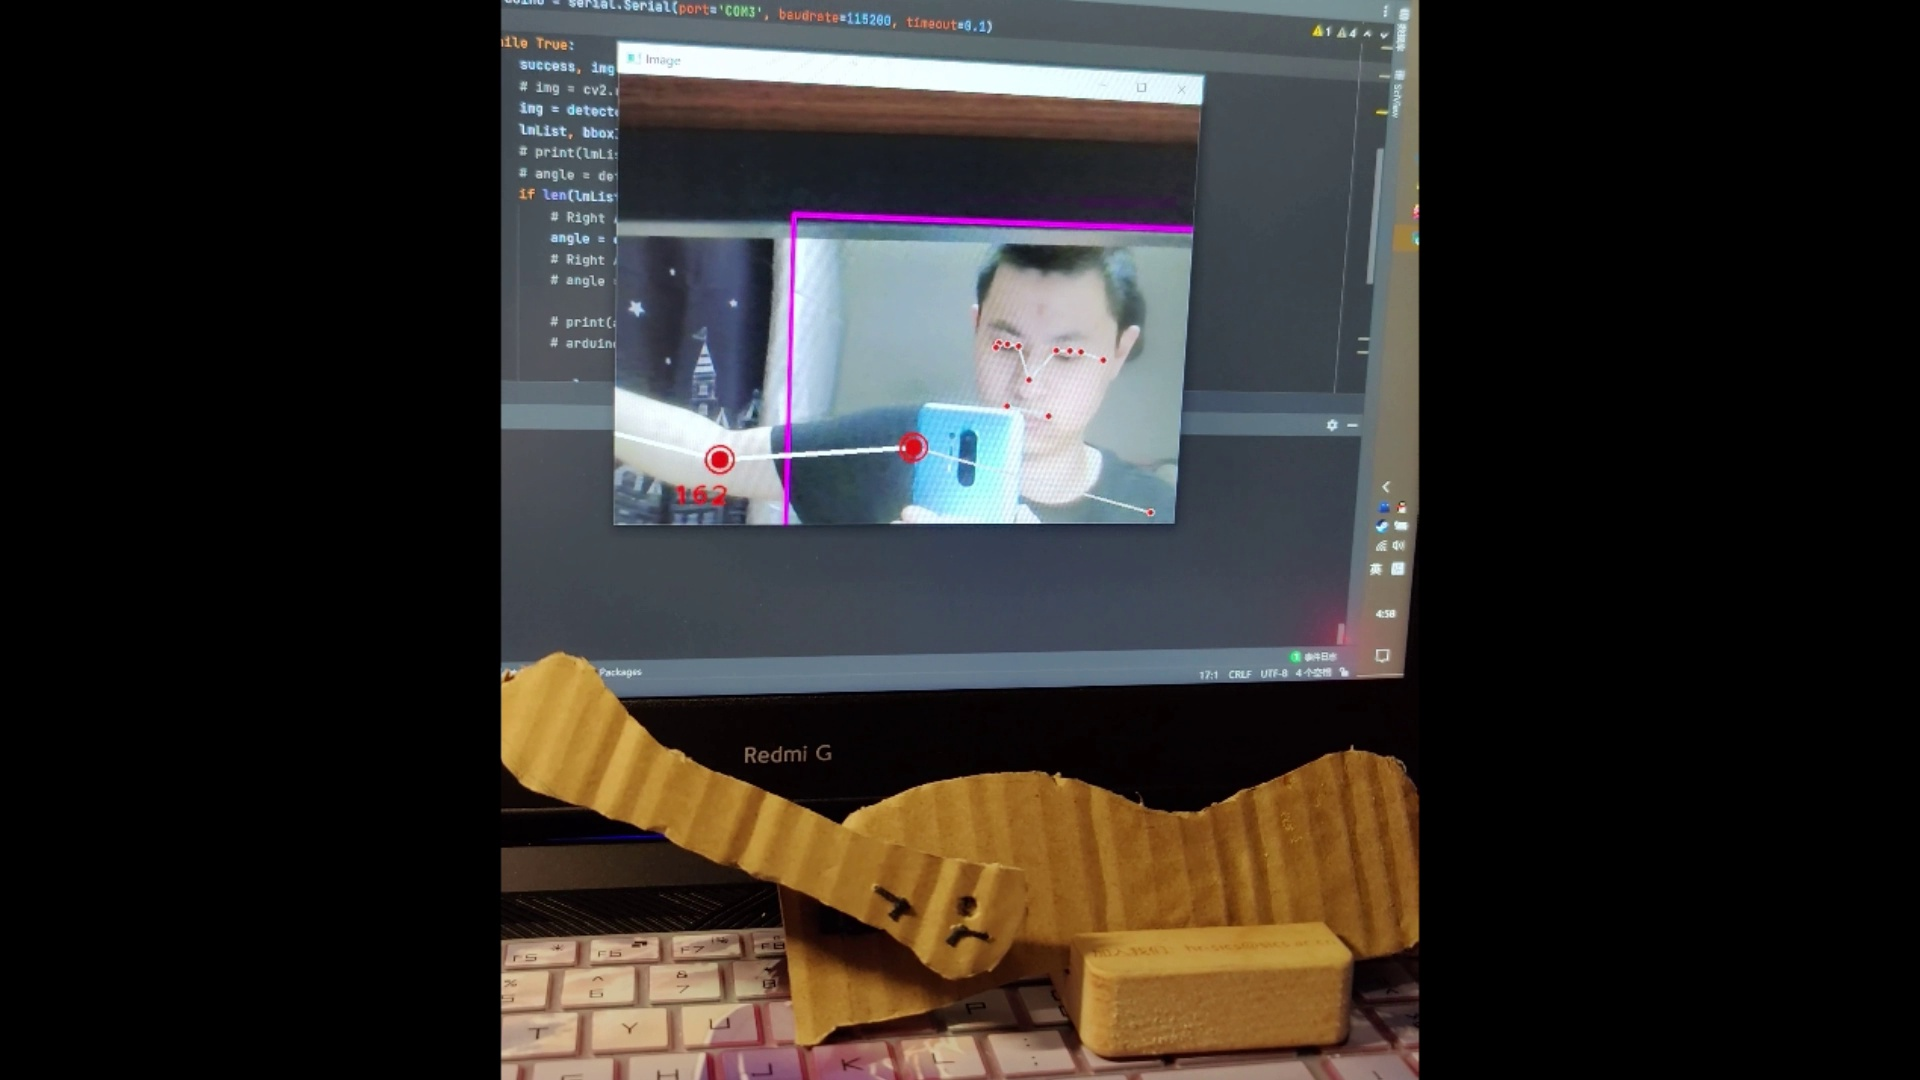
\includegraphics[width=0.31\textwidth]{robot1}}
\subfigure{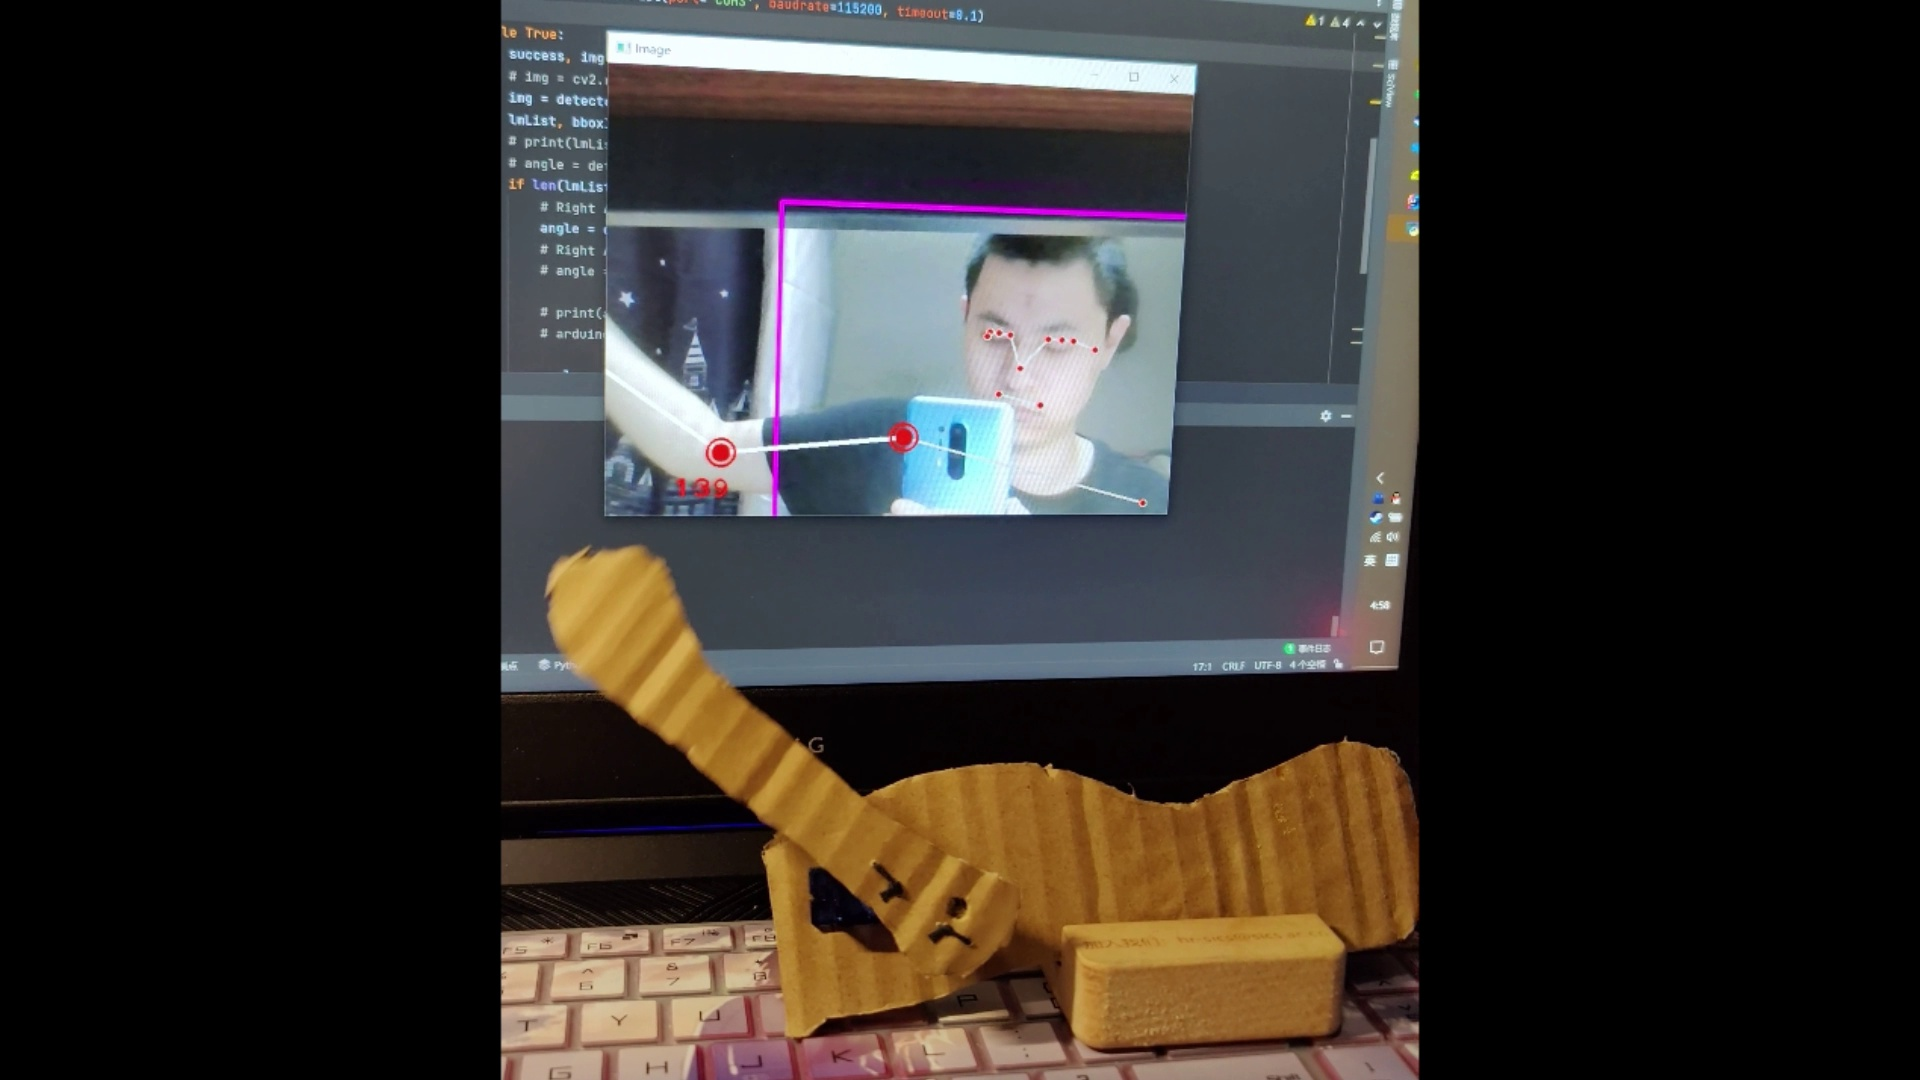
\includegraphics[width=0.31\textwidth]{robot2}}
\subfigure{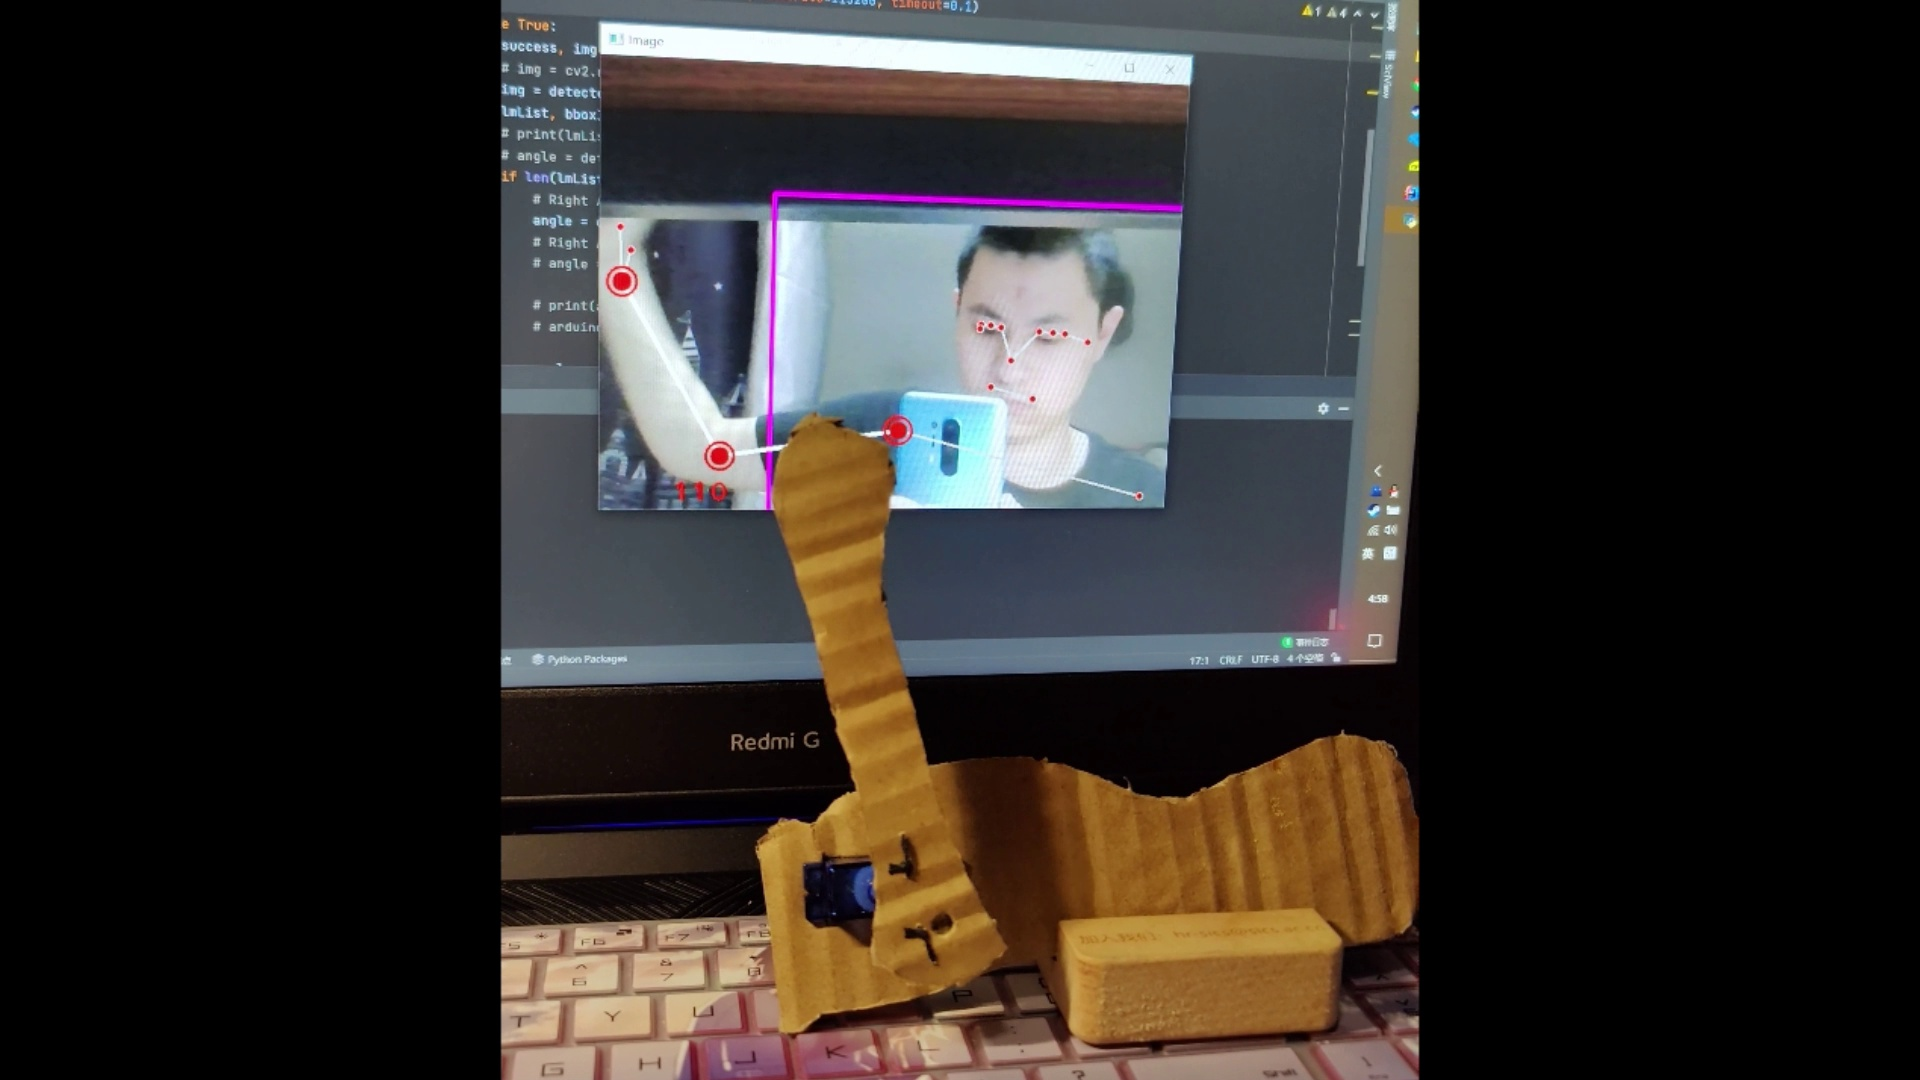
\includegraphics[width=0.31\textwidth]{robot3}}
\end{minipage}
\begin{minipage}{\textwidth}
\centering
\subfigure{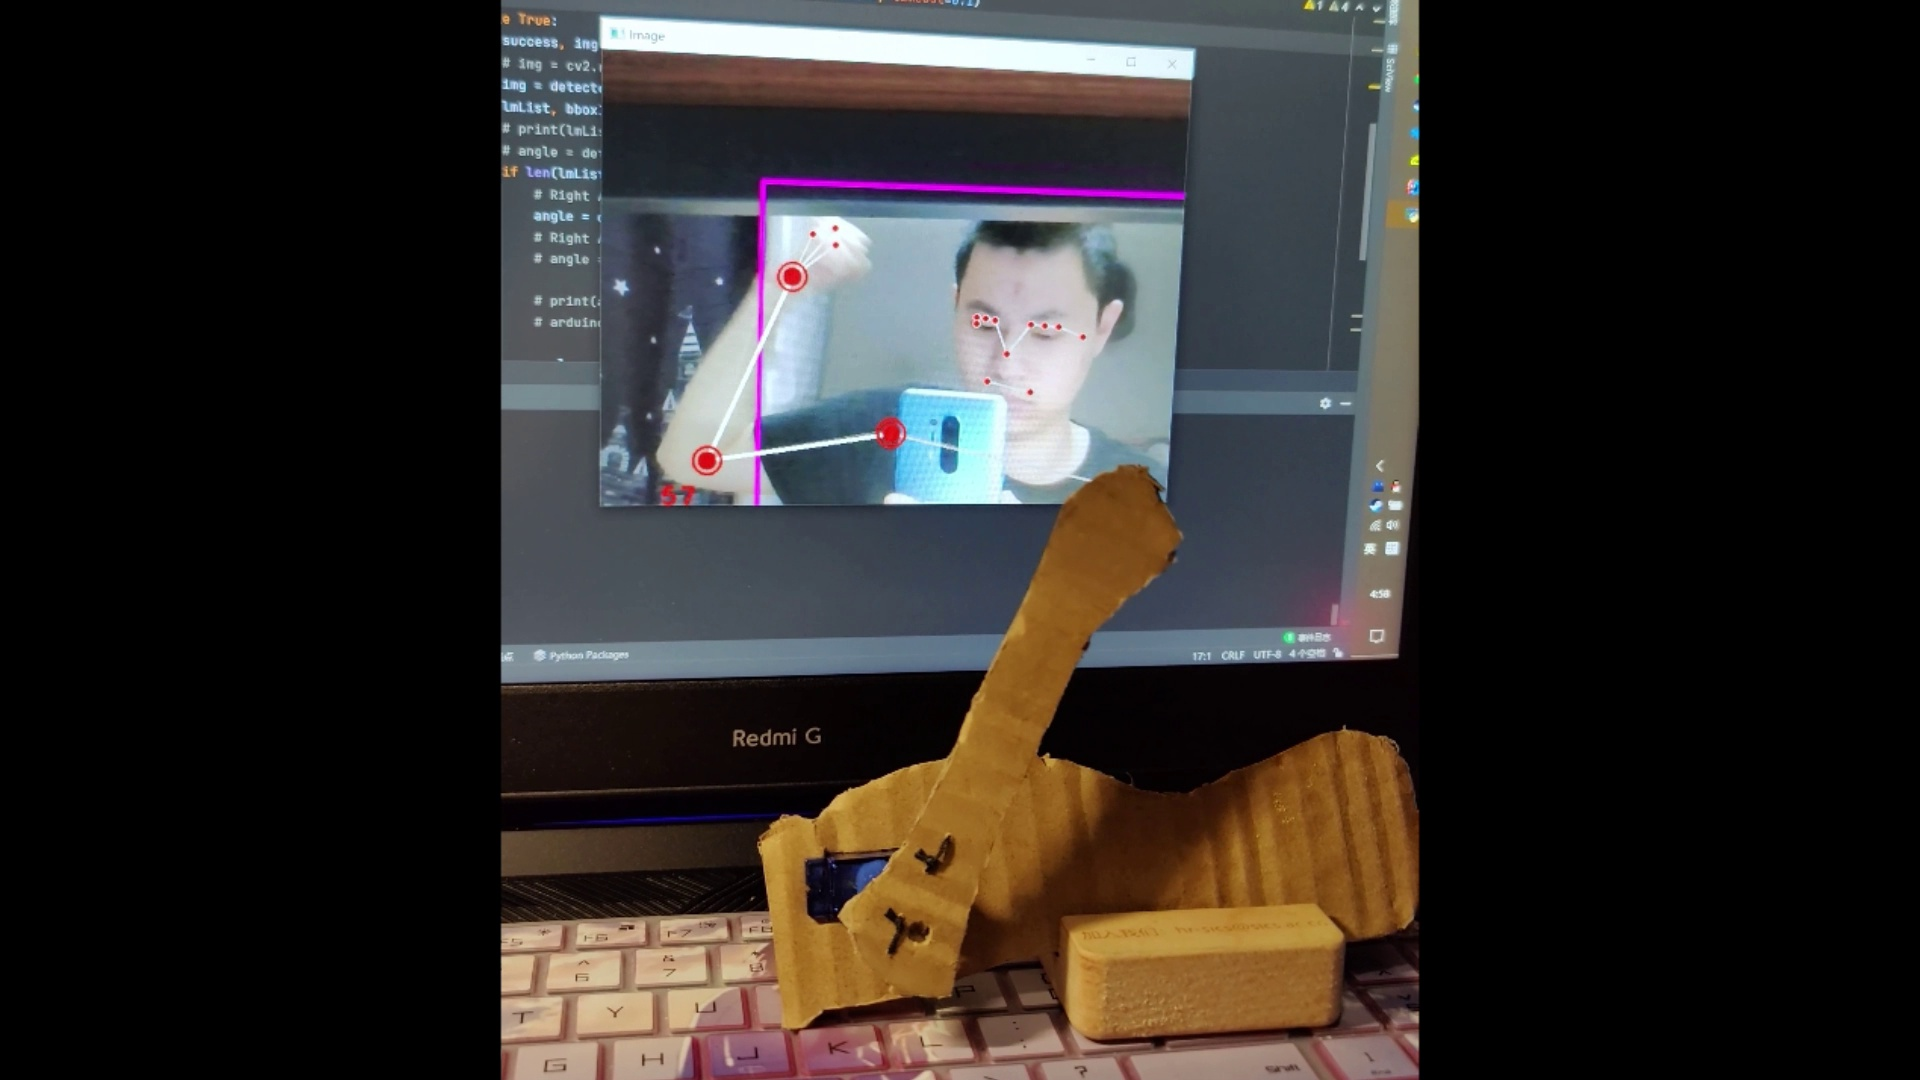
\includegraphics[width=0.31\textwidth]{robot4}}
\subfigure{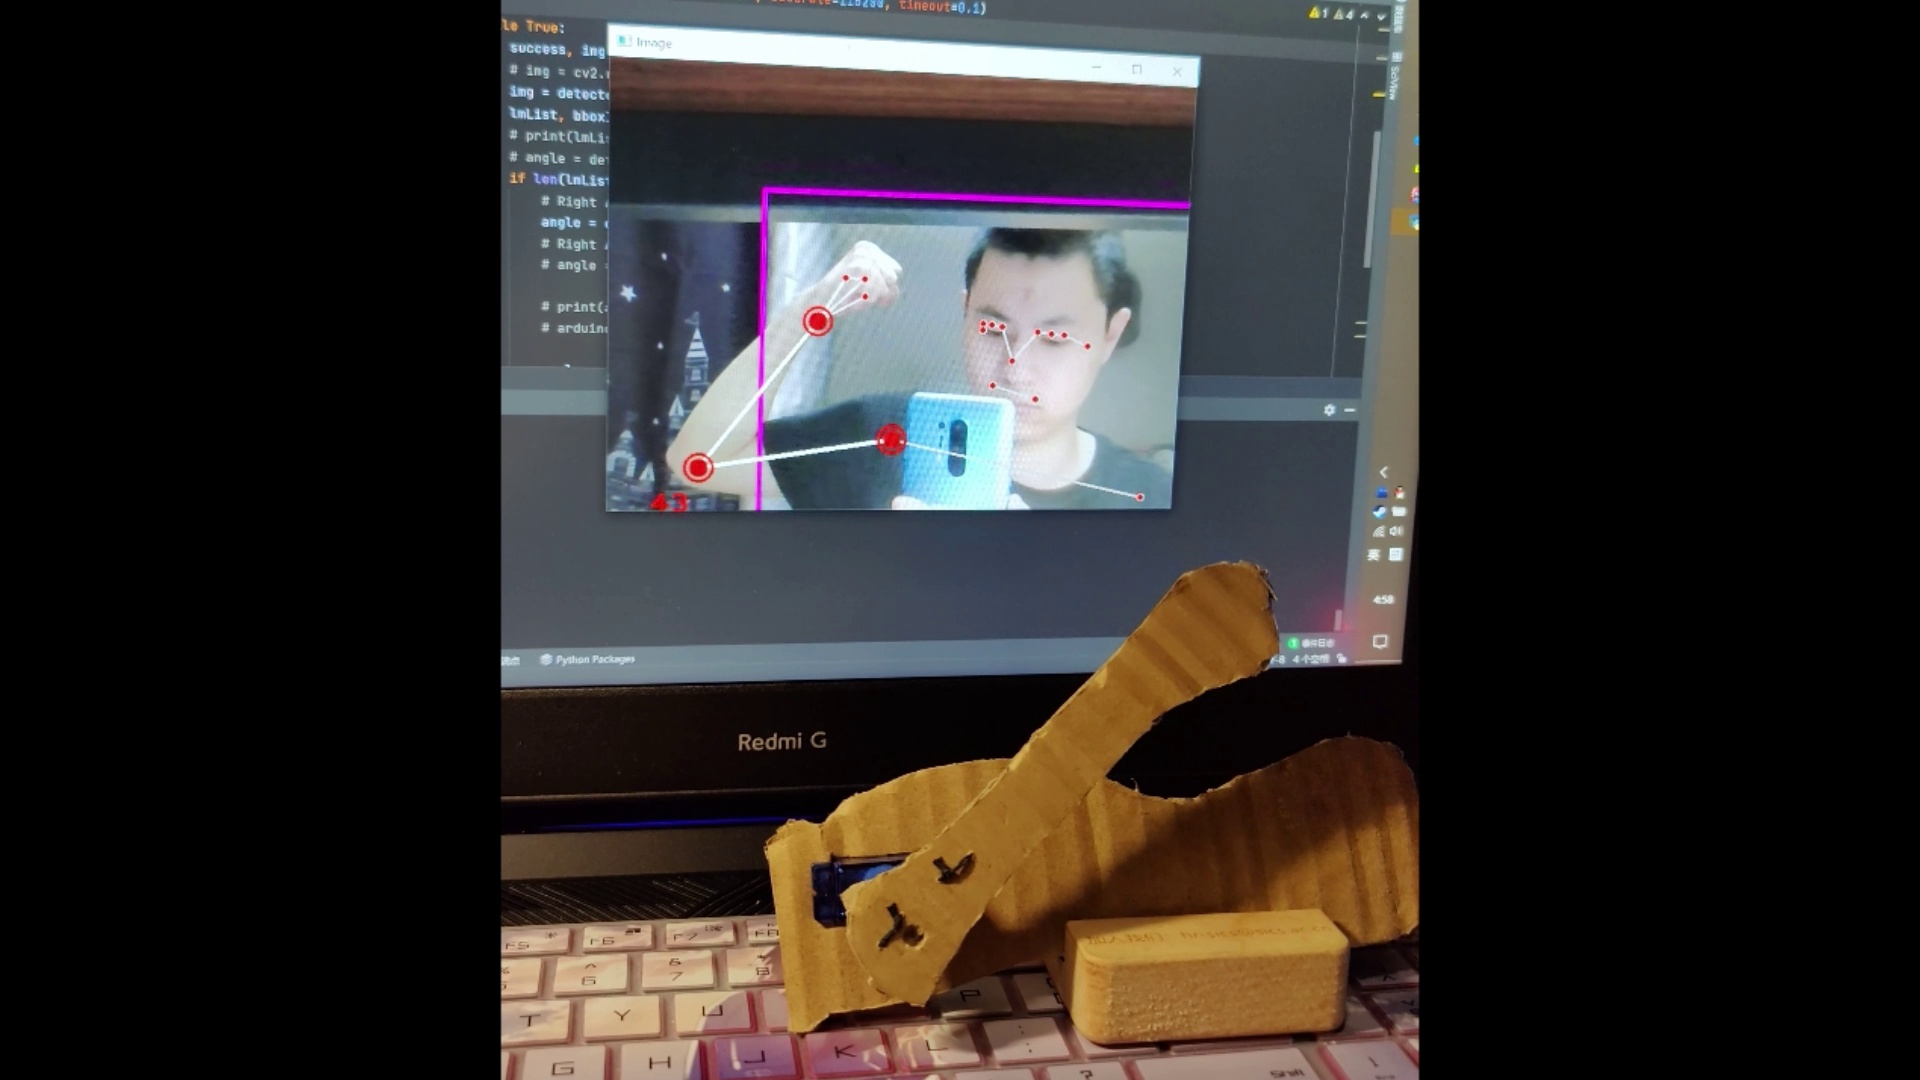
\includegraphics[width=0.31\textwidth]{robot5}}
\subfigure{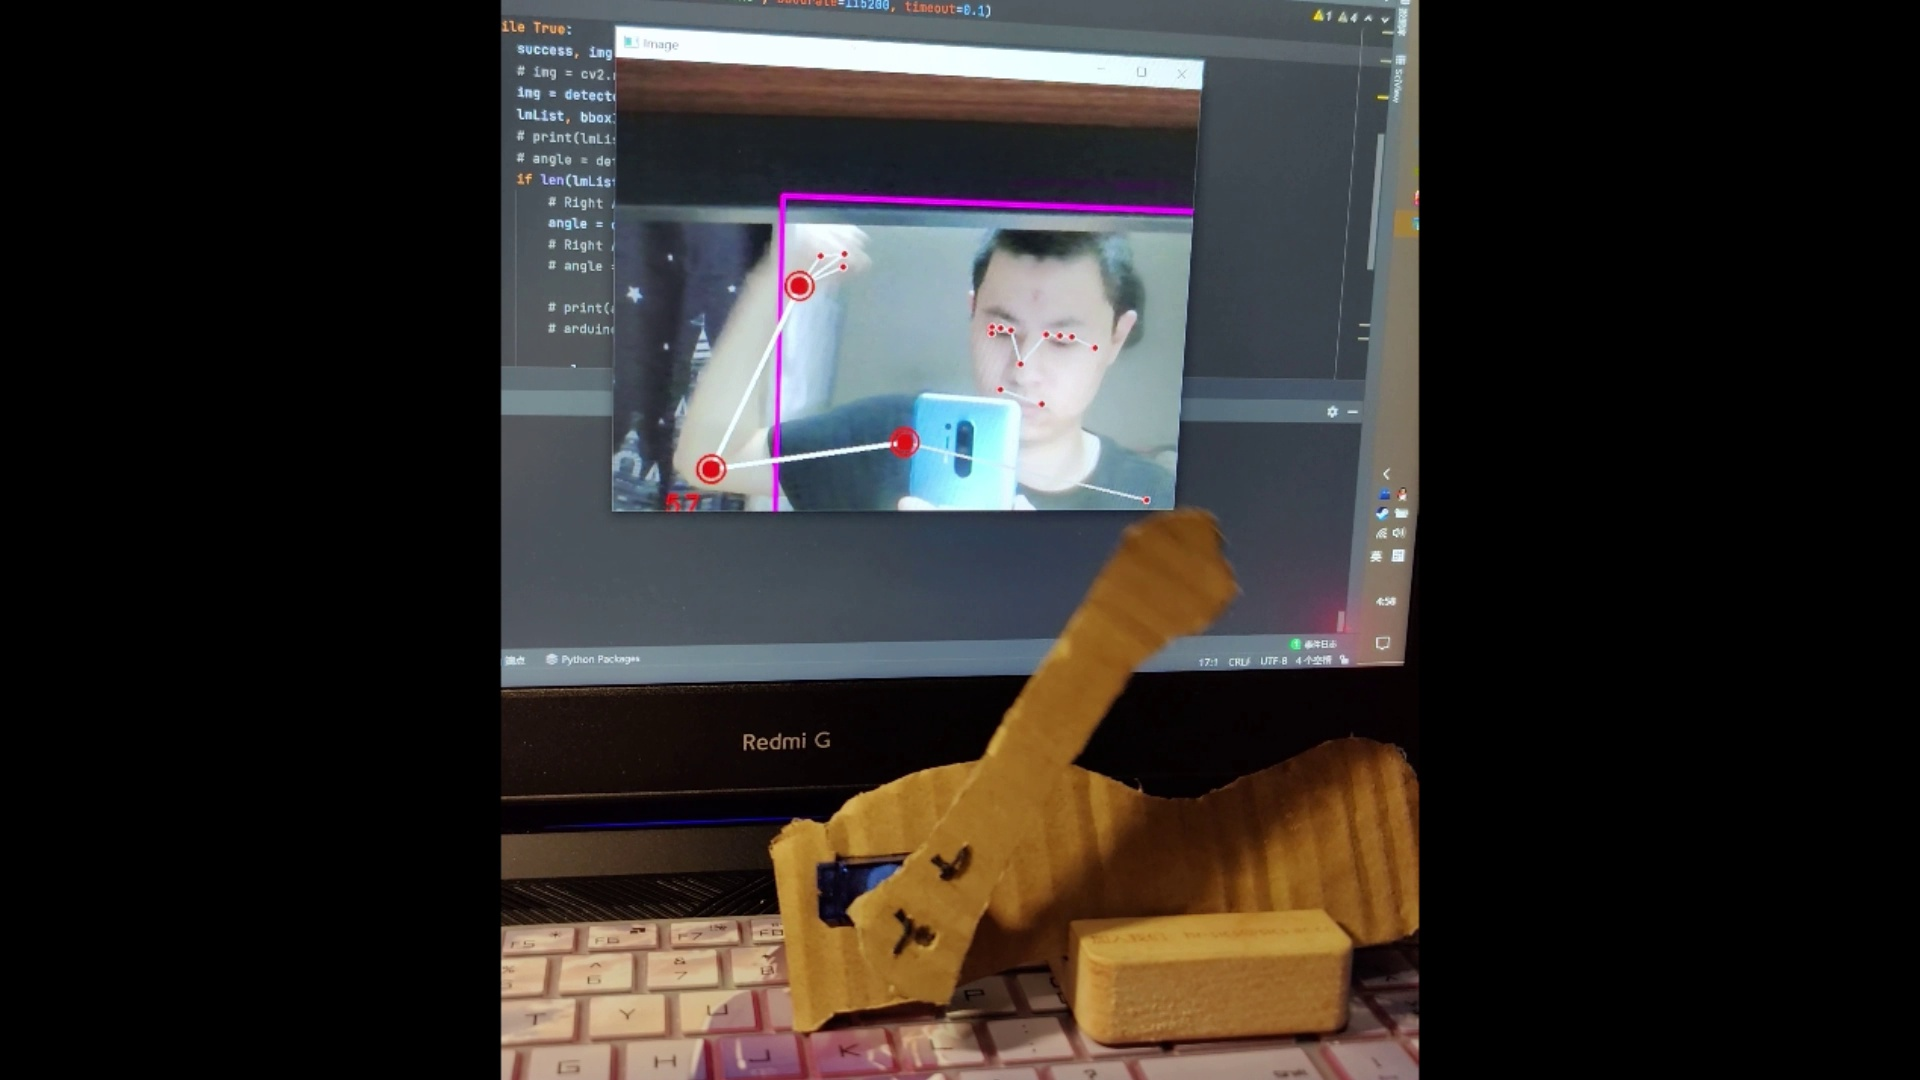
\includegraphics[width=0.31\textwidth]{robot6}}
\end{minipage}
\begin{minipage}{\textwidth}
\centering
\subfigure{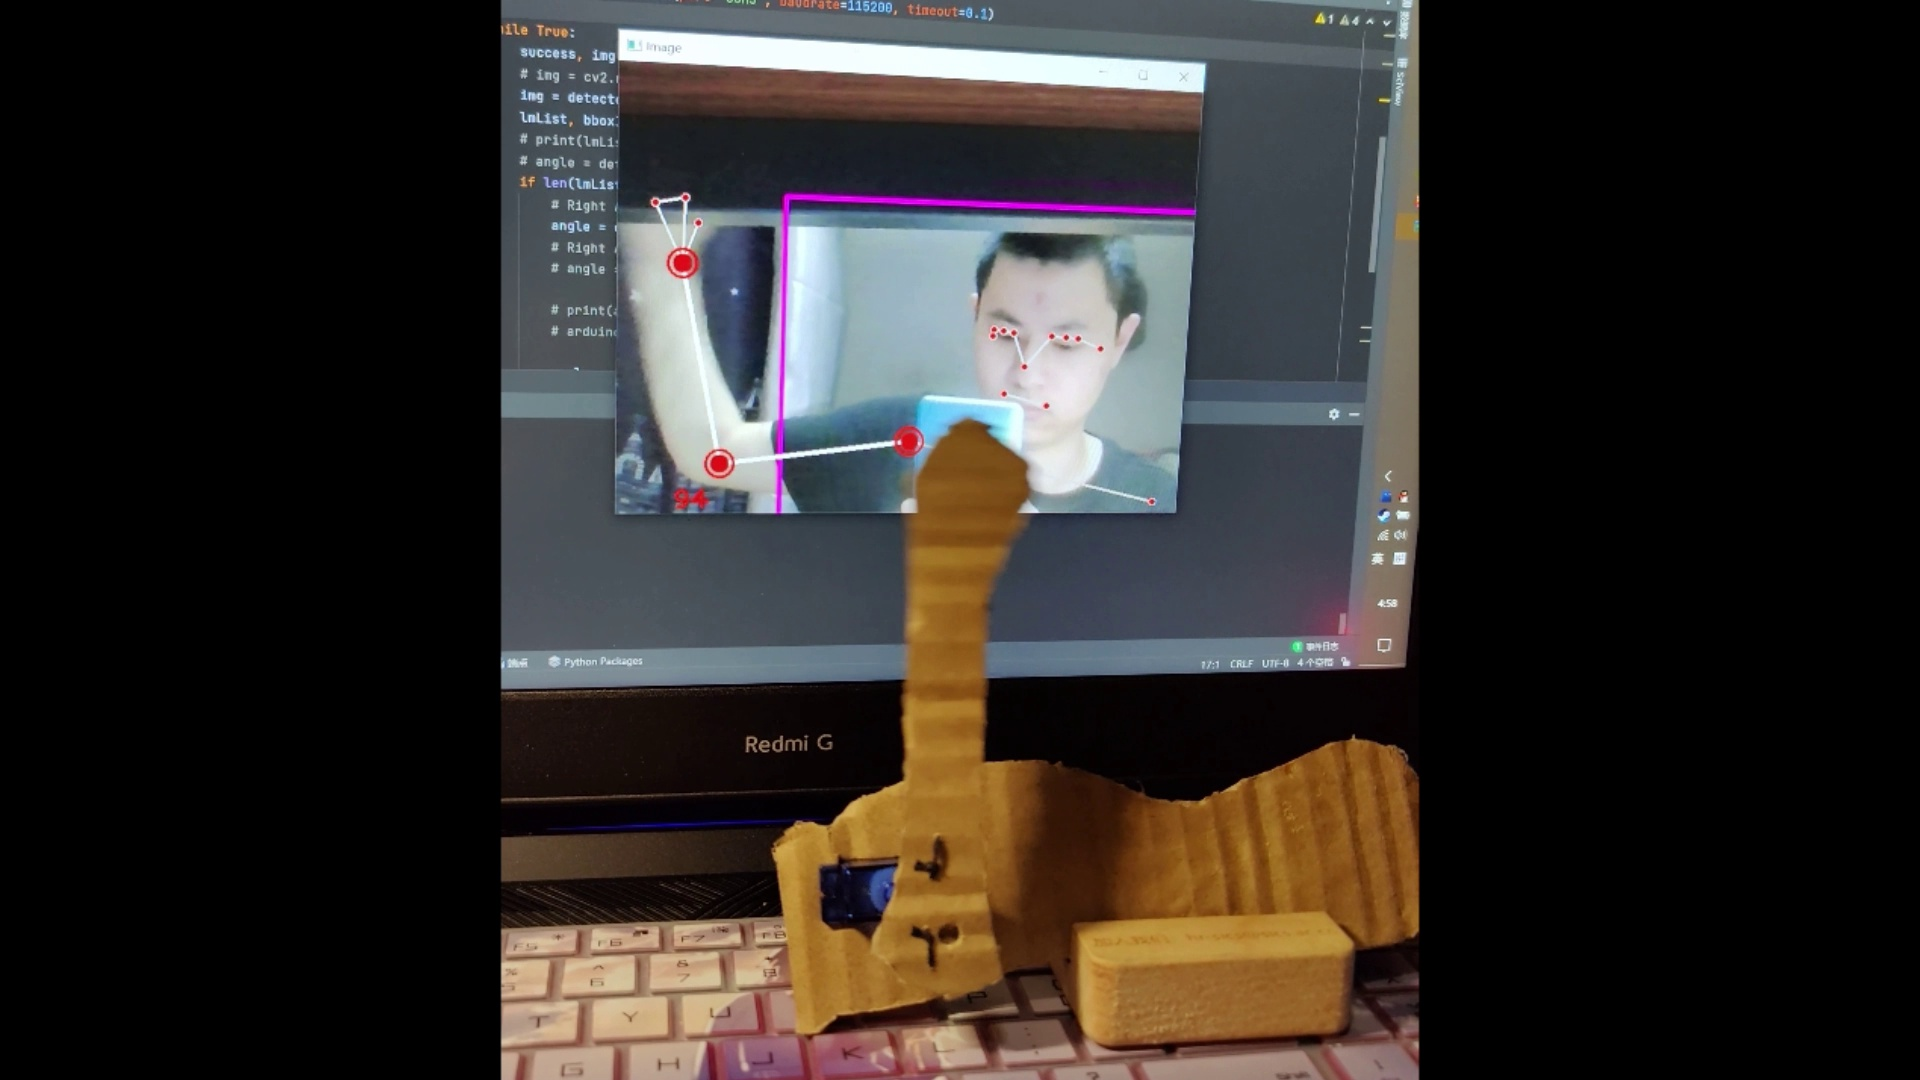
\includegraphics[width=0.31\textwidth]{robot7}}
\subfigure{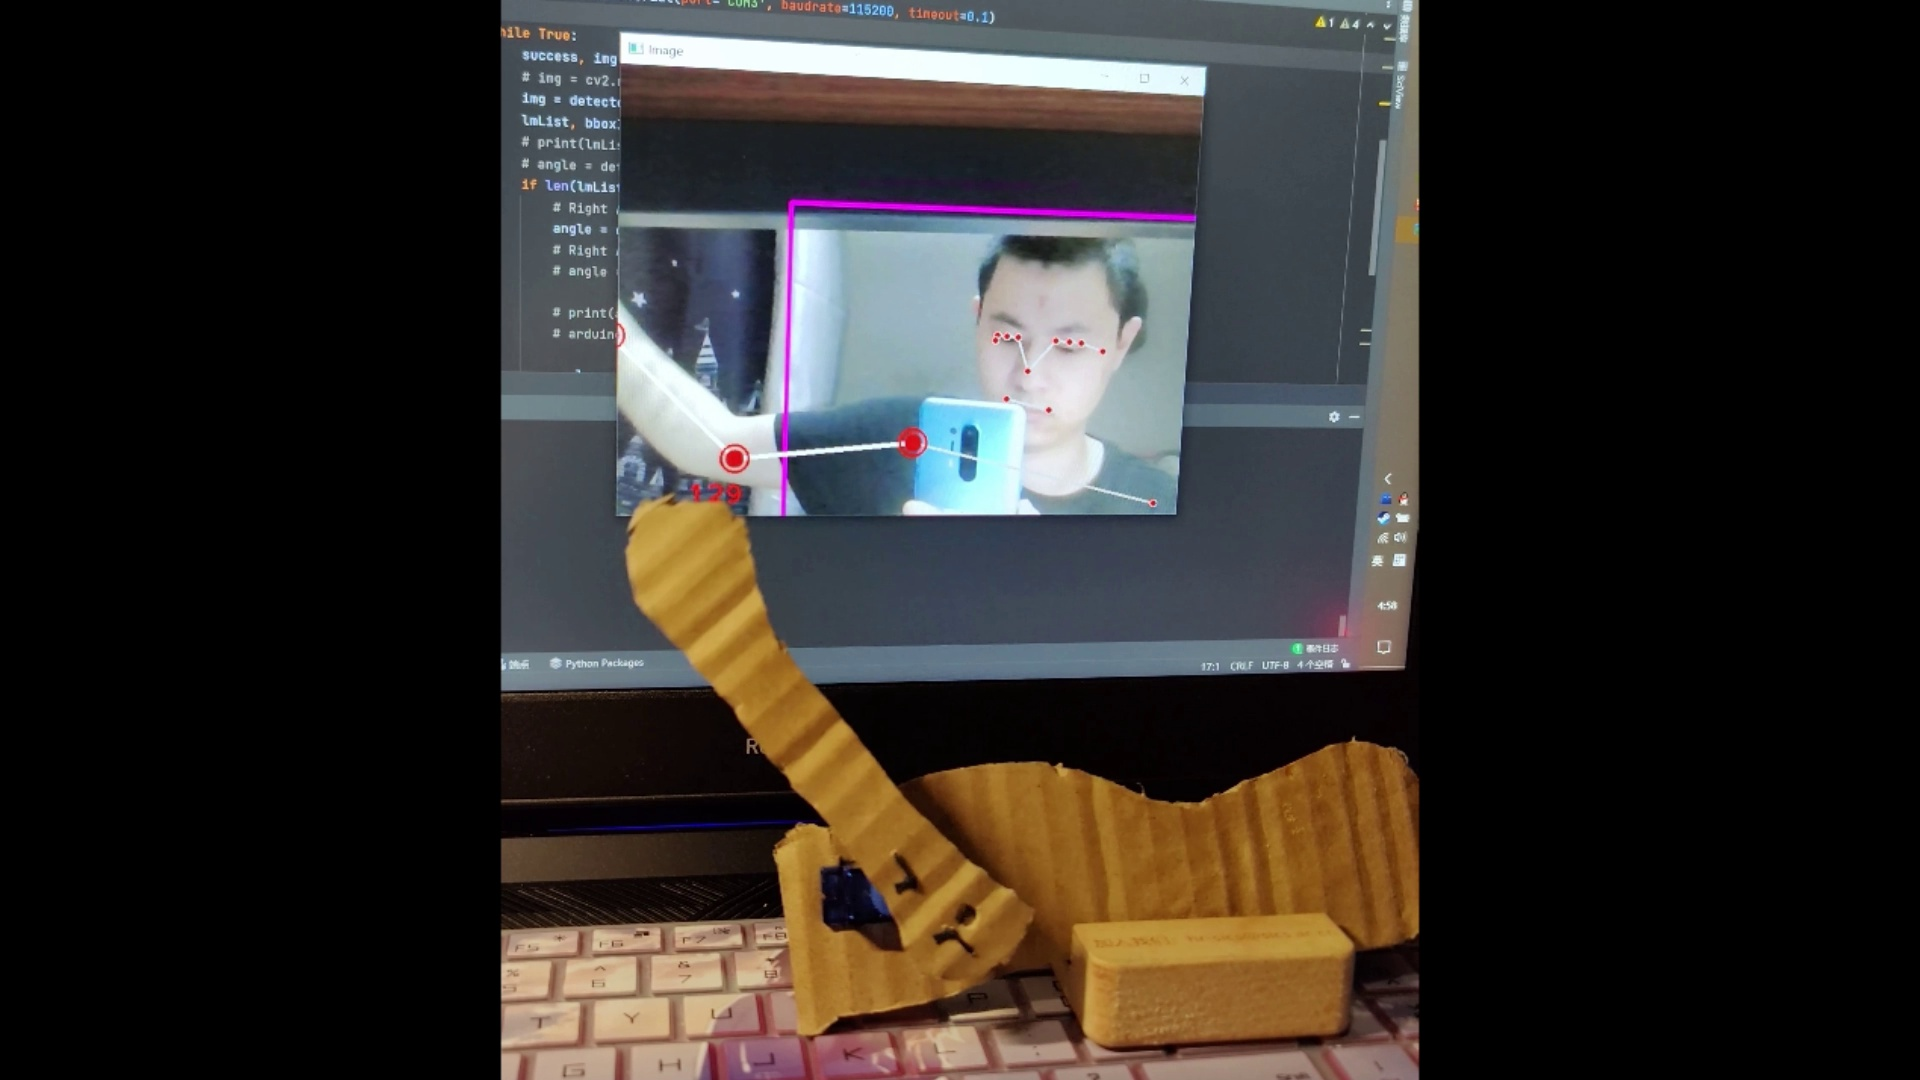
\includegraphics[width=0.31\textwidth]{robot8}}
\subfigure{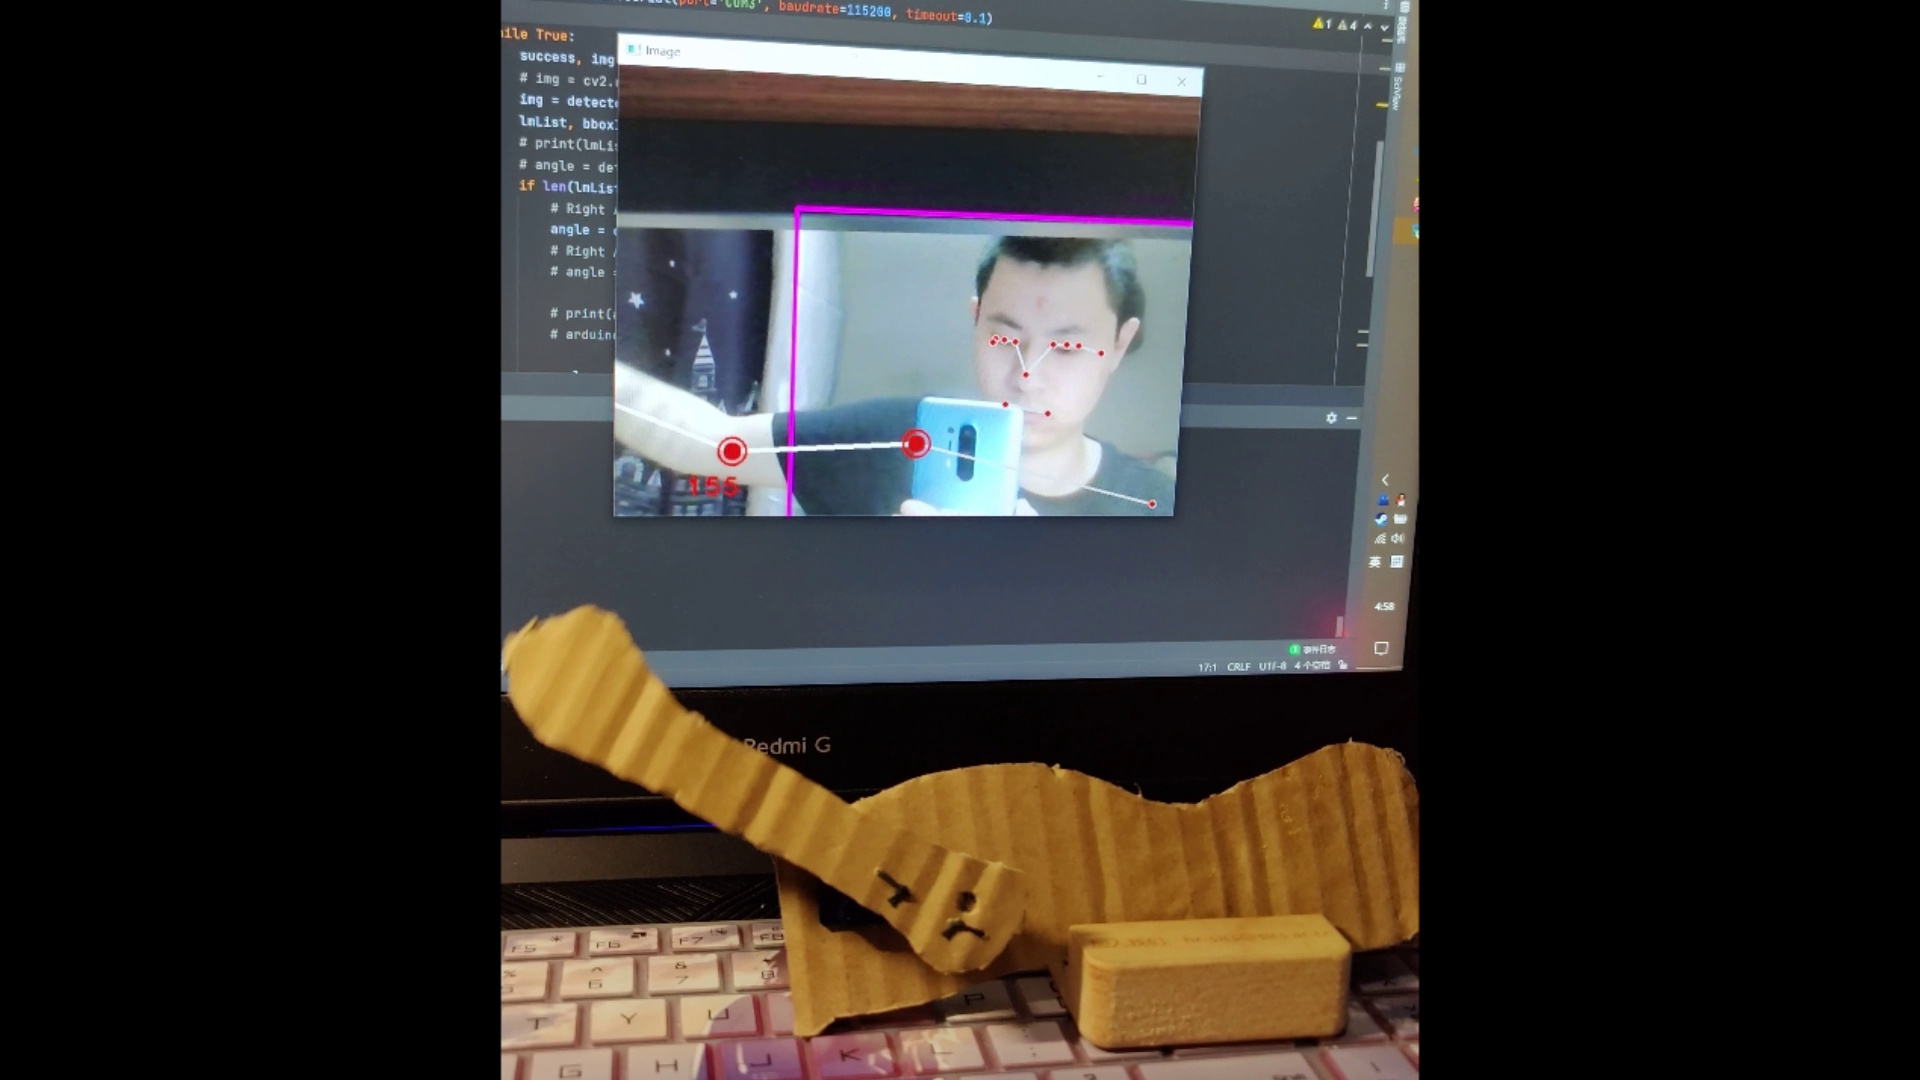
\includegraphics[width=0.31\textwidth]{robot9}}
\end{minipage}
\begin{minipage}{\textwidth}
\centering

\subfigure{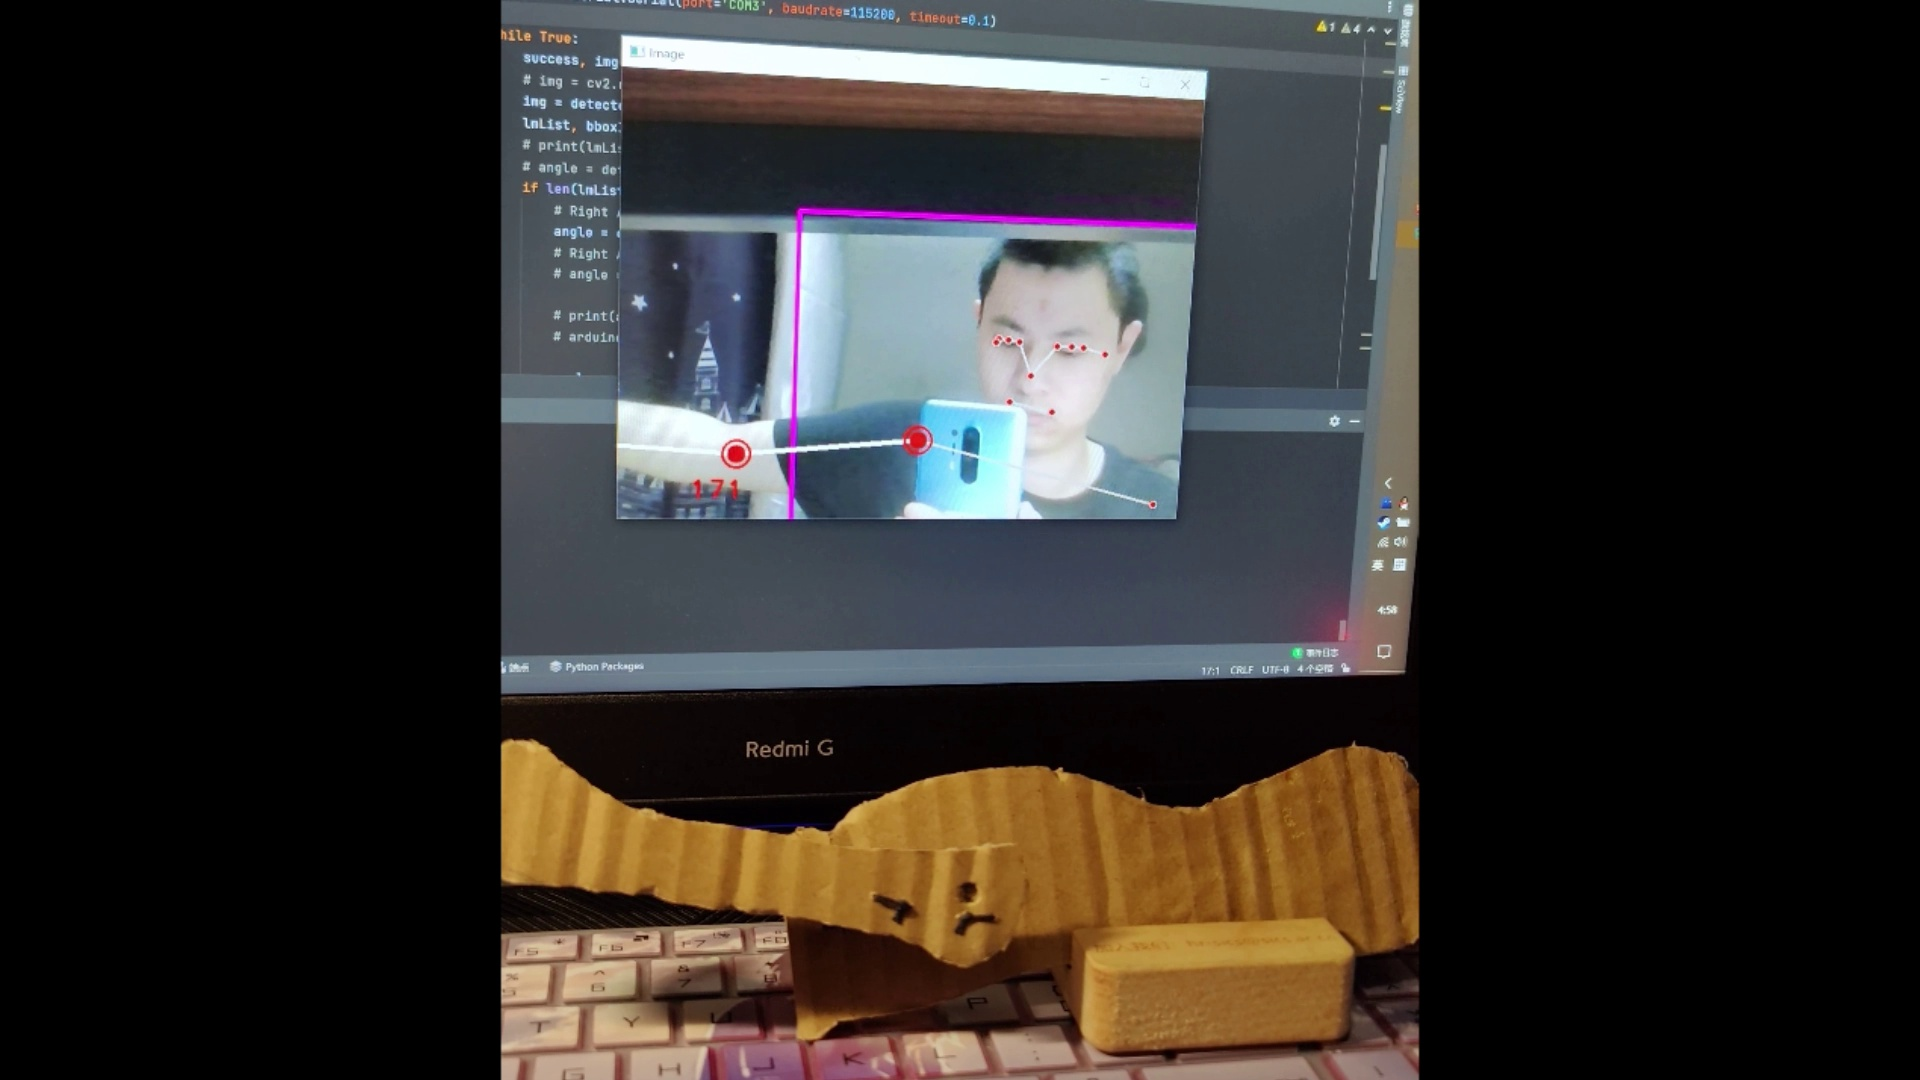
\includegraphics[width=0.31\textwidth]{robot10}}
\subfigure{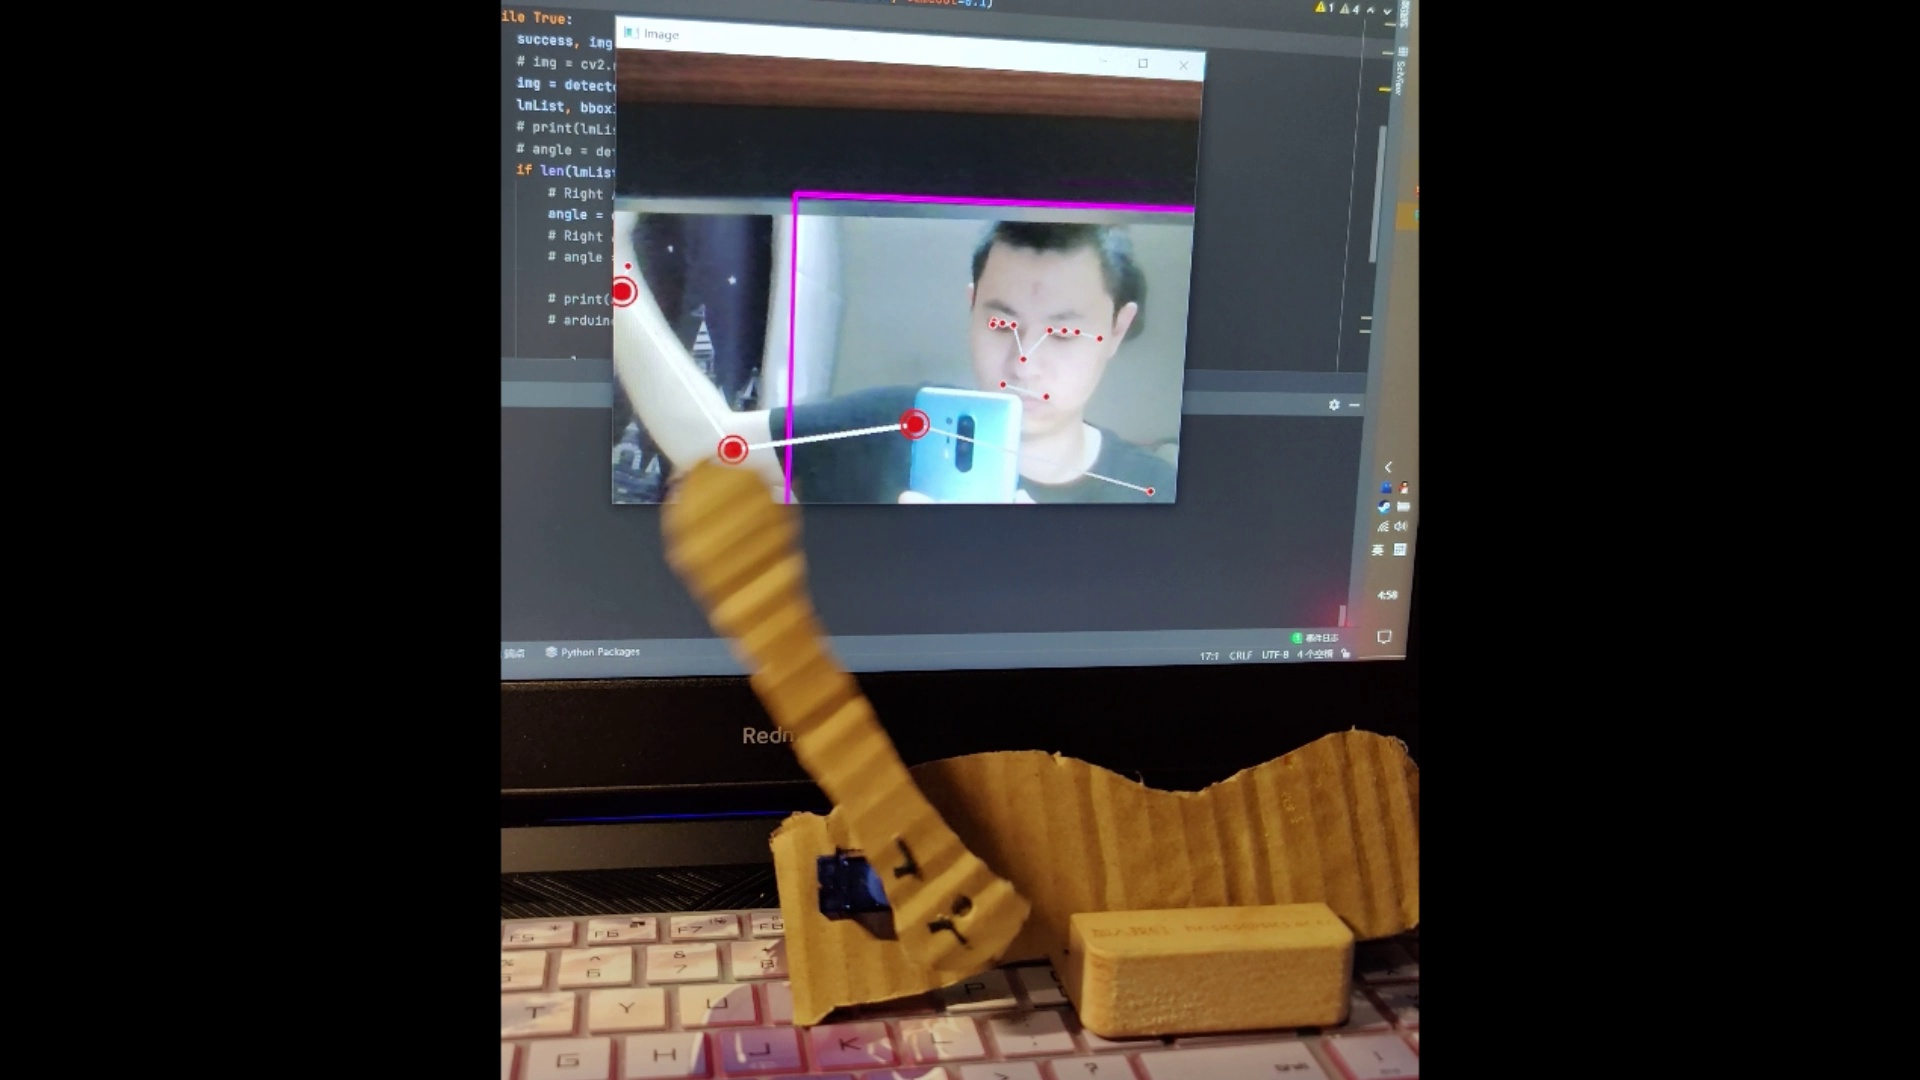
\includegraphics[width=0.31\textwidth]{robot11}}
\subfigure{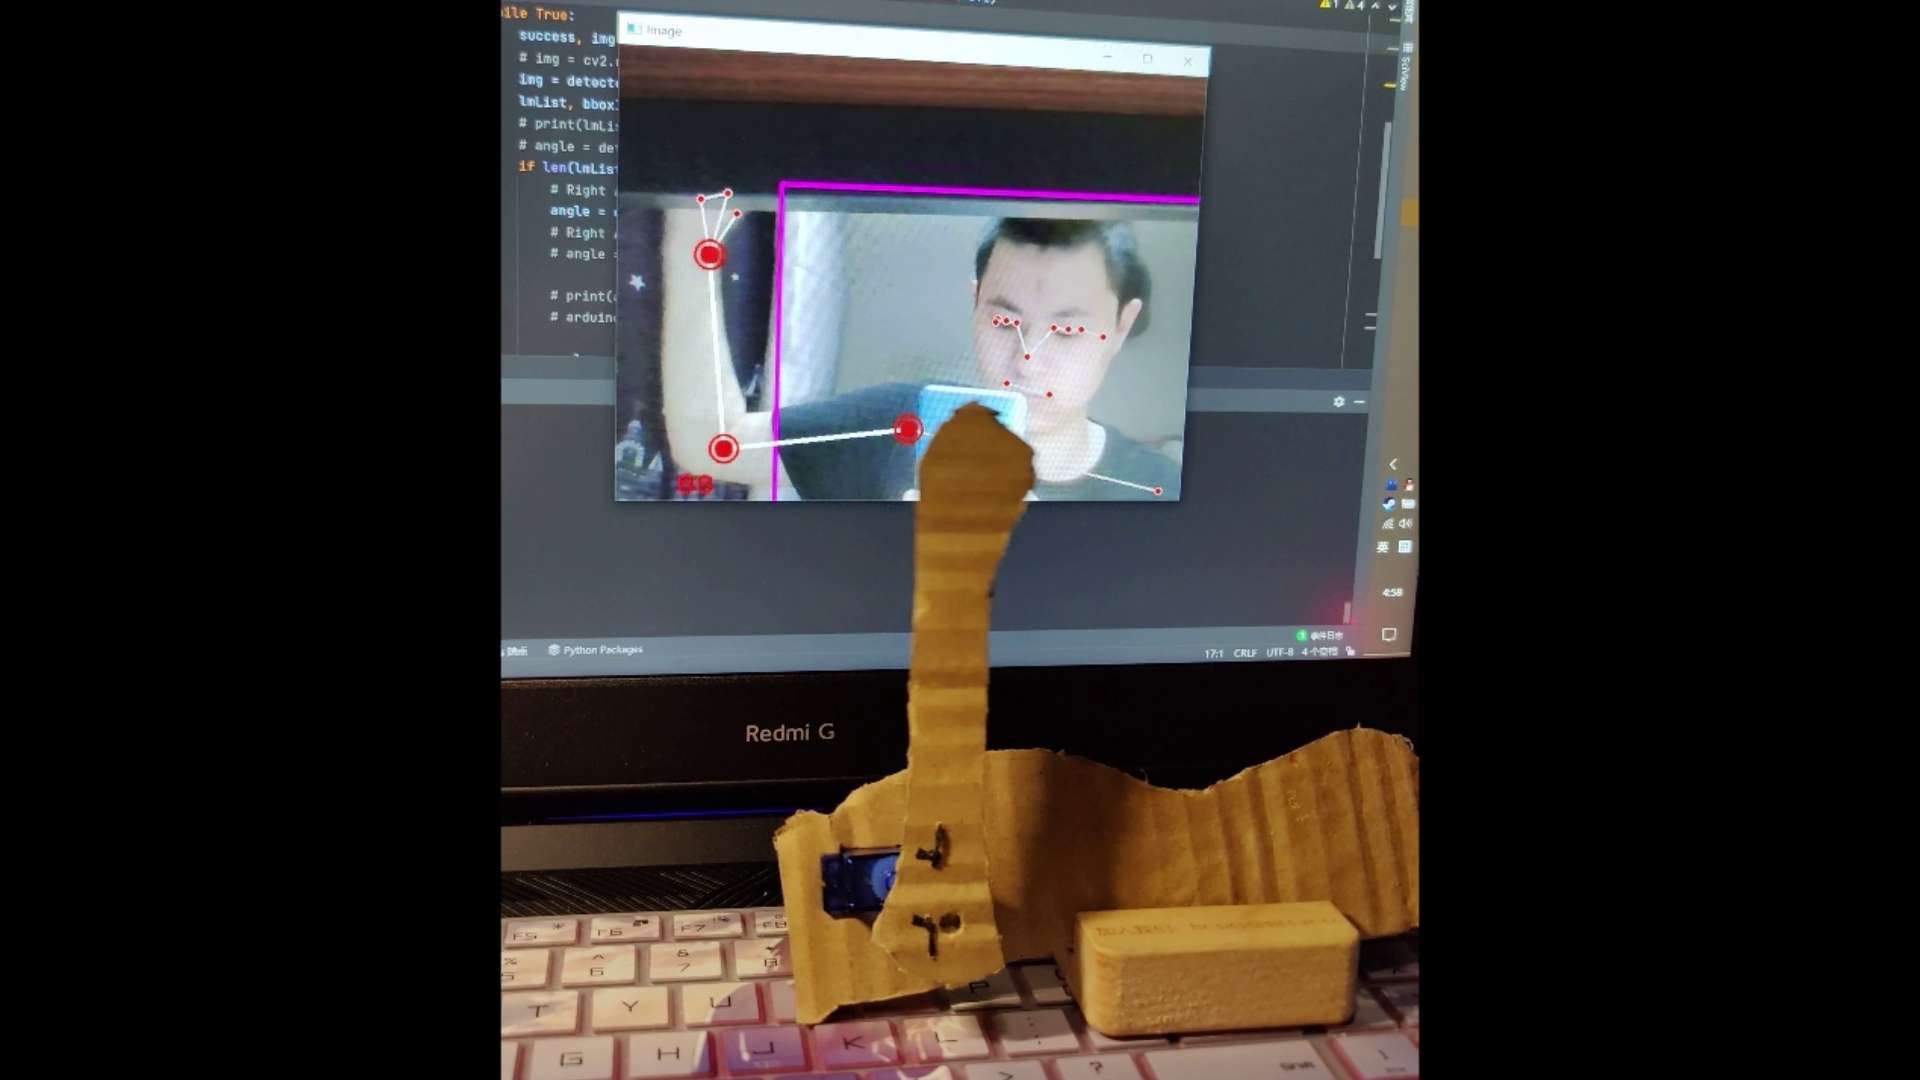
\includegraphics[width=0.31 \textwidth]{robot12}}
\end{minipage}
\vspace{0.2em}
\caption{真实机器人单右肘部姿态模仿截图}
\label{picture:26}
\end{figure}

从时间同步性以及动作准确度的角度来说,当摄像头读取的人体姿态发生变换的同时,机器人也会基本同步完成姿态转变。体现了本模型及时性和轻量化。进一步说明该模型已经达到实用的程度。

\section{本章小结}
本章是实验章节,主要是复现了BlazePose算法,并且将复现的模型与原版模型以及一些主流的模型进行了性能对比,在得到一个可以实用的模型后,本章又将其部署到了电脑端,移动端,虚拟机器人和真实机器人上。最后,得出结论:从机器人模仿的准确度和实时性而言,本项目以达到了预期的效果。


% Local Variables:
% TeX-master: "../main"
% TeX-engine: xetex
% End:
